\chapter{Desenvolvimento Parcial} % TODO: Melhorar isso no futuro e resumir a primeira parte

Esta seção apresenta a etapa inicial de \textit{fine-tuning} do \ac{LLaMA}-3.2, sendo que ela tem um caráter exploratório e visa o desenvolvimento do código base para
os próximos experimentos e também analisar a capacidade de classificação do modelo treinado de diferentes formas.

\section{Tecnologias Utilizadas}

O processamento de dados e \textit{fine-tuning} foram feitos com \textit{scripts} em Python e \textit{Jupyter notebooks}. As dependências do projeto foram gerenciadas
com o gerenciador Poetry e o \textit{framework} de \textit{fine-tuning} utilizado foi o Unsloth. Os treinamentos foram realizados com uma placa NVIDIA H100 de 80 GB que
faz parte de uma plataforma NVIDIA DGX H100.

\section{Conjunto de Dados}

Para os experimentos iniciais, utilizou-se o conjunto de dados \ac{HAM10000} de \textcite{tschandl2018ham10000}, que possui 13354 imagens com informações como a doença
causadora da lesão de pele, a idade do paciente, sexo e localização da lesão. As imagens nesse conjunto de dados são de dermatoscopia.

O conjunto de dados é separado nas seções de treinamento, teste e validação, que possuem 9577, 1285 e 2492 imagens, respectivamente. A \autoref{tab:ham10000_proportion}
apresenta as proporções entre as categorias de lesões de pele. Os dados foram obtidos a partir da plataforma Hugging Face com uma versão do \ac{HAM10000} fornecida por
\textcite{skin_cancer_dataset}.

\begin{table}[ht]
    \caption{\small Proporção entre as diferentes categorias de lesões de pele no \ac{HAM10000}.}
    \centering
    \begin{tabular}{l|c}
        \hline
        Lesão de pele                        & Proporção (\%) \\ \hline
        Nevo melanocítico                    & 66,88          \\
        Melanoma                             & 11,23          \\
        Lesões similares à queratose benigna & 10,94          \\
        \ac{CBC}                             & 5,08           \\
        Queratose actínica                   & 3,29           \\
        Lesões vasculares                    & 1,42           \\
        Dermatofibroma                       & 1,15           \\ \hline
    \end{tabular}
    \label{tab:ham10000_proportion}
    \fonte{\textcite{tschandl2018ham10000}}
\end{table}

\section{Experimentos com \textit{Fine-tuning}}

Os experimentos utilizaram a variante \ac{LLaMA}-3.2-11B-Vision-Instruct, que possui 11 bilhões de parâmetros. Os métodos de \textit{fine-tuning} utilizados foram o
\ac{LoRA} e o \ac{QLoRA}.

\subsection{Dados de treinamento}

O modelo utilizado não suporta ainda a utilização de textos em português para tarefas multimodais, sendo assim, os diálogos estão em inglês. Foi aplicada uma amostragem
estratificada por categoria de lesão de pele sobre os dados de treinamento para que os diálogos tivessem uma representação proporcional de cada lesão. Eles possuem o
seguinte formato:

\begin{dialogue}
    \speak{Usuário} \textit{Classify the skin lesion in the image. \textbf{<imagem>}} \\
    \speak{Modelo} \textit{The skin lesion in the image is \textbf{<lesão de pele>}.}
\end{dialogue}

\subsection{\textit{Fine-tuning} com 450, 900 e 1800 amostras}

% TODO: Ver se é necessário citar os criadores do Adam e AdamW.

A primeira etapa nos experimentos realizar o \textit{fine-tuning} com \ac{QLoRA} com 450 amostras de treinamento e 50 de validação. Os hiperparâmetros\footnote{parâmetros
    de treinamento} utilizados no treinamento estão na \autoref{tab:qlora_500_config}, alguns deles foram omitidos por serem menos relevantes nessa etapa. O \ac{rsLoRA} de
\textcite{kalajdzievski2023rank} foi utilizado para melhorar o desempenho, utilizando um fator de escala \begin{math}\frac{\alpha_{LoRA}}{\sqrt{r}}\end{math} em vez do
\begin{math}\frac{\alpha_{LoRA}}{r}\end{math} do \ac{LoRA} original. Por fim, também foi utilizado o otimizador \ac{Adam} na sua versão paginada de 32 bits. A
\autoref{tab:qlora_500_training} apresenta dados sobre o treinamento e a \autoref{fig:loss_qlora_500} apresenta o \textit{loss} de treinamento e validação ao longo dos
passos.

\begin{table}[ht]
    \caption{\small Hiperparâmetros para o \ac{QLoRA} com 450, 900 e 1800 amostras. A primeira seção se refere às configurações específicas de \ac{PEFT}, enquanto a
        segunda se refere ao treinamento em geral.}
    \centering
    \begin{tabular}{l|c}
        \hline
        Hiperparâmetro                             & Valor                                  \\ \hline
        Camadas e módulos treinados                & Visão, linguagem, atenção e \ac{MLP}   \\
        Rank                                       & 32                                     \\
        Alfa (\begin{math}\alpha_{LoRA}\end{math}) & 32                                     \\
        Dropout                                    & 0,1                                    \\
        \ac{rsLoRA}                                & Sim                                    \\ \hline
        Taxa de aprendizado                        & \begin{math}2 \times 10^{-4}\end{math} \\
        Razão de aquecimento                       & 0,03                                   \\
        Tipo de escalonador da taxa de aprendizado & Cosseno com reinícios                  \\
        Decaimento de peso                         & 0,01                                   \\
        Épocas                                     & 5                                      \\
        Passos a cada validação                    & 50                                     \\
        Otimizador                                 & \ac{Adam} paginado de 32 bits          \\
        Tipo numérico                              & \ac{BF16}                              \\ \hline
    \end{tabular}
    \label{tab:qlora_500_config}
    \fonte{Autoria própria}
\end{table}

\begin{table}[ht]
    \caption{\small Dados sobre o treinamento com \ac{QLoRA} com 450 amostras.}
    \centering
    \begin{tabular}{l|c}
        \hline
                                    & Valor     \\ \hline
        Parâmetros treináveis       & 134348800 \\
        Tempo de treinamento (min)  & 16,17     \\
        Passos                      & 110       \\
        Memória máxima alocada (GB) & 18.69     \\ \hline
    \end{tabular}
    \label{tab:qlora_500_training}
    \fonte{Autoria própria}
\end{table}

\begin{figure}[ht]
    \centering
    \caption{\small \textit{Loss} de treinamento e validação para o \ac{QLoRA} com 450 amostras.}
    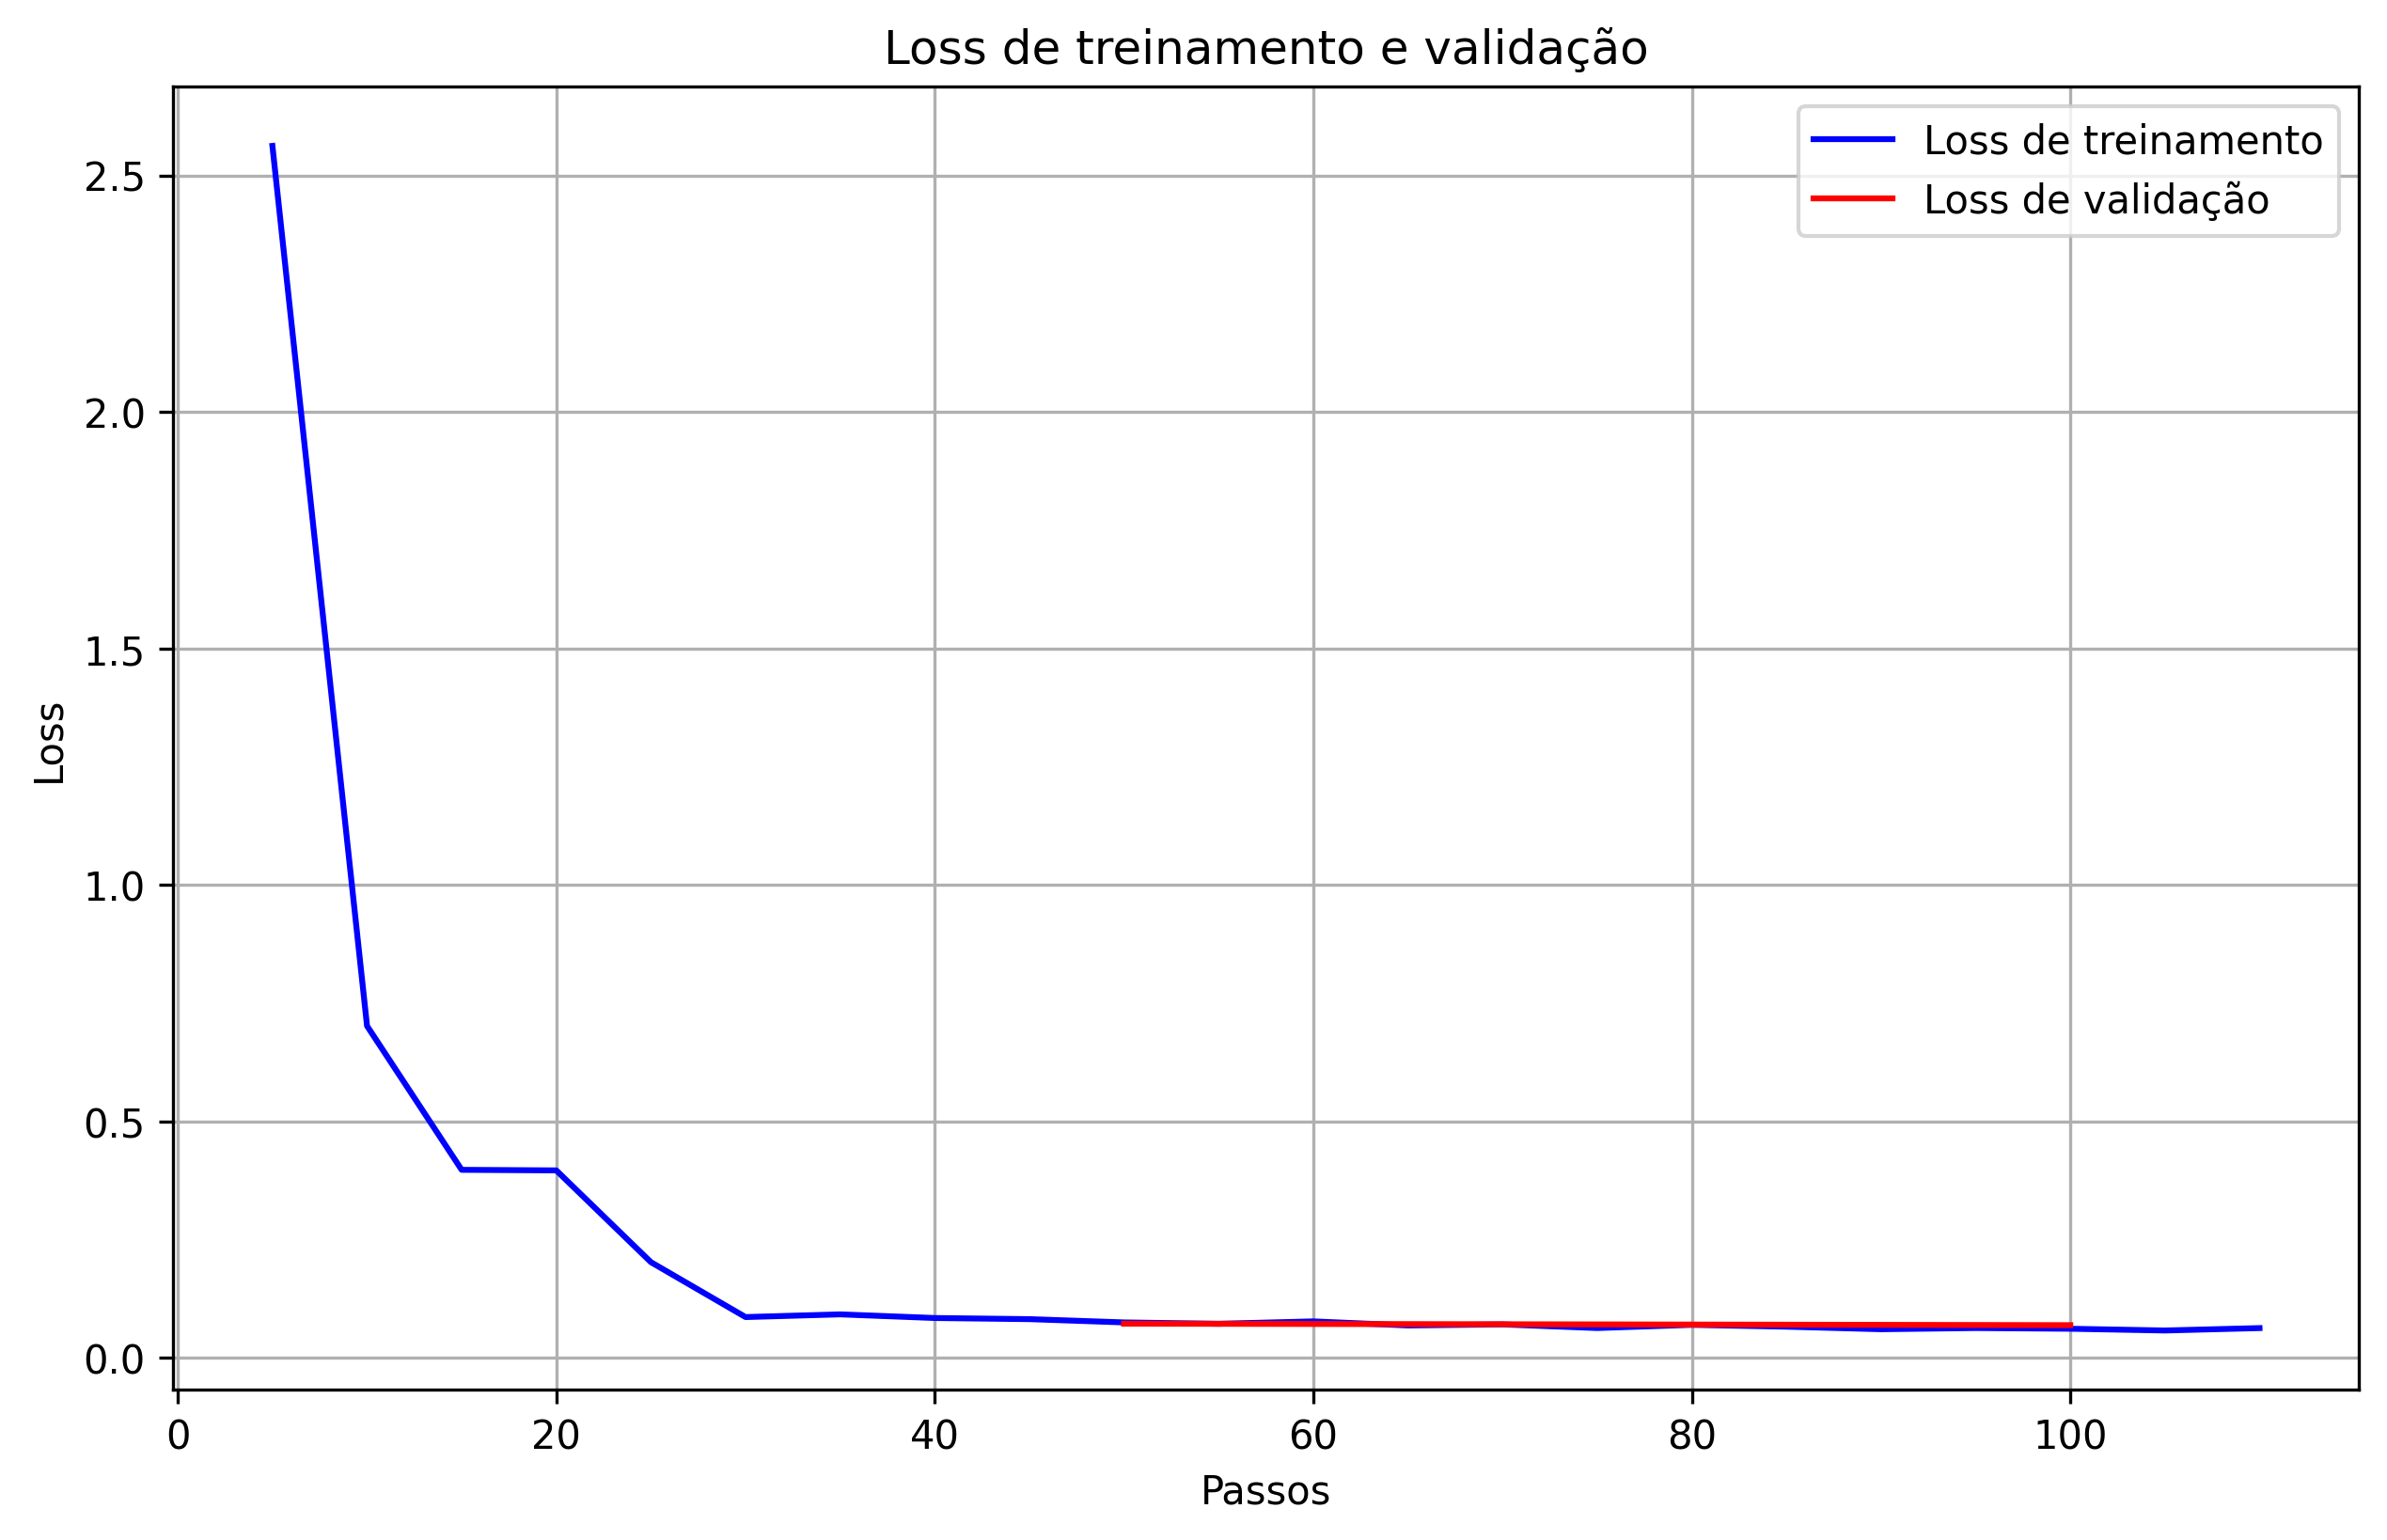
\includegraphics[width=0.8\columnwidth,keepaspectratio]{images/loss_qlora_500.png}
    \label{fig:loss_qlora_500}
    \fonte{Autoria própria.}
\end{figure}

Em seguida, foi realizado o \textit{fine-tuning} com \ac{LoRA}, ou seja, sem quantização, com 450 amostras. Os hiperparâmetros utilizados são similares, porém, o
\textit{rank} foi reduzido para 16, assim como o \begin{math}\alpha_{LoRA}\end{math}. O \ac{rsLoRA} não foi utilizado e a taxa de aprendizado foi reduzida a
\begin{math}1 \times 10^{-4}\end{math}. Por fim o otimizador \ac{AdamW} foi utilizado. A \autoref{tab:lora_500_training} apresenta os dados de treinamento e a
\autoref{fig:loss_lora_500} apresenta o \textit{loss}. O treinamento foi aplicado somente sobre 64174400 parâmetros, uma quantidade menor do que a usada no
\ac{QLoRA} por conta do \textit{rank} reduzido.

\begin{table}[ht]
    \caption{\small Dados sobre o treinamento com \ac{LoRA} com 450 amostras.}
    \centering
    \begin{tabular}{l|c}
        \hline
                                    & Valor    \\ \hline
        Parâmetros treináveis       & 64174400 \\
        Tempo de treinamento (min)  & 26,42    \\
        Passos                      & 140      \\
        Memória máxima alocada (GB) & 40,35    \\ \hline
    \end{tabular}
    \label{tab:lora_500_training}
    \fonte{Autoria própria}
\end{table}

\clearpage

\begin{figure}[ht]
    \centering
    \caption{\small \textit{Loss} de treinamento e validação para o \ac{LoRA} com 450 amostras.}
    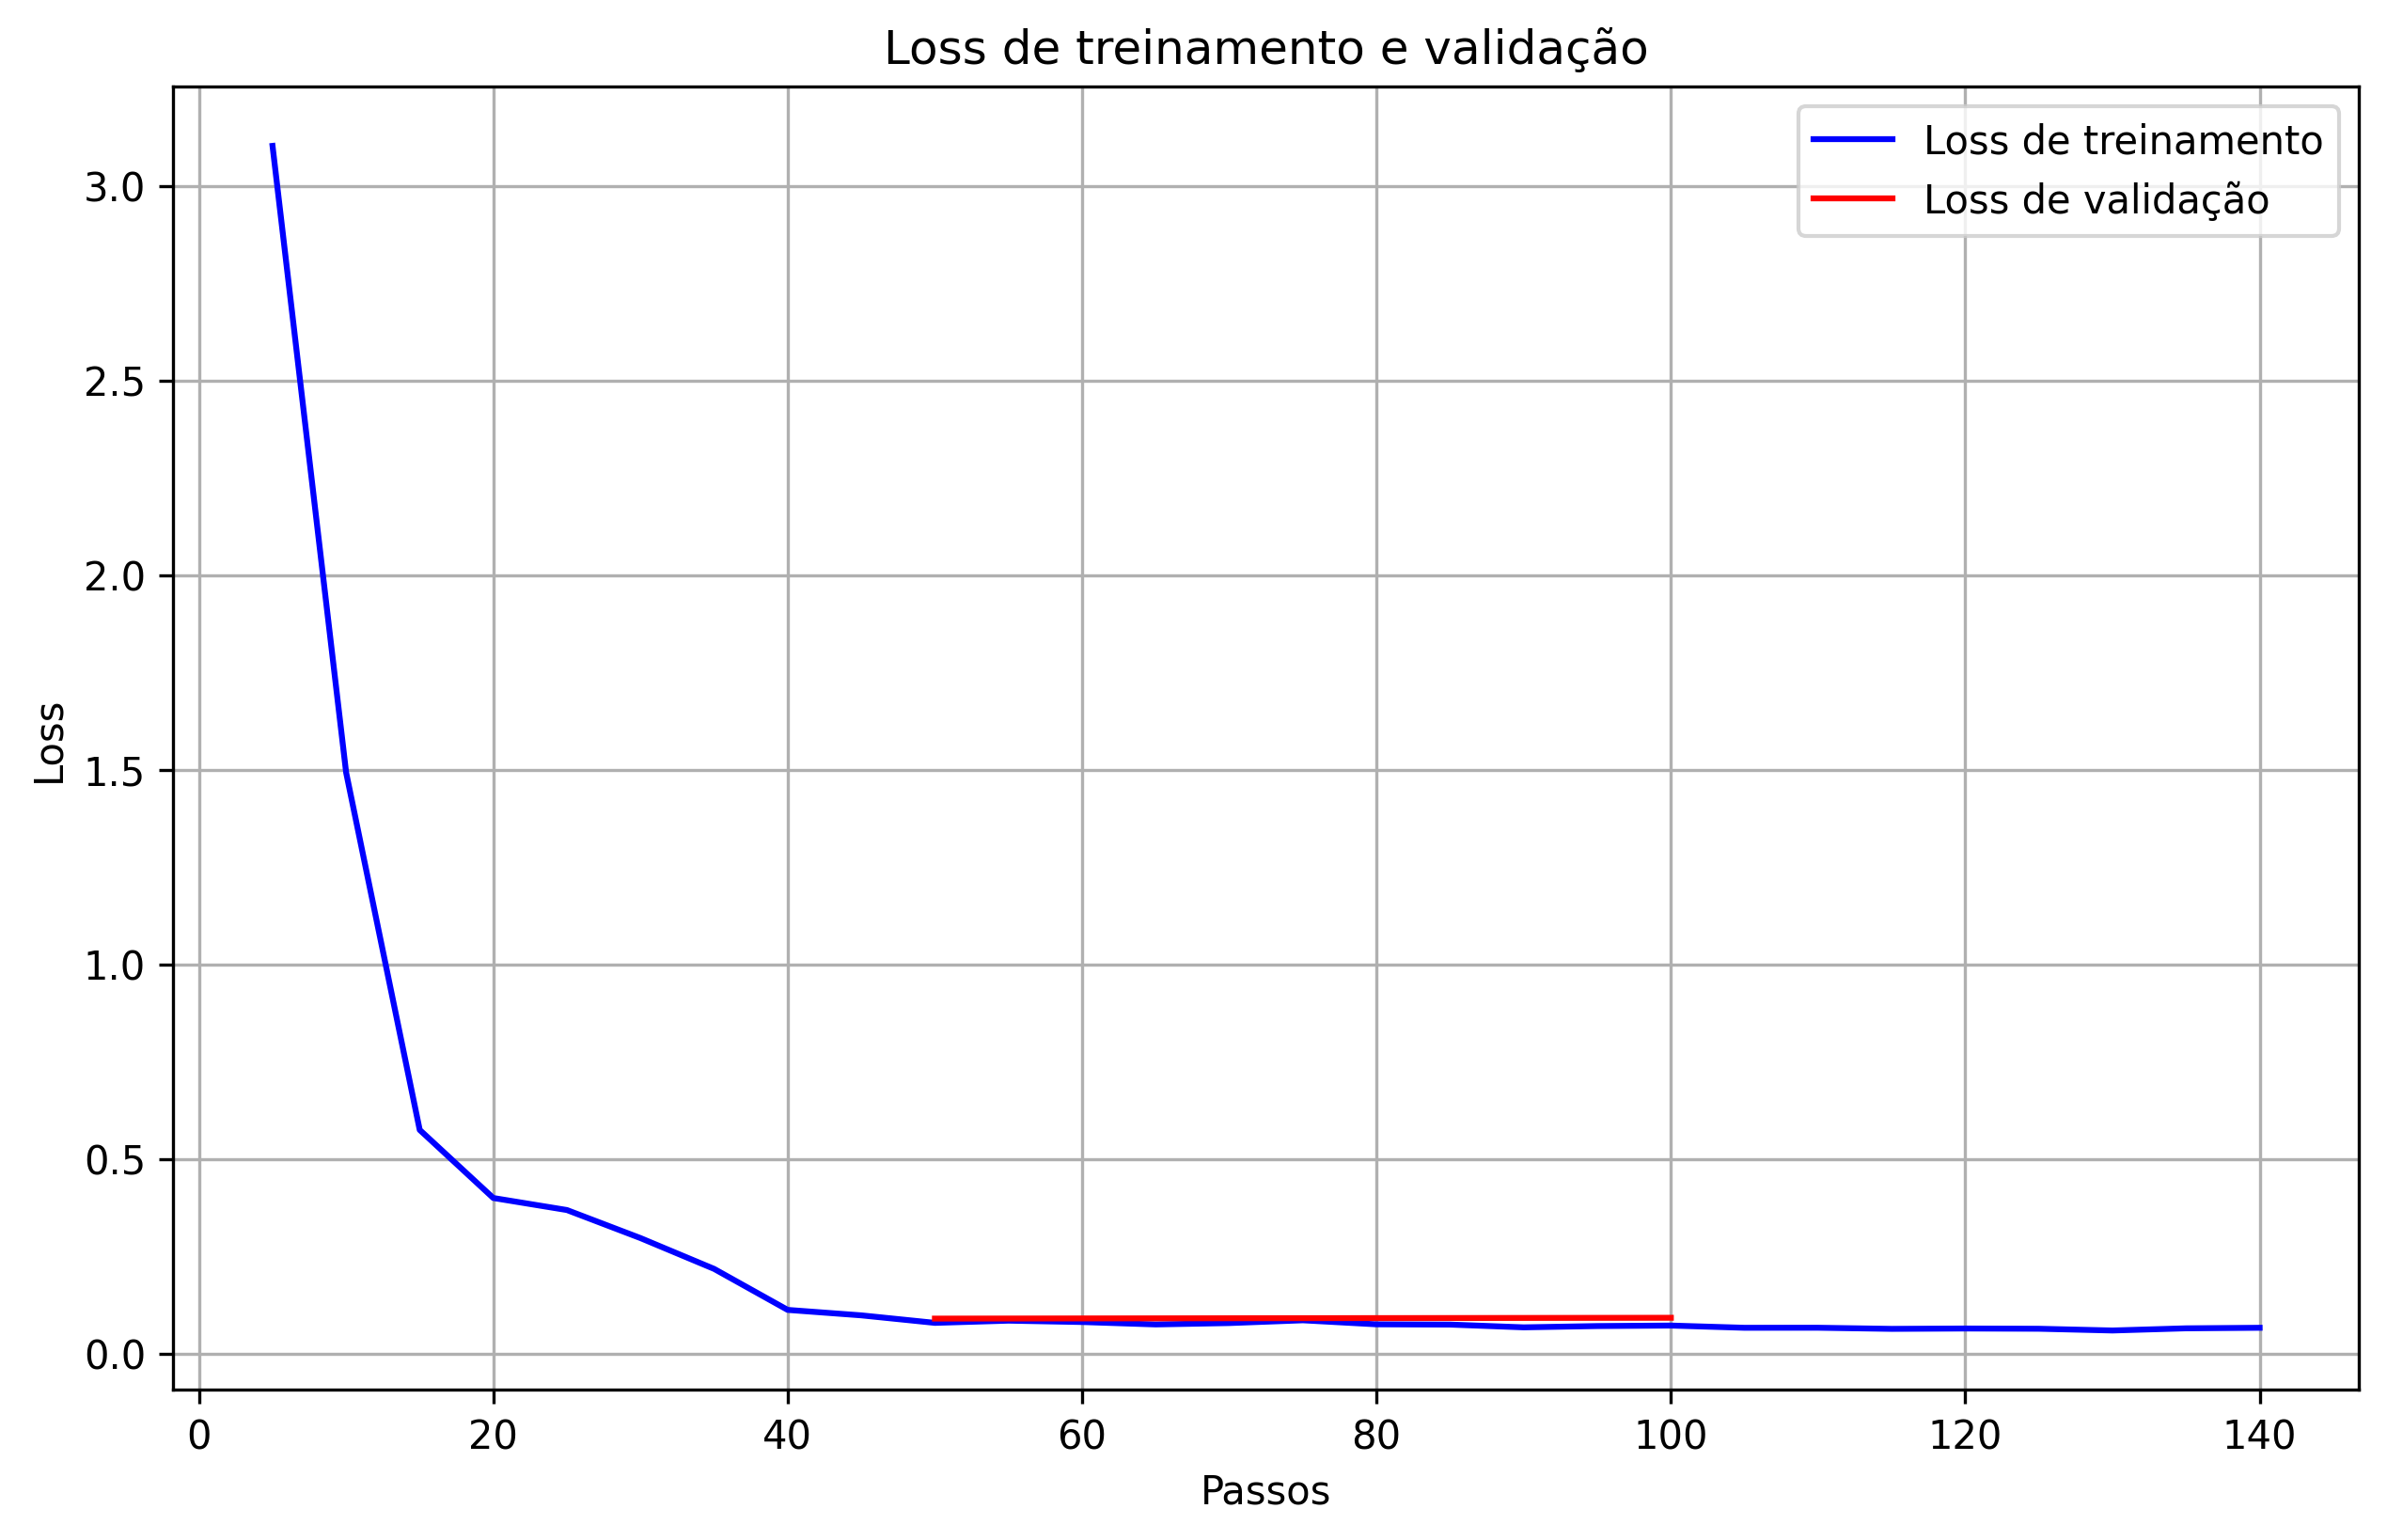
\includegraphics[width=0.725\columnwidth,keepaspectratio]{images/loss_lora_500.png}
    \label{fig:loss_lora_500}
    \fonte{Autoria própria.}
\end{figure}

O \textit{fine-tuning} com 900 amostras foi feito sem a alteração nos hiperparâmetros do \ac{QLoRA} e \ac{LoRA}. As informações sobre o treinamento podem ser conferidas
na \autoref{tab:qlora_1000_training} e \autoref{tab:lora_1000_training}, enquanto o \textit{loss} pode ser conferido na \autoref{fig:loss_qlora_1000} e
\autoref{fig:loss_lora_1000}.

\begin{table}[ht]
    \caption{\small Dados sobre o treinamento com \ac{QLoRA} com 900 amostras.}
    \centering
    \begin{tabular}{l|c}
        \hline
                                    & Valor     \\ \hline
        Parâmetros treináveis       & 134348800 \\
        Tempo de treinamento (min)  & 32,08     \\
        Passos                      & 225       \\
        Memória máxima alocada (GB) & 18,695    \\ \hline
    \end{tabular}
    \label{tab:qlora_1000_training}
    \fonte{Autoria própria}
\end{table}

\begin{table}[ht]
    \caption{\small Dados sobre o treinamento com \ac{LoRA} com 900 amostras.}
    \centering
    \begin{tabular}{l|c}
        \hline
                                    & Valor    \\ \hline
        Parâmetros treináveis       & 67174400 \\
        Tempo de treinamento (min)  & 41,76    \\
        Passos                      & 280      \\
        Memória máxima alocada (GB) & 31,965   \\ \hline
    \end{tabular}
    \label{tab:lora_1000_training}
    \fonte{Autoria própria}
\end{table}

\clearpage

\begin{figure}[ht]
    \centering
    \caption{\small \textit{Loss} de treinamento e validação para o \ac{QLoRA} com 900 amostras.}
    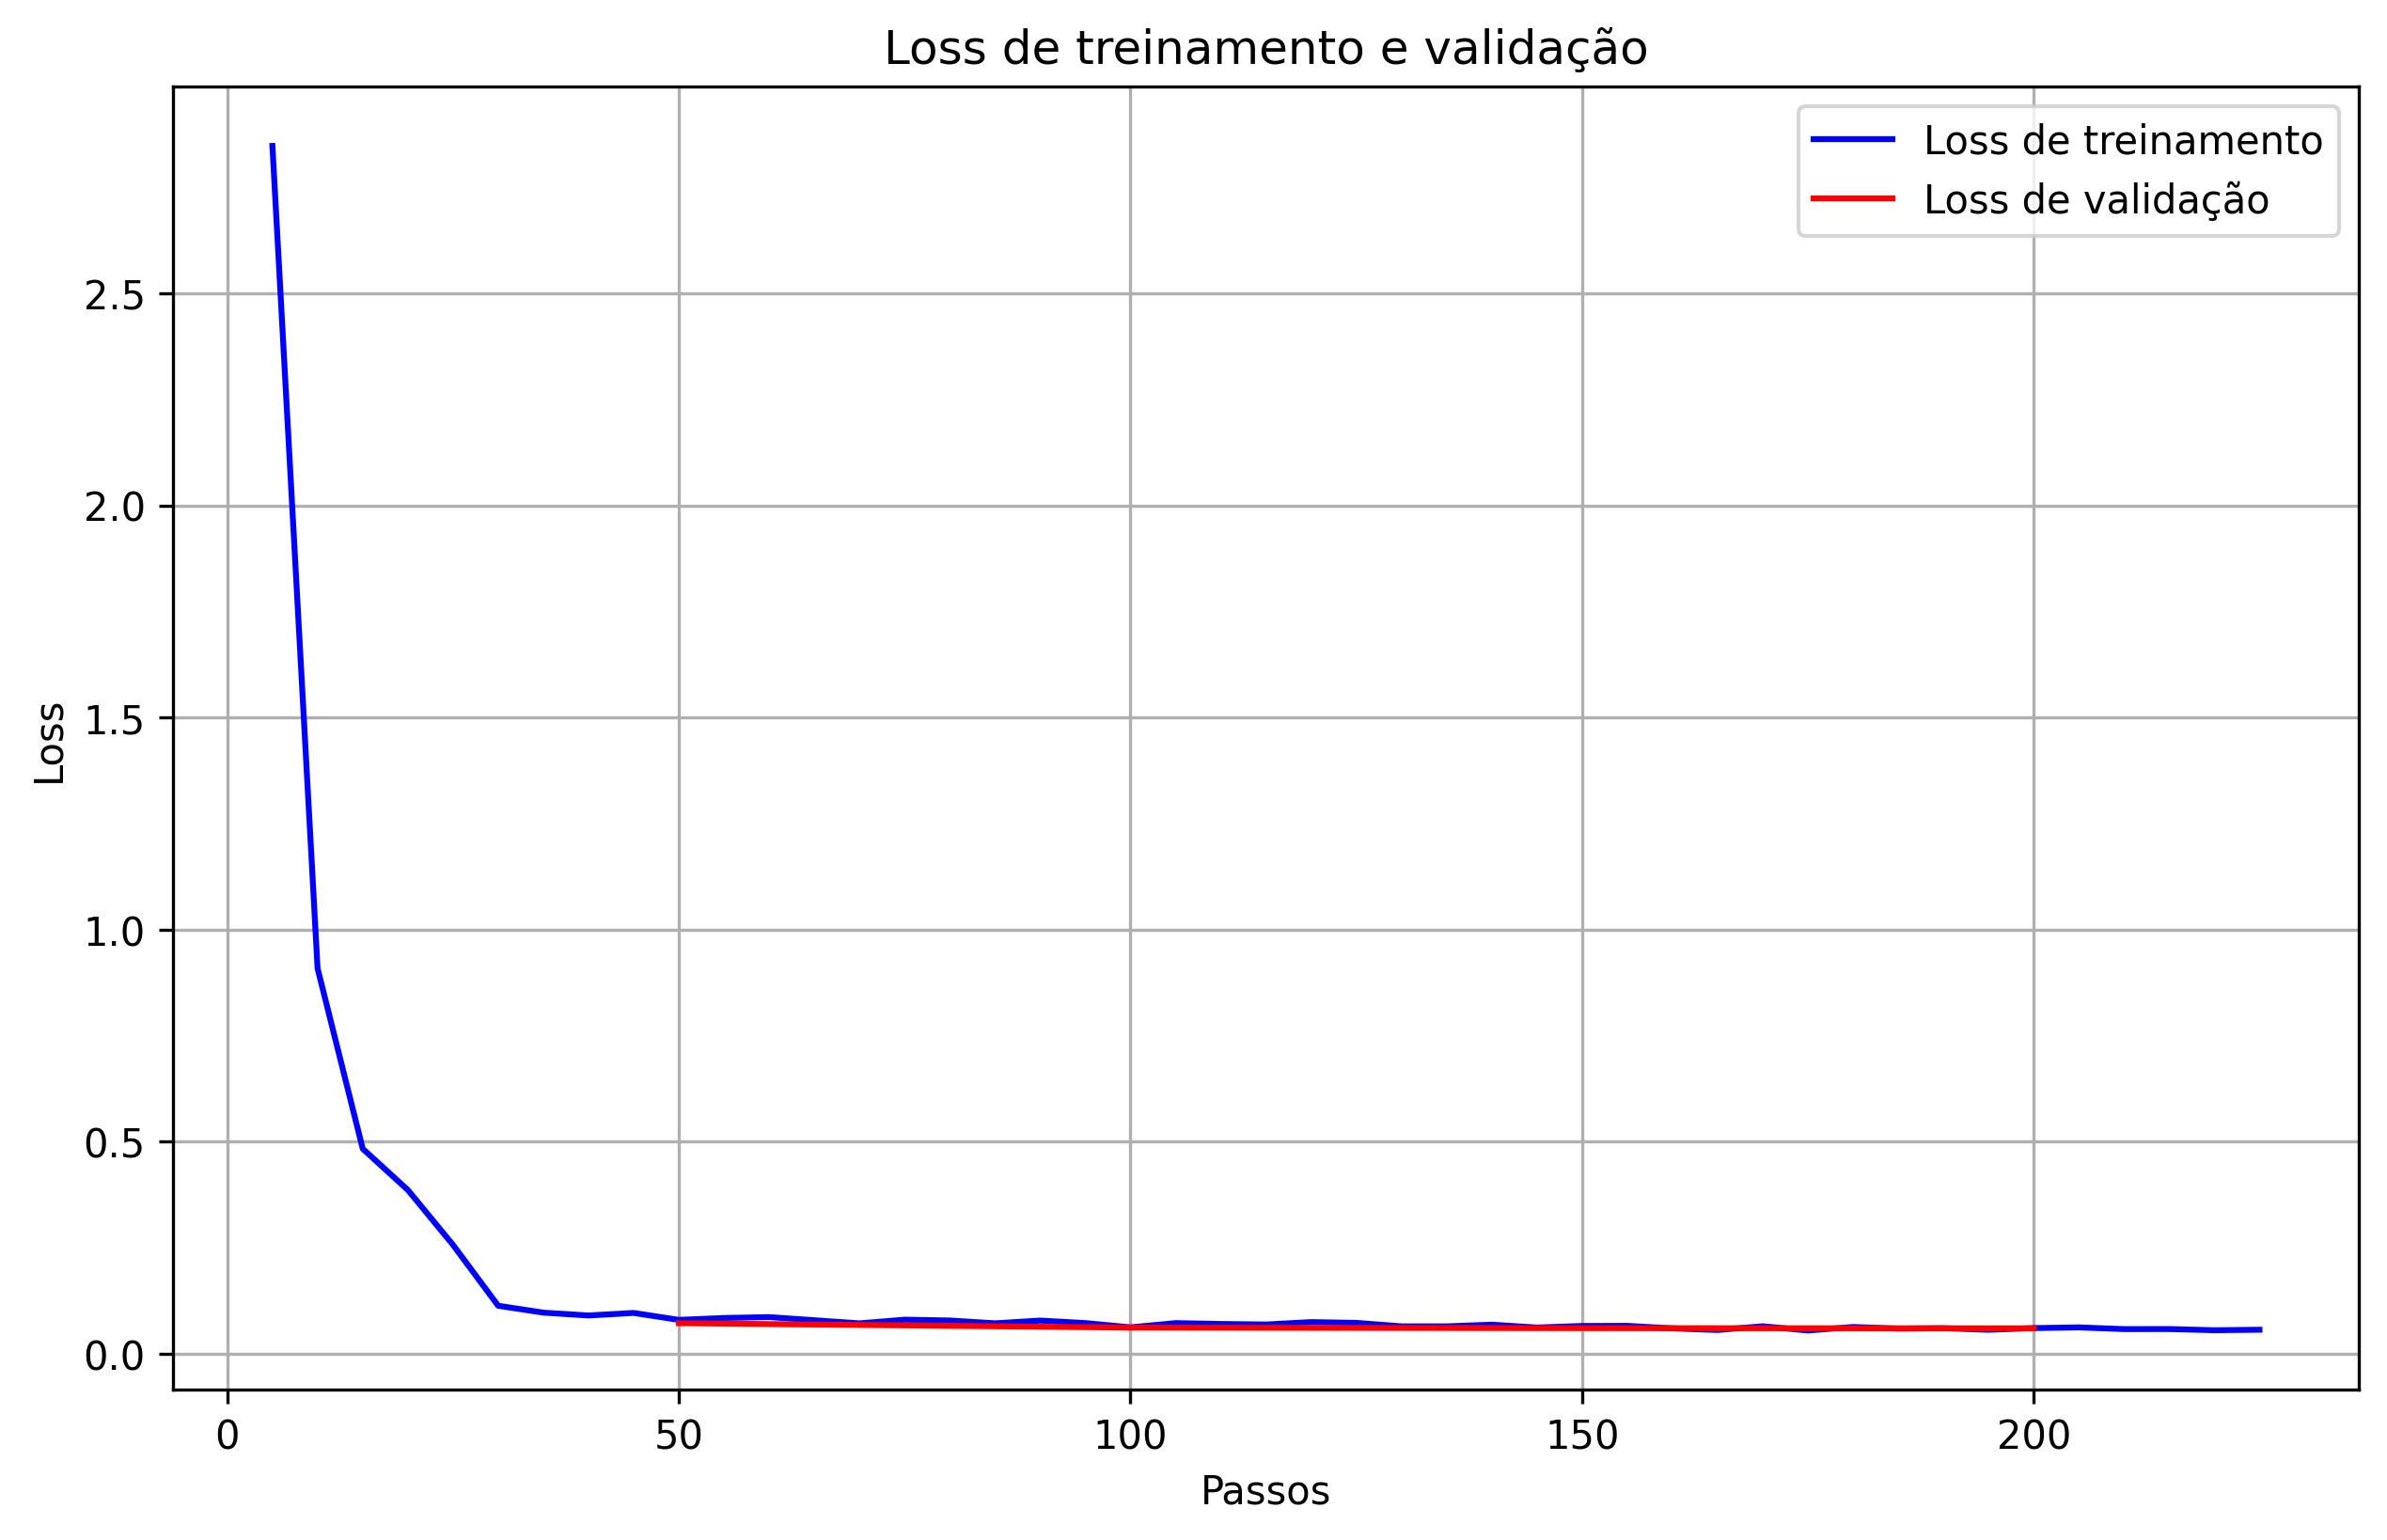
\includegraphics[width=0.725\columnwidth,keepaspectratio]{images/loss_qlora_1000.png}
    \label{fig:loss_qlora_1000}
    \fonte{Autoria própria.}
\end{figure}

\begin{figure}[ht]
    \centering
    \caption{\small \textit{Loss} de treinamento e validação para o \ac{LoRA} com 900 amostras.}
    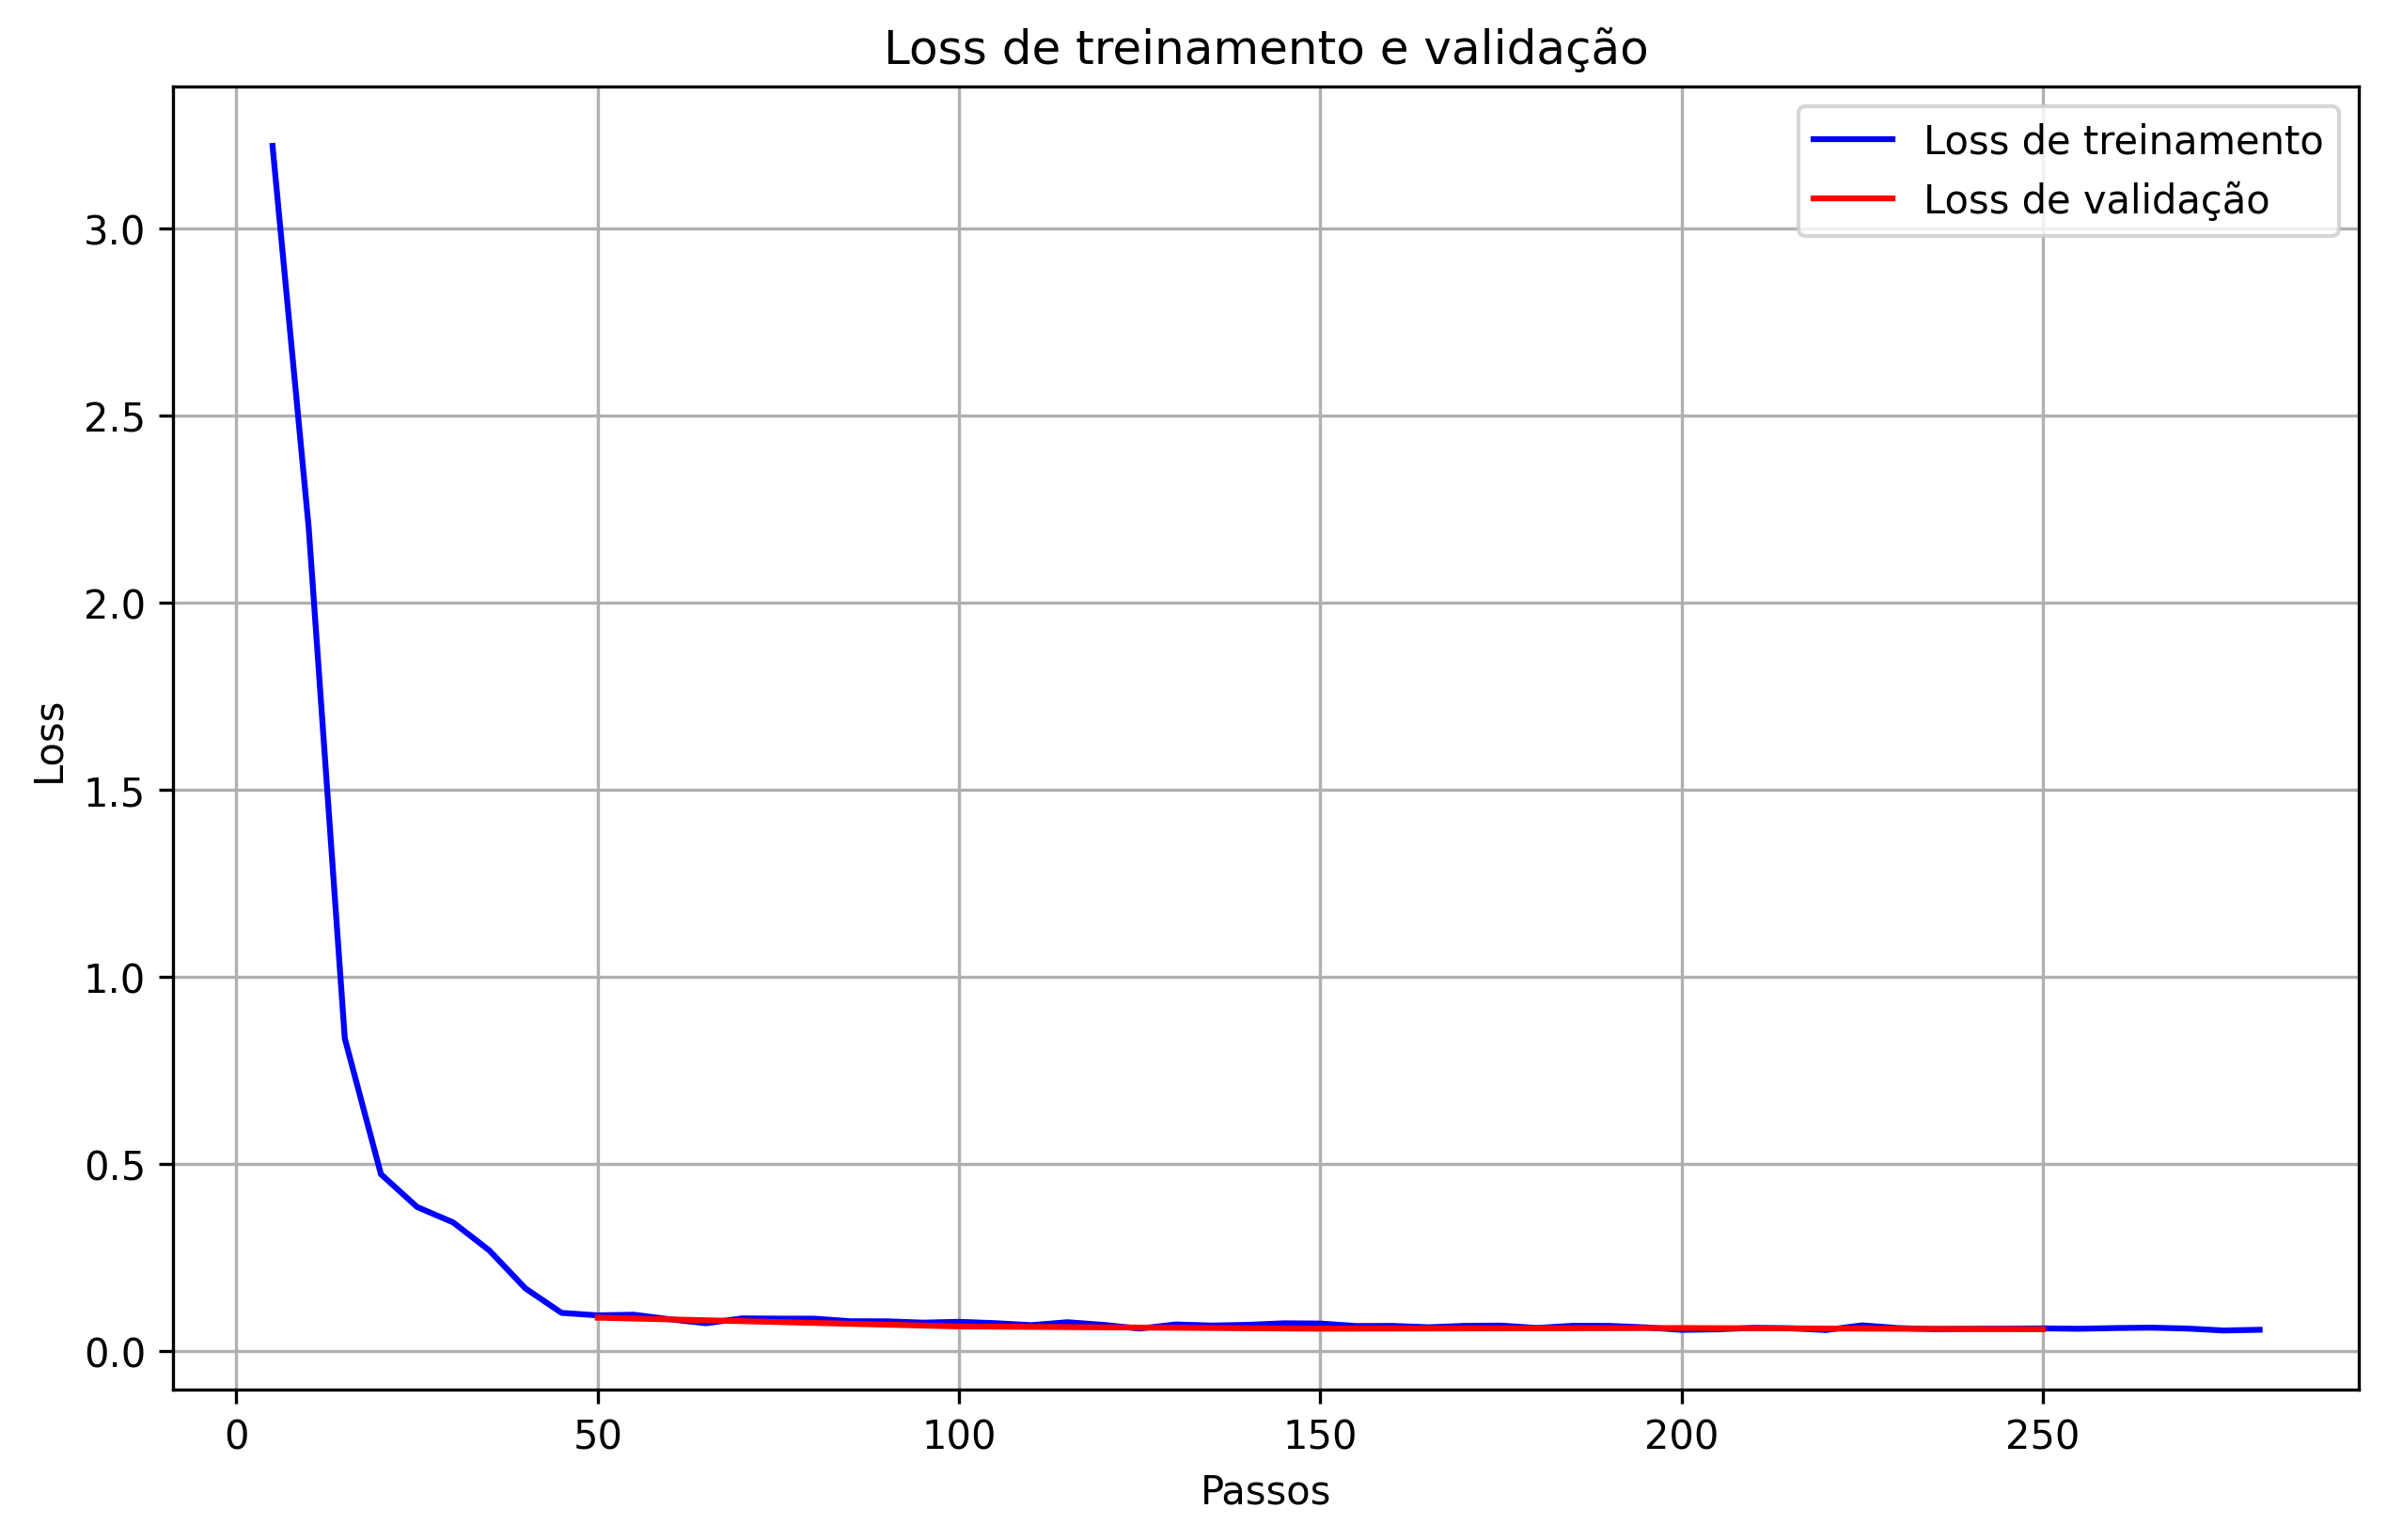
\includegraphics[width=0.725\columnwidth,keepaspectratio]{images/loss_lora_1000.png}
    \label{fig:loss_lora_1000}
    \fonte{Autoria própria.}
\end{figure}

Por último, foi feito um \textit{fine-tuning} com \ac{QLoRA} com 1800 amostras com os mesmos hiperparâmetros utilizados anteriormente. As informações sobre o treinamento
podem ser vistas na \autoref{tab:qlora_2000_training} e na \autoref{fig:loss_qlora_2000}.

\clearpage

\begin{table}[ht]
    \caption{\small Dados sobre o treinamento com \ac{QLoRA} com 1800 amostras.}
    \centering
    \begin{tabular}{l|c}
        \hline
                                    & Valor     \\ \hline
        Parâmetros treináveis       & 134348800 \\
        Tempo de treinamento (min)  & 90,77     \\
        Passos                      & 450       \\
        Memória máxima alocada (GB) & 18,744    \\ \hline
    \end{tabular}
    \label{tab:qlora_2000_training}
    \fonte{Autoria própria}
\end{table}

\begin{figure}[ht]
    \centering
    \caption{\small \textit{Loss} de treinamento e validação para o \ac{QLoRA} com 1800 amostras.}
    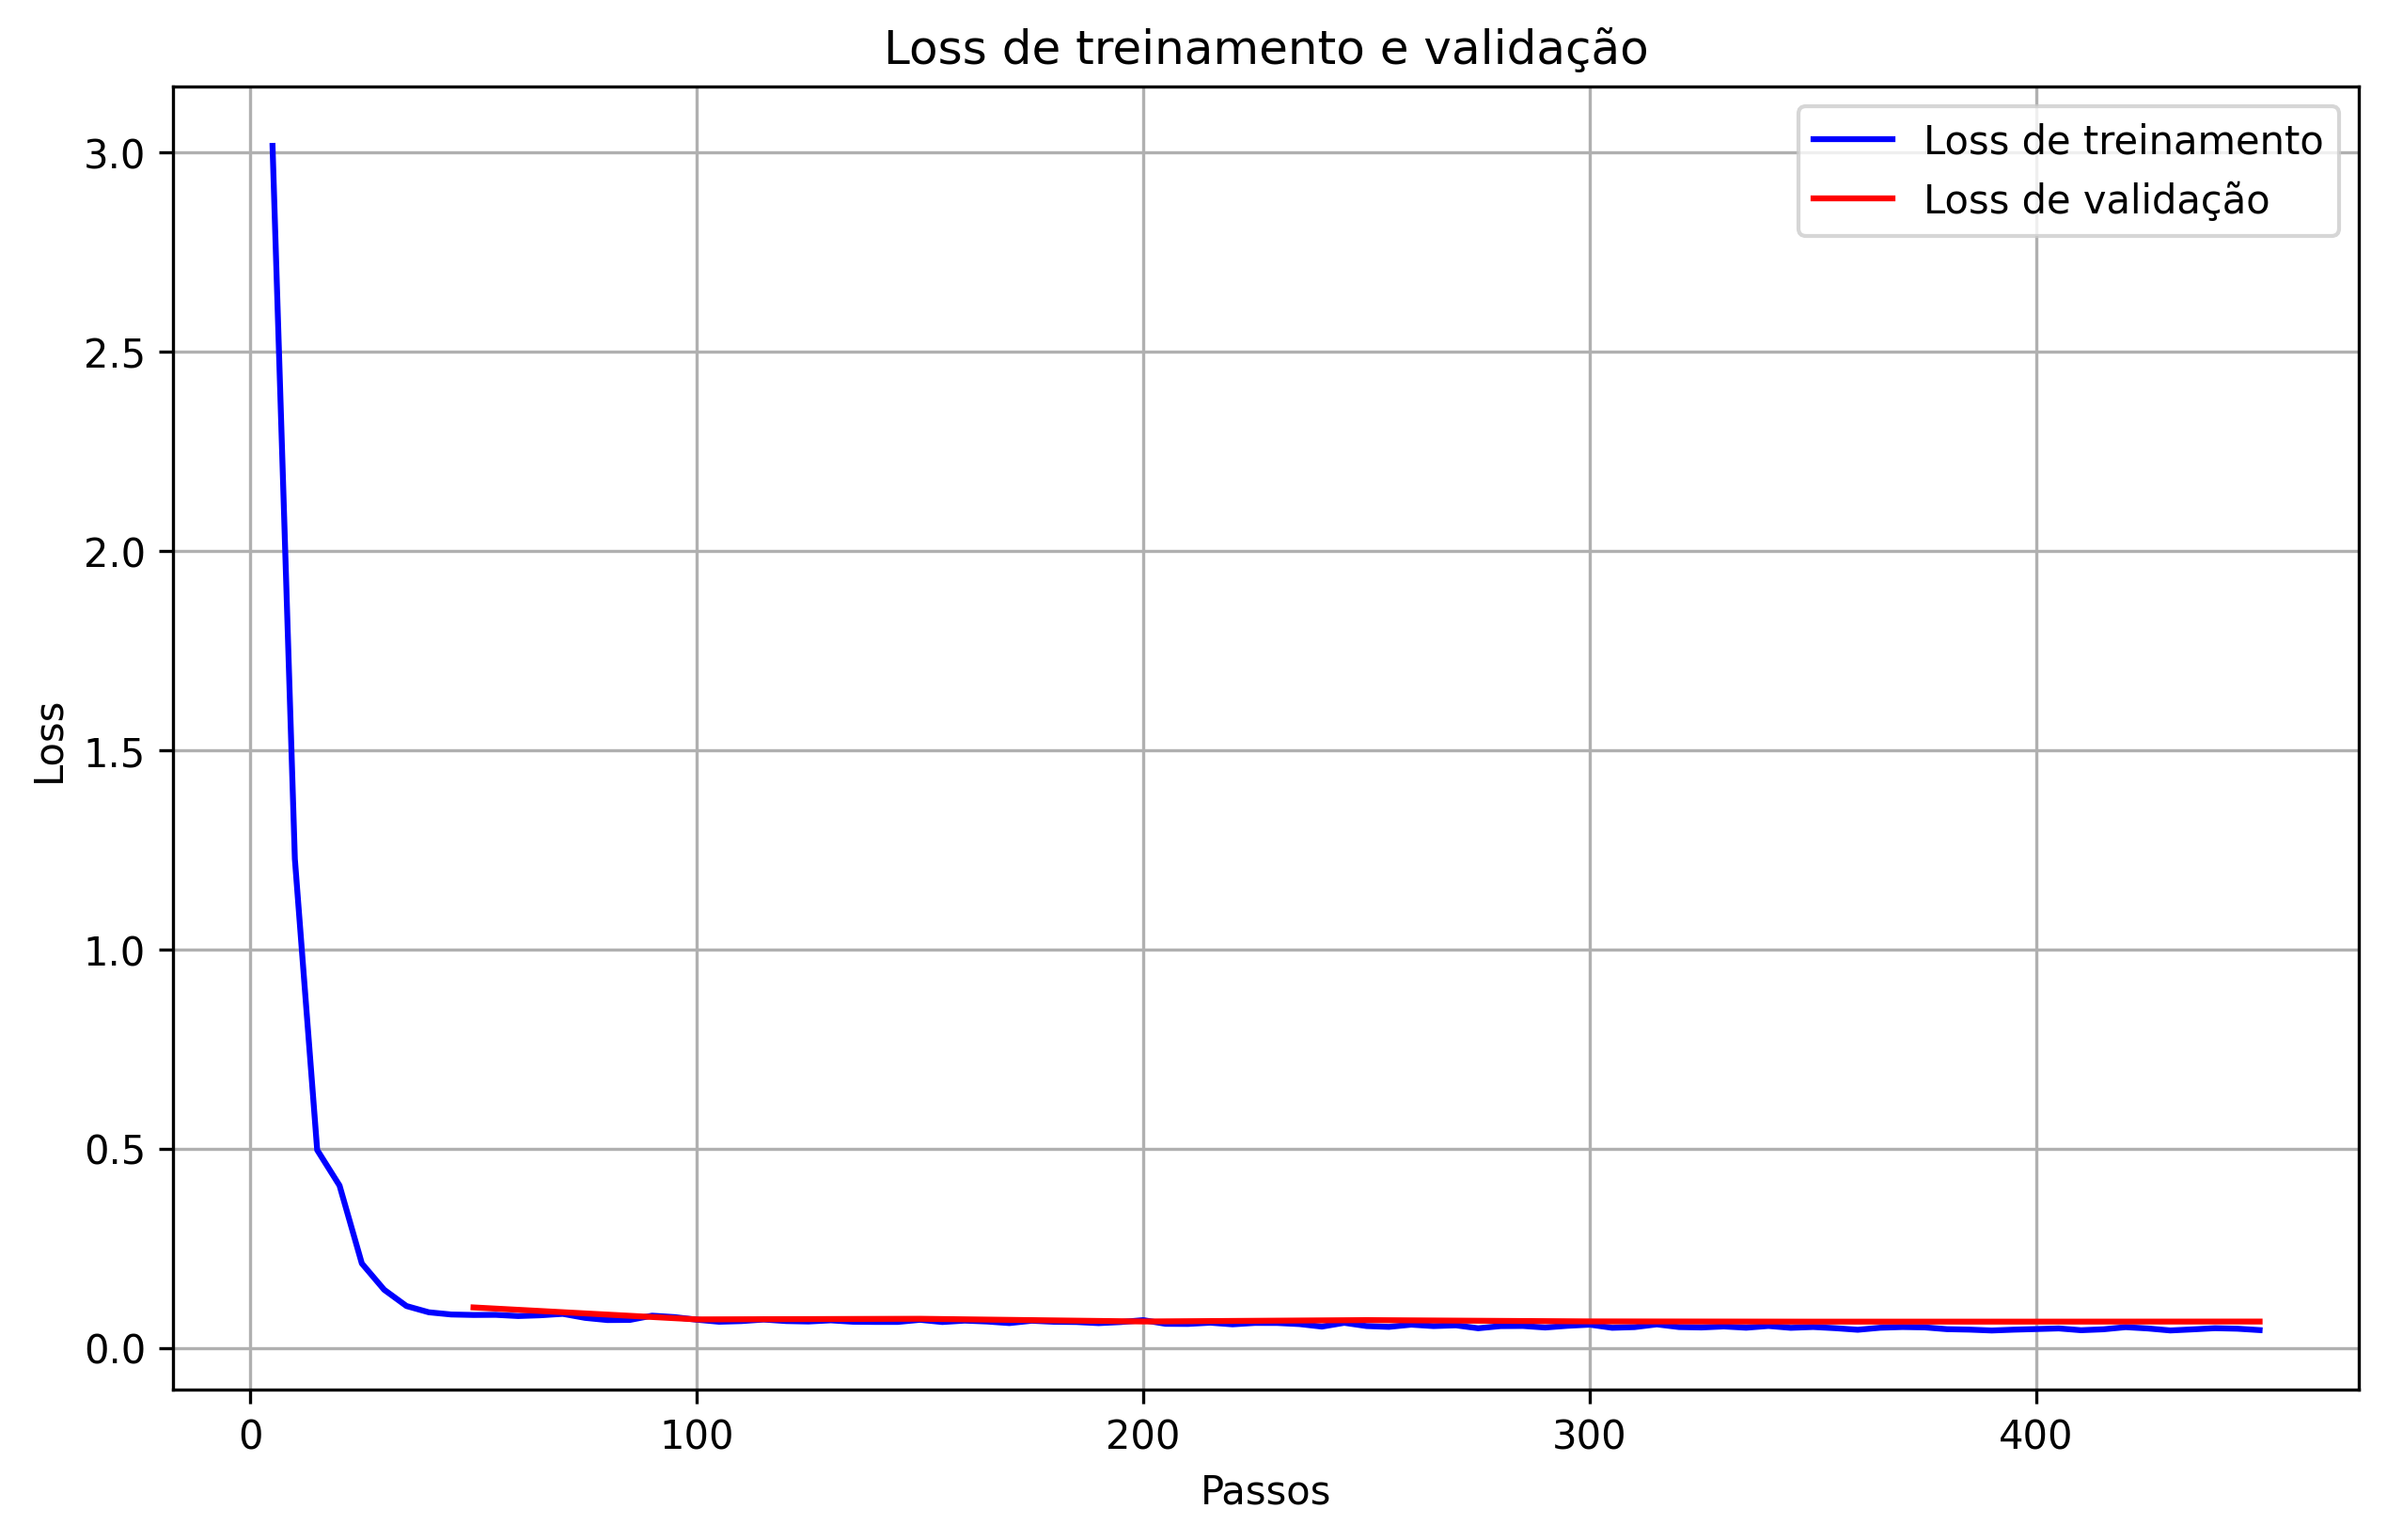
\includegraphics[width=0.725\columnwidth,keepaspectratio]{images/loss_qlora_2000.png}
    \label{fig:loss_qlora_2000}
    \fonte{Autoria própria.}
\end{figure}

\subsection{\textit{Fine-tuning} com 5000 e 9500 amostras}

Para avaliar o impacto de diferentes hiperparâmetros, foram feitos \textit{fine-tunings} modificados com 5000 e 9500 amostras. As configurações na
\autoref{tab:qlora_5000_config} se referem tanto ao \ac{QLoRA} quanto ao \ac{LoRA}. Foi utilizado somente o \ac{QLoRA} no treinamento com 9500 amostras. Os dados dos
treinamentos podem ser conferidos na \autoref{tab:qlora_5000_training}, \autoref{tab:lora_5000_training} e \autoref{tab:qlora_9500_training}, enquanto o \textit{loss}
pode ser conferido na \autoref{fig:loss_qlora_5000}, \autoref{fig:loss_lora_5000} e \autoref{fig:loss_qlora_9500}.

\clearpage

\begin{table}[ht]
    \caption{\small Hiperparâmetros para o \textit{fine-tuning} com 5000 e 9500 amostras. A primeira seção se refere às configurações específicas de \ac{PEFT}, enquanto
        a segunda se refere ao treinamento em geral.}
    \centering
    \begin{tabular}{l|c}
        \hline
        Hiperparâmetro                             & Valor                                  \\ \hline
        Camadas e módulos treinados                & Visão, linguagem, atenção e \ac{MLP}   \\
        Rank                                       & 64                                     \\
        Alfa (\begin{math}\alpha_{LoRA}\end{math}) & 64                                     \\
        Dropout                                    & 0,05                                   \\
        \ac{rsLoRA}                                & Sim                                    \\ \hline
        Taxa de aprendizado                        & \begin{math}1 \times 10^{-4}\end{math} \\
        Razão de aquecimento                       & 0                                      \\
        Tipo de escalonador da taxa de aprendizado & Constante                              \\
        Decaimento de peso                         & 0,01                                   \\
        Épocas                                     & 3                                      \\
        Passos a cada validação                    & A cada 5\% dos passos                  \\
        Otimizador                                 & \ac{Adam} paginado de 32 bits          \\
        Tipo numérico                              & \ac{BF16}                              \\ \hline
    \end{tabular}
    \label{tab:qlora_5000_config}
    \fonte{Autoria própria}
\end{table}

\begin{table}[ht]
    \caption{\small Dados sobre o treinamento com \ac{QLoRA} com 5000 amostras.}
    \centering
    \begin{tabular}{l|c}
        \hline
                                    & Valor     \\ \hline
        Parâmetros treináveis       & 268697600 \\
        Tempo de treinamento (min)  & 96,63     \\
        Passos                      & 1875      \\
        Memória máxima alocada (GB) & 18,967    \\ \hline
    \end{tabular}
    \label{tab:qlora_5000_training}
    \fonte{Autoria própria}
\end{table}

\begin{table}[ht]
    \caption{\small Dados sobre o treinamento com \ac{LoRA} com 5000 amostras.}
    \centering
    \begin{tabular}{l|c}
        \hline
                                    & Valor     \\ \hline
        Parâmetros treináveis       & 268697600 \\
        Tempo de treinamento (min)  & 100,33    \\
        Passos                      & 1875      \\
        Memória máxima alocada (GB) & 31,48     \\ \hline
    \end{tabular}
    \label{tab:lora_5000_training}
    \fonte{Autoria própria}
\end{table}

\clearpage

\begin{table}[ht]
    \caption{\small Dados sobre o treinamento com \ac{QLoRA} com 9500 amostras.}
    \centering
    \begin{tabular}{l|c}
        \hline
                                    & Valor     \\ \hline
        Parâmetros treináveis       & 268697600 \\
        Tempo de treinamento (min)  & 177,44    \\
        Passos                      & 3564      \\
        Memória máxima alocada (GB) & 18,971    \\ \hline
    \end{tabular}
    \label{tab:qlora_9500_training}
    \fonte{Autoria própria}
\end{table}

\begin{figure}[ht]
    \centering
    \caption{\small \textit{Loss} de treinamento e validação para o \ac{QLoRA} com 5000 amostras.}
    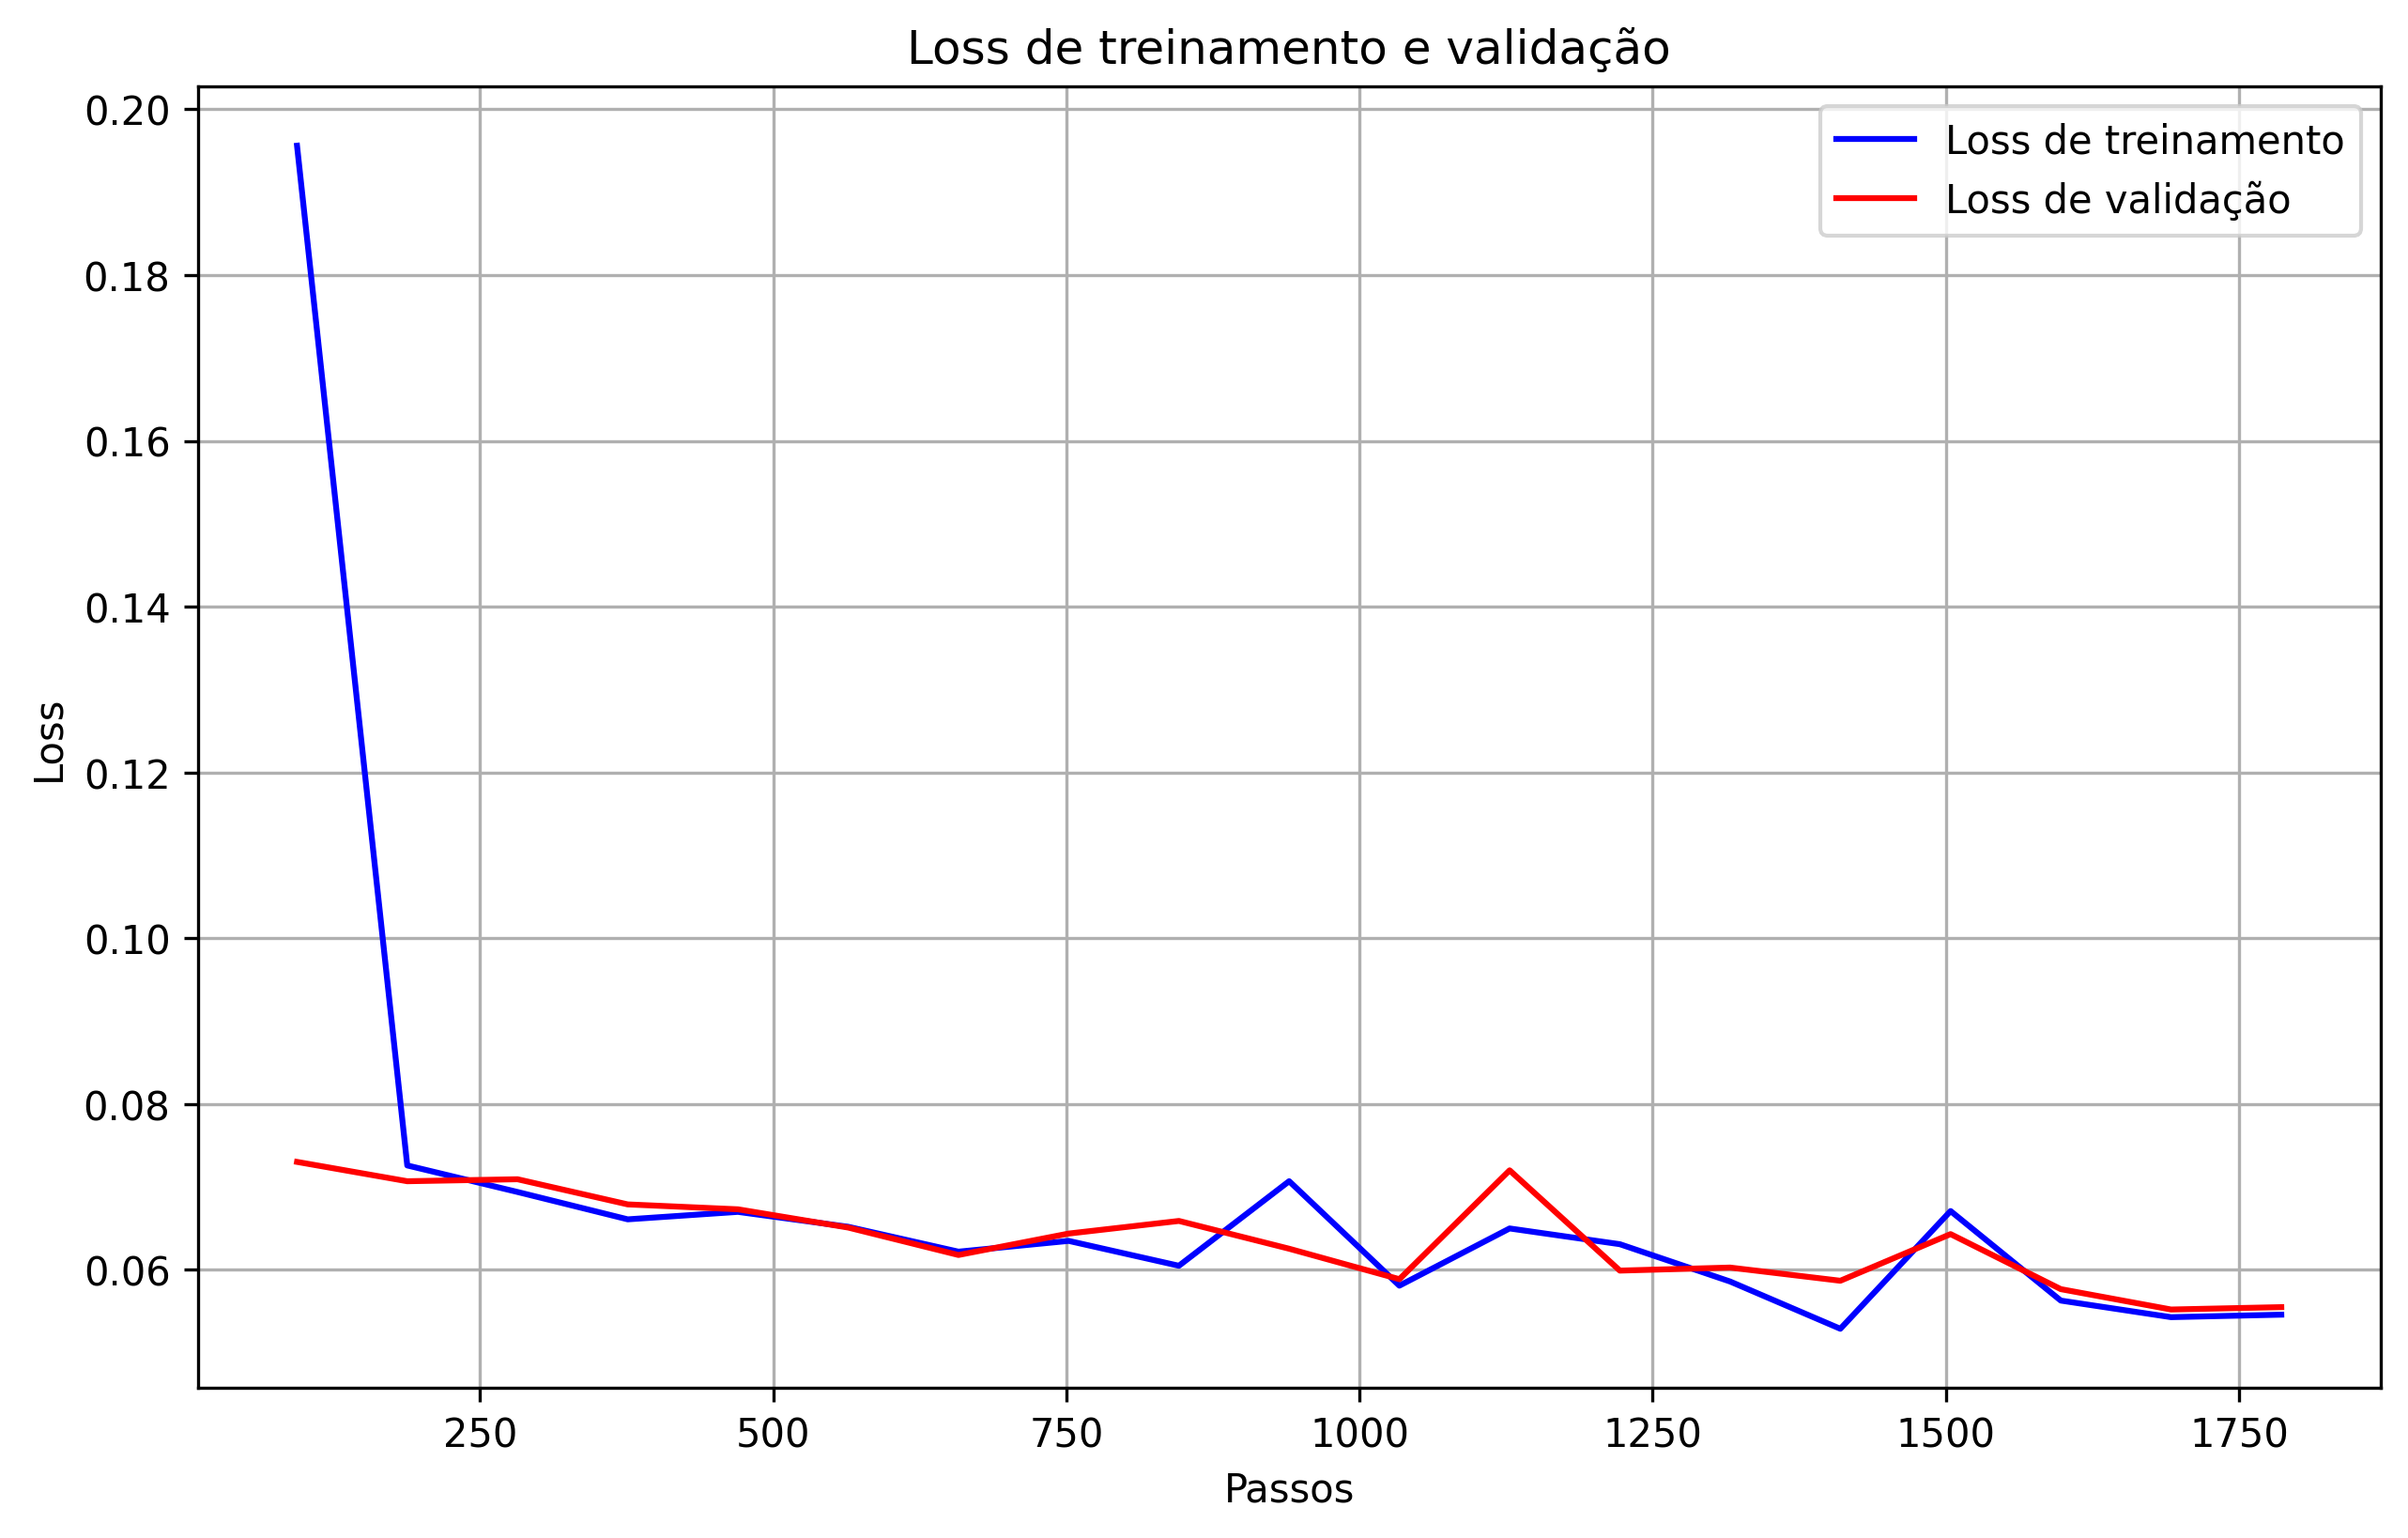
\includegraphics[width=0.725\columnwidth,keepaspectratio]{images/loss_qlora_5000.png}
    \label{fig:loss_qlora_5000}
    \fonte{Autoria própria.}
\end{figure}

\clearpage

\begin{figure}[ht]
    \centering
    \caption{\small \textit{Loss} de treinamento e validação para o \ac{LoRA} com 5000 amostras.}
    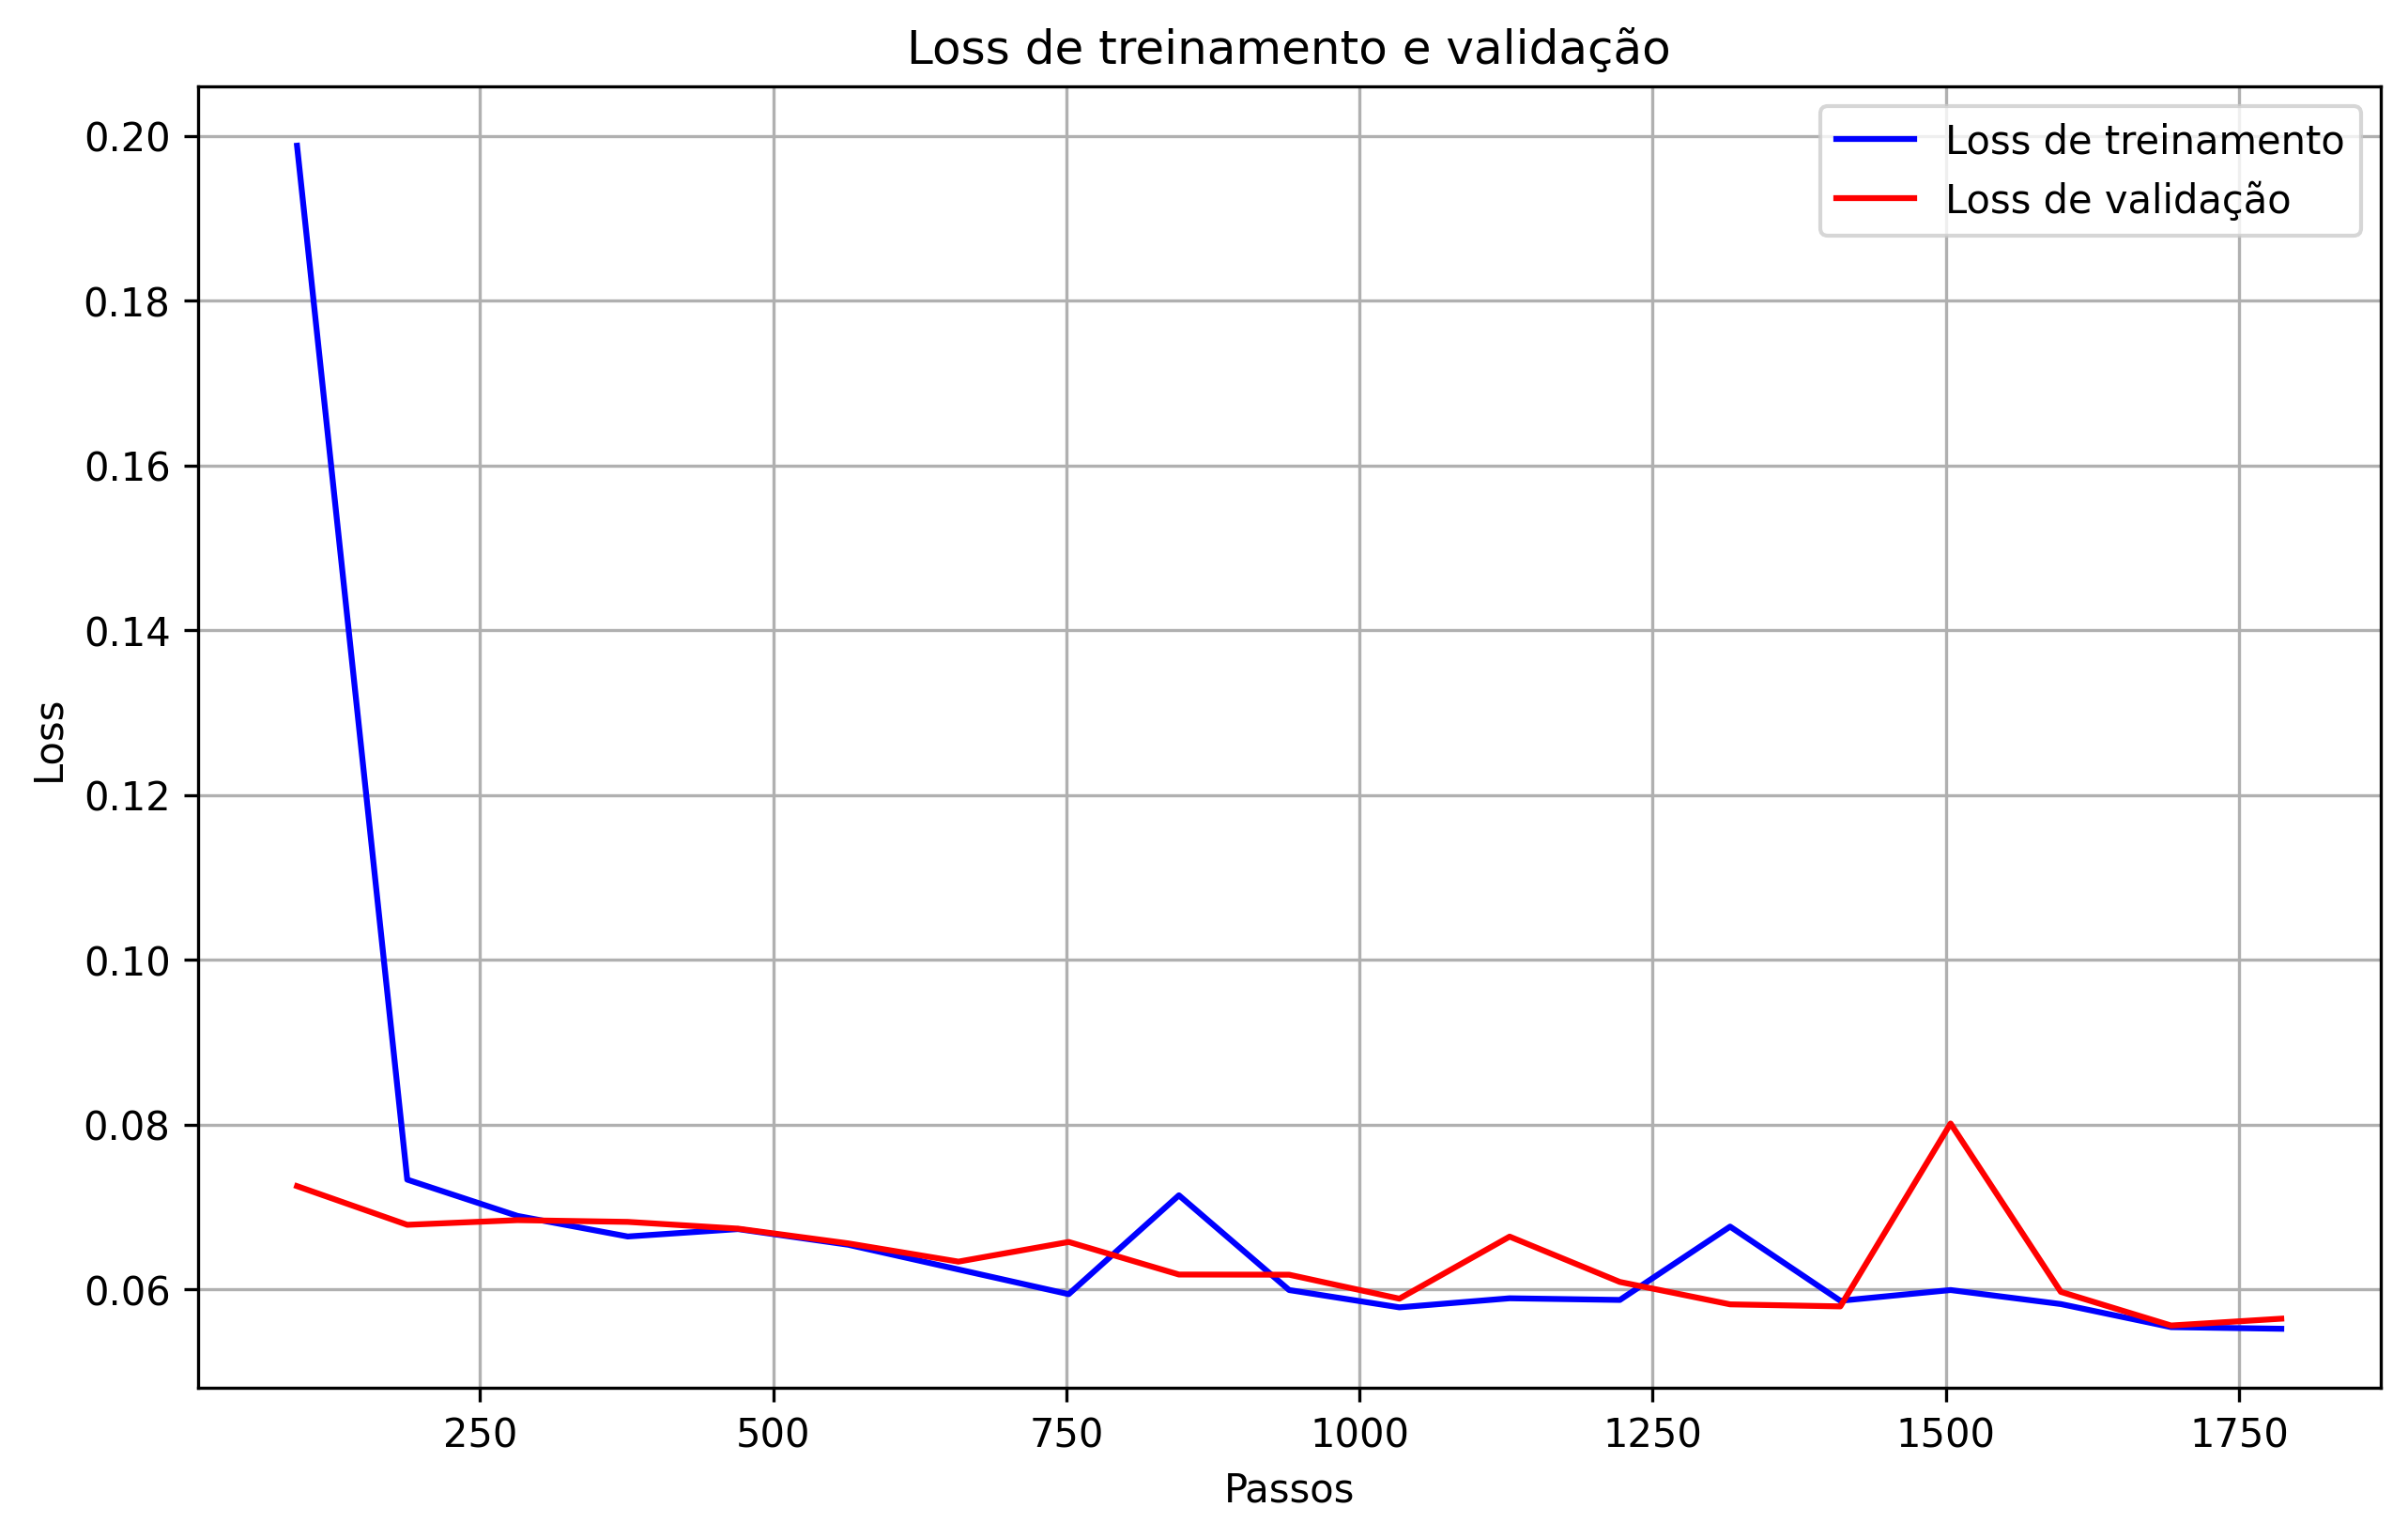
\includegraphics[width=0.725\columnwidth,keepaspectratio]{images/loss_lora_5000.png}
    \label{fig:loss_lora_5000}
    \fonte{Autoria própria.}
\end{figure}

\begin{figure}[ht]
    \centering
    \caption{\small \textit{Loss} de treinamento e validação para o \ac{QLoRA} com 9500 amostras.}
    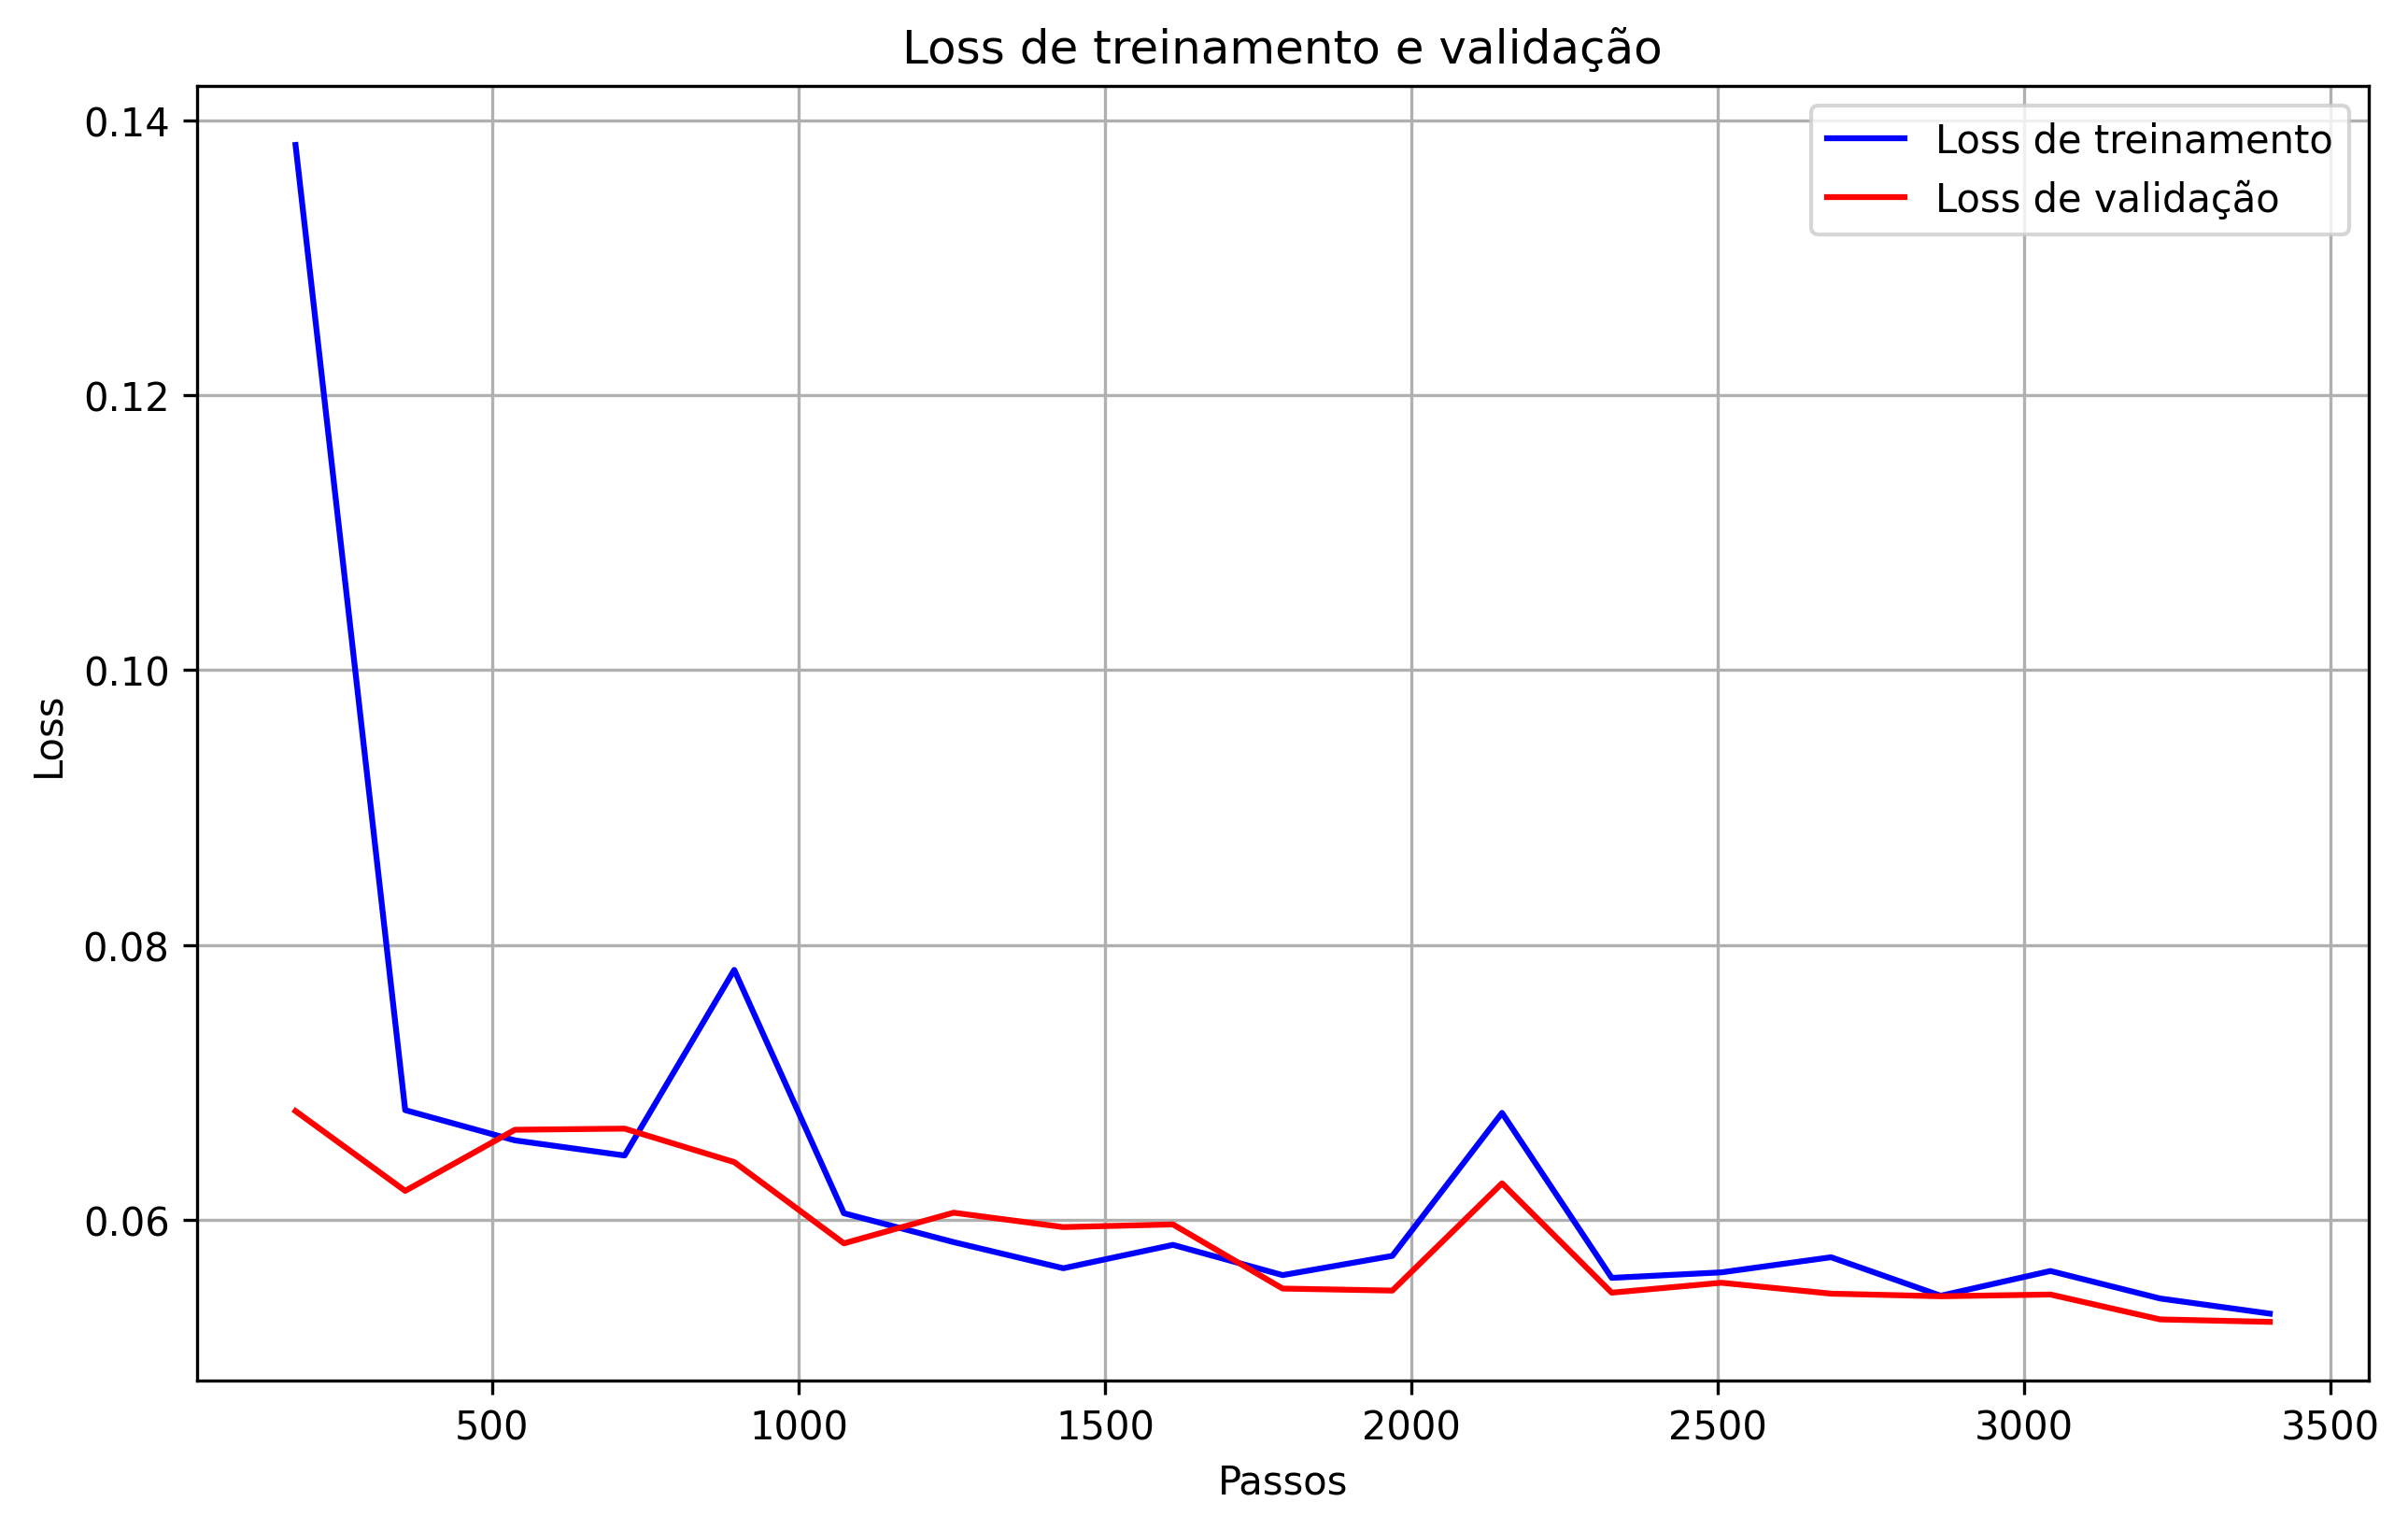
\includegraphics[width=0.725\columnwidth,keepaspectratio]{images/loss_qlora_9500.png}
    \label{fig:loss_qlora_9500}
    \fonte{Autoria própria.}
\end{figure}

\subsection{Análise dos treinamentos}

A vantagem no baixo gasto de memória do \ac{QLoRA} se torna evidente com os treinamentos, usando em média 1,8 vezes menos memória que o \ac{LoRA}. Observa-se também
que as configurações de \textit{fine-tuning} usadas no treinamento com 5000 e 9500 amostras levaram a uma maior instabilidade no \textit{loss} do longo dos passos.

\section{Testes}

Os testes se consistiram em uma série de perguntas aos modelos, em que foram usadas duas modalidades de pergunta, uma livre e outra objetiva. Na pergunta livre o
\textit{prompt} é definido como:

\begin{dialogue}
    \speak{Usuário} \textit{Classify the skin lesion in the image. \textbf{<imagem>}}
\end{dialogue}

Já na pergunta objetiva, é esperado que o modelo informe apenas o nome da doença com base nas opções possíveis do conjunto de dados, sendo que o \textit{prompt} usado é:

\begin{dialogue}
    \speak{Usuário} \textit{Classify the skin lesion in the image. Say only the name of the disease and nothing else. The diseases to be classified are: melanocytic Nevi,
        melanoma, benign keratosis-like lesions, basal cell carcinoma, actinic keratoses, vascular lesions and dermatofibroma.\textbf{<imagem>}}
\end{dialogue}

Foram feitas 100 perguntas livres e 1000 perguntas objetivass para cada modelo treinado e para o \ac{LLaMA}-3.2-11B-Vision-Instruct na versão normal e na quantizada. As
imagens utilizadas vieram da seção de teste do conjunto de dados. A \textit{temperatura}, uma variável que define a previsibilidade do modelo, foi definida como 0,1
para que as respostas fossem mais precisas. Além disso, o número máximo de \textit{tokens} foi definido como 128.

\section{Análise dos resultados parciais}

Os testes com perguntas livres foram avaliados manualmente para observar o formato de resposta dos modelos, enquanto os testes com perguntas objetivas foram processados
para a extração das lesões previstas para as imagens. Com esses dados, foram geradas matrizes de confusão com os cálculos da acurácia de cada modelo.

\subsection{Análise do LLaMA-3.2-Vision-Instruct}

Tanto o modelo na versão normal quanto o modelo quantizado apresentaram respostas bem variadas para cada pergunta livre. Em geral, as respostas apresentam uma estrutura
de passos que se baseia em metodologias de classificação de lesões de pele. O diálogo abaixo apresenta uma classificação correta para a imagem de um melanoma:

\begin{dialogue}
    \speak{Usuário} \textit{Classify the skin lesion in the image. \textbf{<imagem de um melanoma>}} \\
    \speak{Modelo} \textit{\textbf{Step 1: Identify the lesion.} \\
        The image shows a skin lesion with an irregular border and a dark brown color. \\
        \textbf{Step 2: Determine the characteristics of the lesion.} \\
        The lesion has an irregular border, which is a characteristic of melanoma. The dark brown color is also consistent with melanoma. \\
        \textbf{Step 3: Consider the possible diagnoses.} \\
        Based on the characteristics of the lesion, it is likely that the diagnosis is melanoma. \\
        \textbf{Step 4: Provide the final answer.} \\
        \textbf{Answer:} Melanoma}
\end{dialogue}

Muitas respostas apresentaram uma classificação incorreta, embora tenham sido descritivas sobre a lesão. No exemplo abaixo, o modelo classificou um nevo melanocítico
como um melanoma:

\begin{dialogue}
    \speak{Usuário} \textit{Classify the skin lesion in the image. \textbf{<imagem de um nevo melanocítico>}} \\
    \speak{Modelo} \textit{\textbf{Step 1: Identify the lesion} \\
        The image shows a brown, irregularly shaped lesion with a darker brown border. \\
        \textbf{Step 2: Determine the characteristics of the lesion} \\
        The lesion is asymmetrical, has an irregular border, and has multiple colors. \\
        \textbf{Step 3: Classify the lesion} \\
        Based on the characteristics of the lesion, it is classified as a melanoma. \\
        \textbf{Answer:} Melanoma}
\end{dialogue}

Algumas respostas não apresentaram uma classificação precisa, sendo que o modelo informou apenas que a imagem se tratava de uma lesão de pele. Um exemplo assim pode ser
visto no diálogo abaixo:

\begin{dialogue}
    \speak{Usuário} \textit{Classify the skin lesion in the image. \textbf{<imagem de um nevo melanocítico>}} \\
    \speak{Modelo} \textit{The skin lesion in the image appears to be a dermatological condition, likely a typeof skin cancer or a benign growth. However, without
        further information or a medical diagnosis, it is difficult to provide a definitive classification.}
\end{dialogue}

Já nas respostas às perguntas objetivas, o modelo quantizado teve um desempenho levemente pior em relação ao não quantizado. Porém, ambos tiveram um desempenho pouco
satisfatório, a versão quantizada atingiu apenas 11,8\% de acurácia e a não quantizada atingiu 14\%.

A \autoref{fig:confusion_matrix_llama_quantized} e a \autoref{fig:confusion_matrix_llama} apresentam as matrizes de confusão normalizadas pelos valores verdadeiros para
o modelo quantizado e o não quantizado, respectivamente. Nota-se que eles classificaram as lesões como melanoma em uma escala desproporcional, o \ac{LLaMA} quantizado
classificou 97,6\% das lesões como melanoma, enquanto o não quantizado classificou 88,3\%. Também pode-se notar uma tendência da classificação de lesões vasculares como
dermatofibroma por parte do modelo não quantizado.

Foram registradas 3 respostas incertas para o modelo quantizado e apenas uma para o não quantizado.

\begin{figure}[ht]
    \centering
    \caption{\small Matriz de confusão para o \ac{LLaMA}-11B-Vision-Instruct quantizado.}
    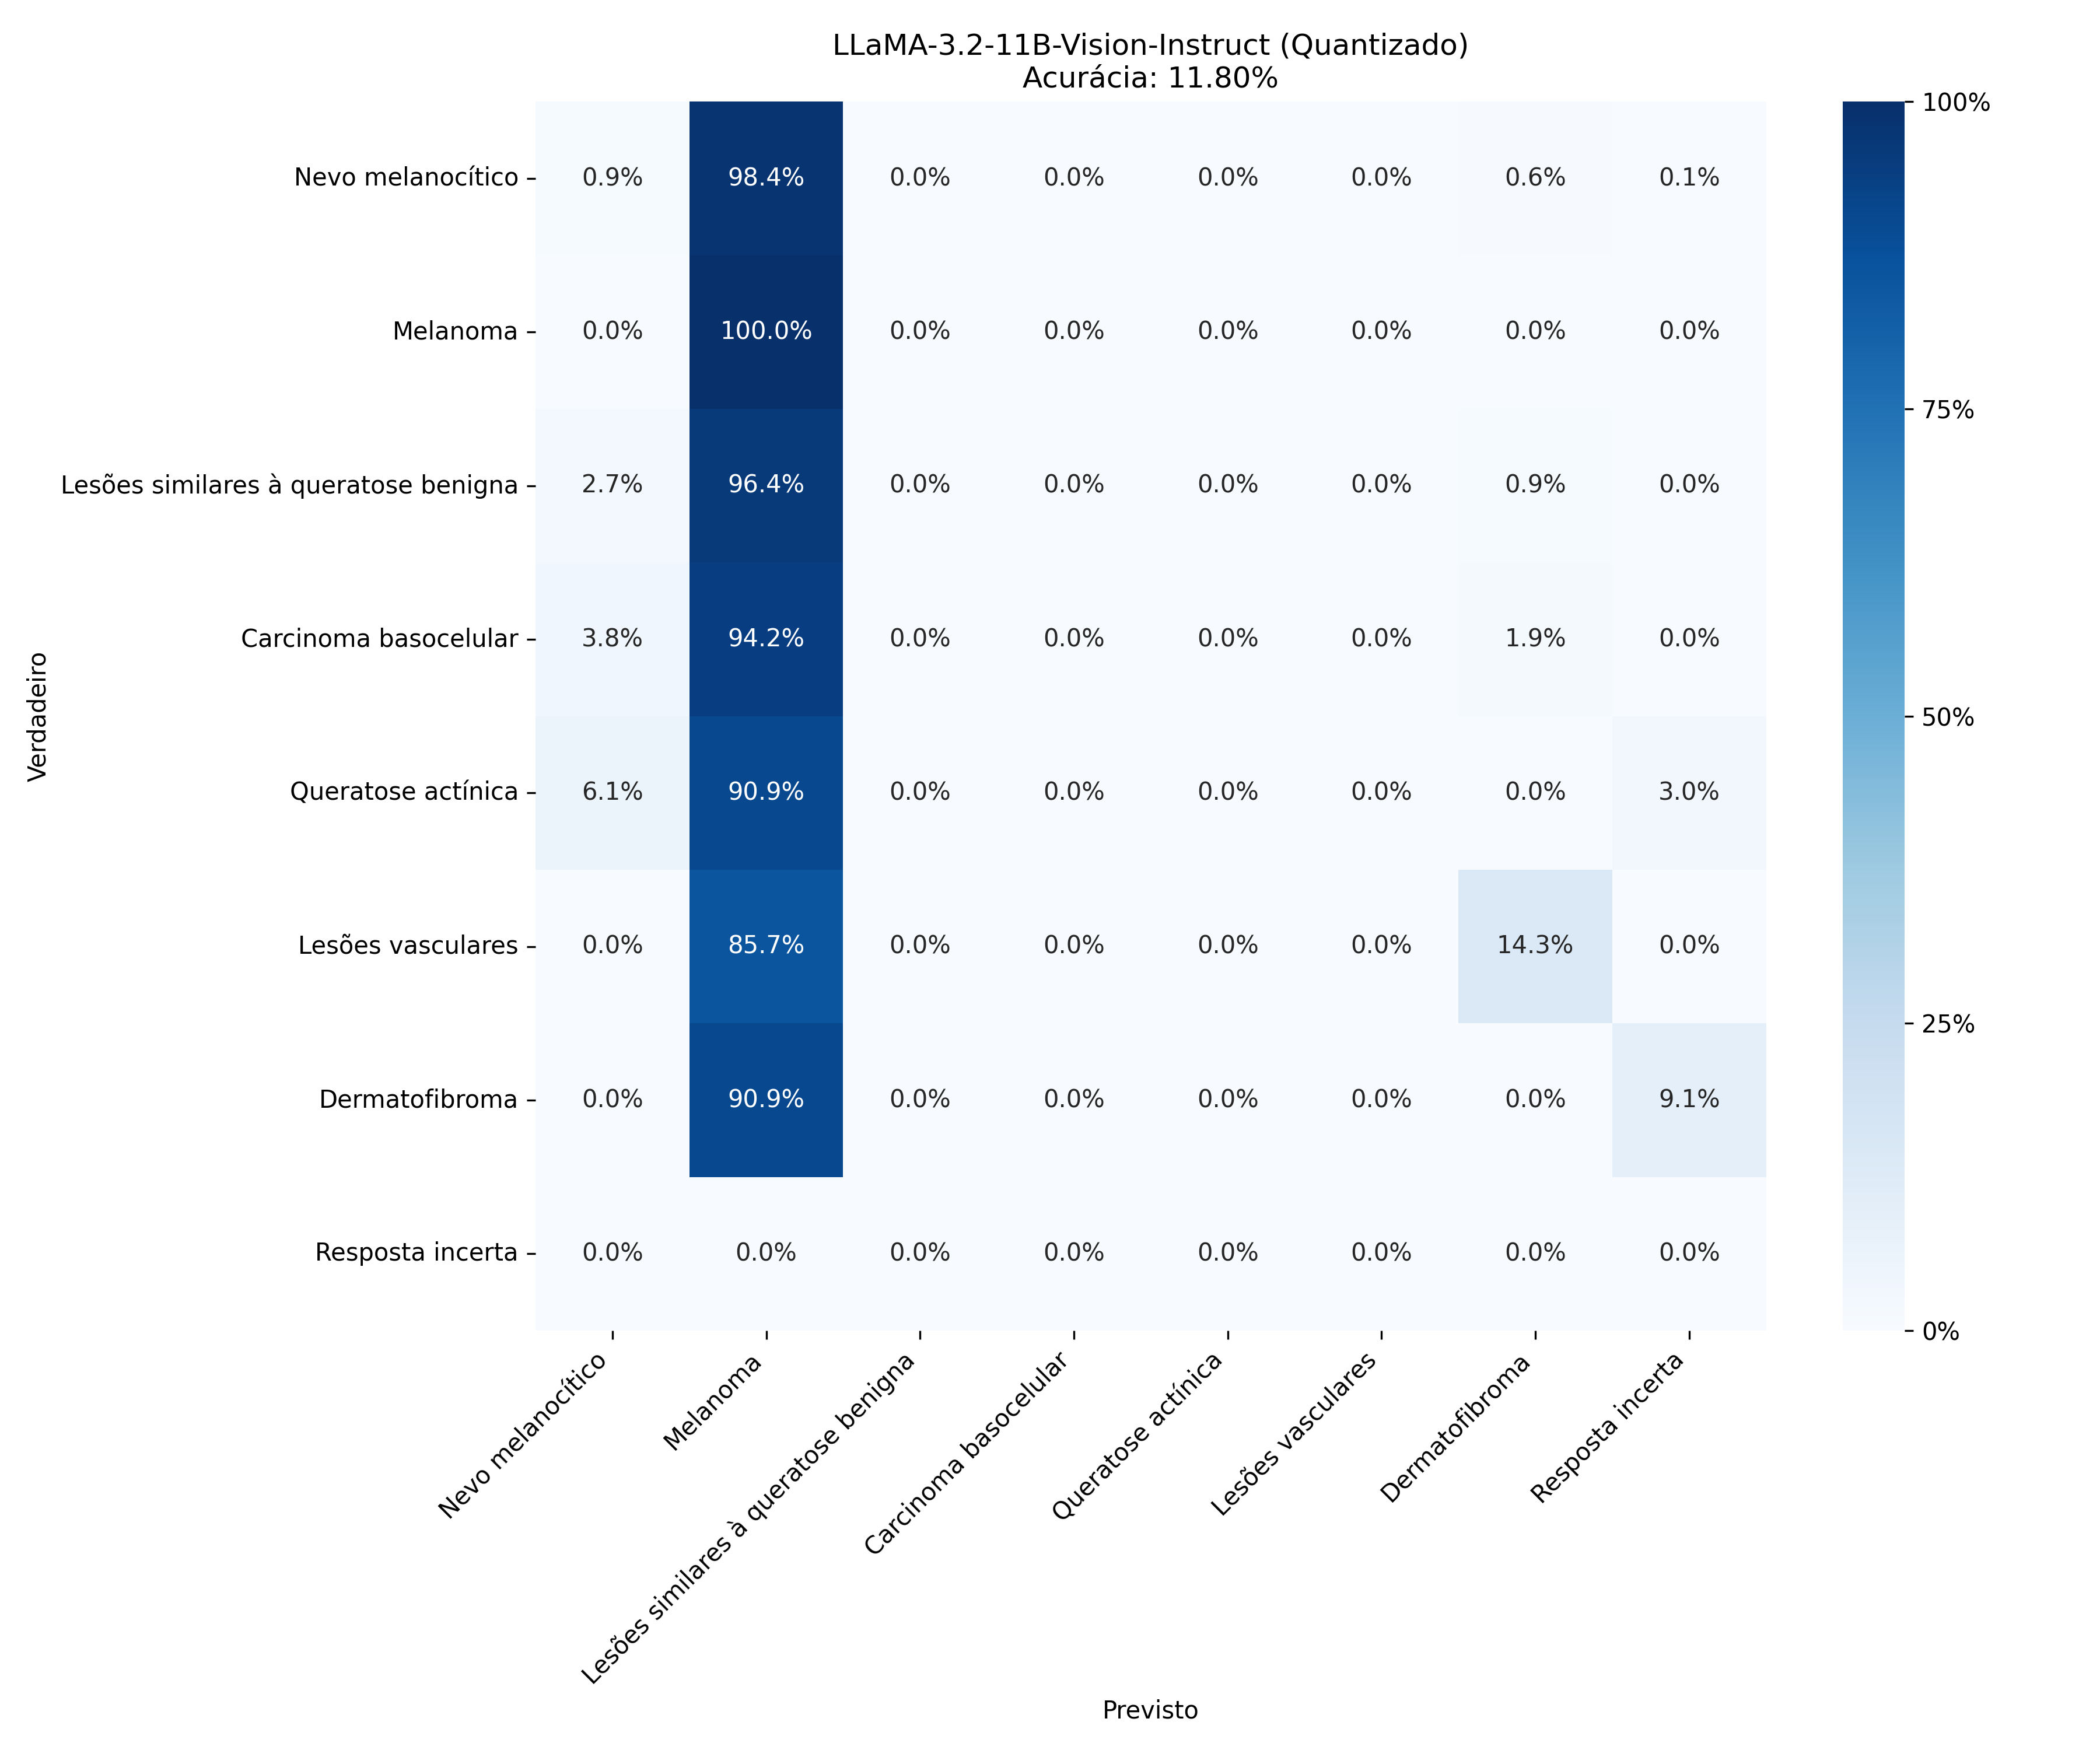
\includegraphics[width=1\columnwidth,keepaspectratio]{images/confusion_matrix_llama_3.2_11b_vision_instruct_quantized.png}
    \label{fig:confusion_matrix_llama_quantized}
    \fonte{Autoria própria.}
\end{figure}

\clearpage

\begin{figure}[ht]
    \centering
    \caption{\small Matriz de confusão para o \ac{LLaMA}-11B-Vision-Instruct.}
    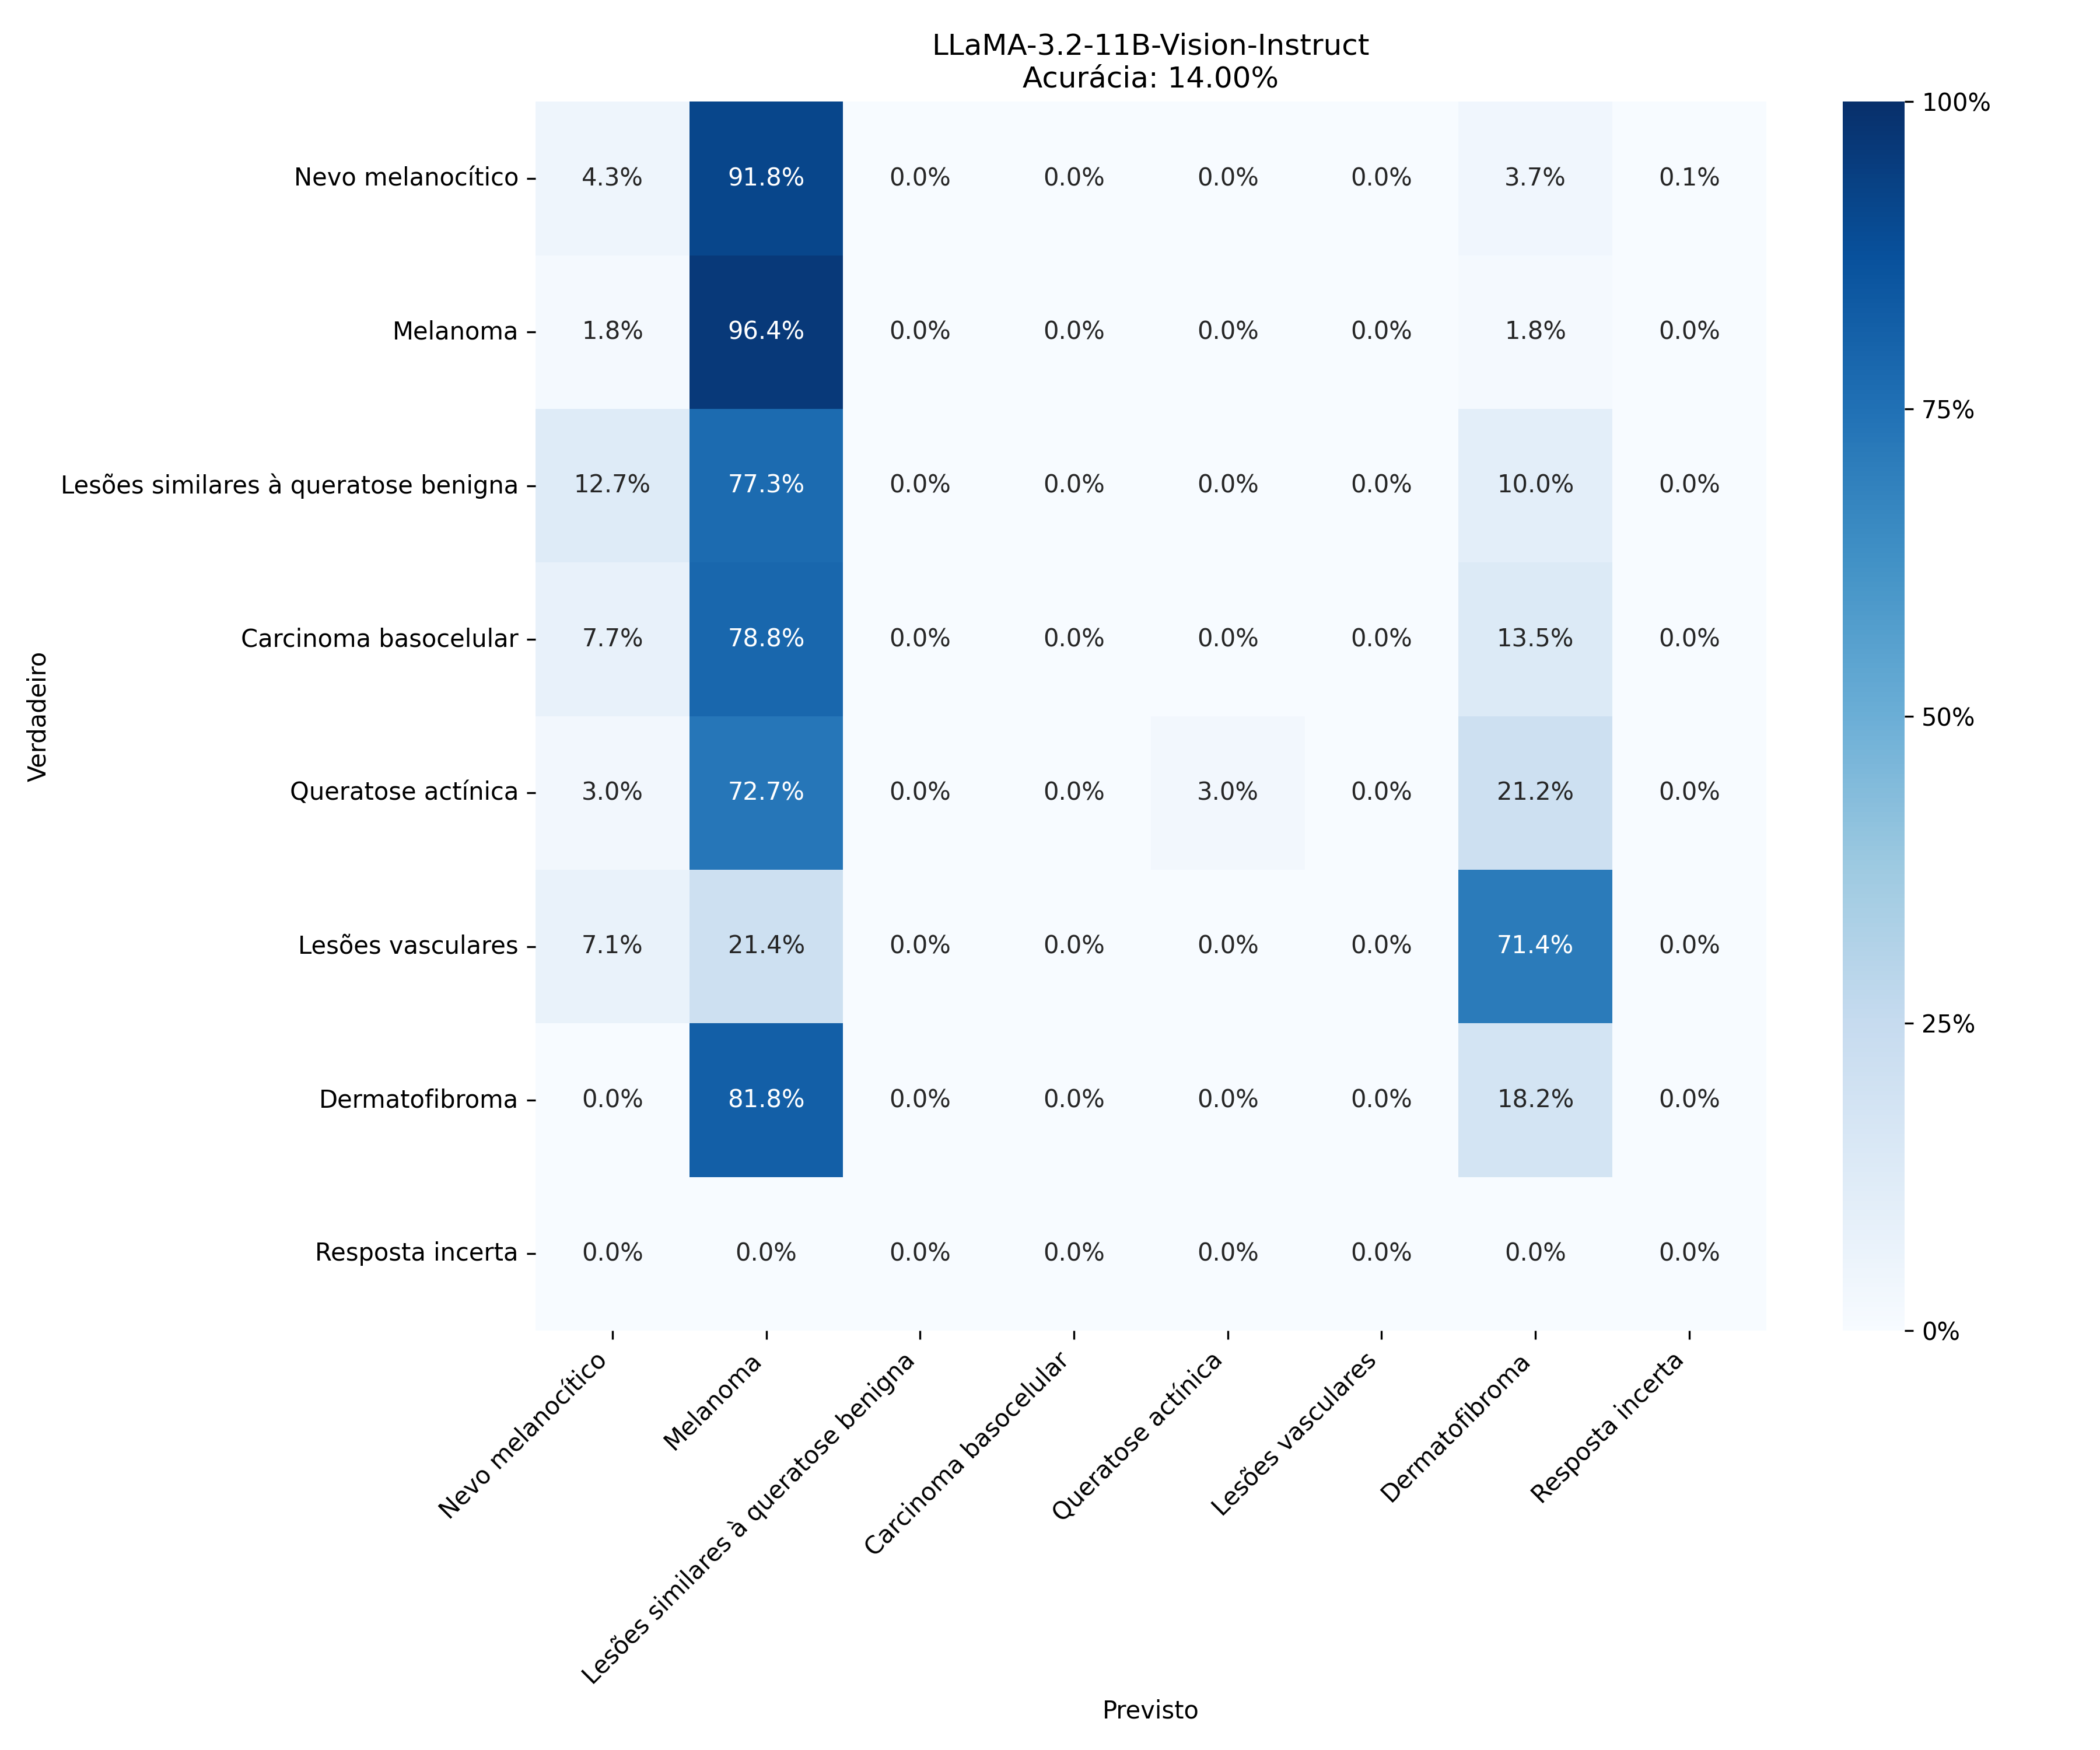
\includegraphics[width=1\columnwidth,keepaspectratio]{images/confusion_matrix_llama_3.2_11b_vision_instruct.png}
    \label{fig:confusion_matrix_llama}
    \fonte{Autoria própria.}
\end{figure}

\subsection{Análise dos modelos após o \textit{fine-tuning}}

Para as perguntas livres, todos os modelos treinados responderam no formato especificado no treinamento. O primeiro diálogo abaixo apresenta uma classificação correta e
o segundo apresenta uma incorreta, ambas as respostas foram dadas pelo modelo treinado com \ac{QLoRA} com 450 amostras:

\begin{dialogue}
    \speak{Usuário} \textit{Classify the skin lesion in the image. \textbf{<imagem de um nevo melanocítico>}} \\
    \speak{Modelo} \textit{The skin lesion in the image is melanocytic Nevi.}
\end{dialogue}

\begin{dialogue}
    \speak{Usuário} \textit{Classify the skin lesion in the image. \textbf{<imagem de um nevo melanoma>}} \\
    \speak{Modelo} \textit{The skin lesion in the image is benign keratosis-like lesions.}
\end{dialogue}

Os modelos trainados com \ac{QLoRA} com 450, 5000 e 9500 amostras, e com \ac{LoRA} com 5000 amostras apresentaram um problema em que as respostas não obedecem ao formato
especificado na pergunta objetiva, respondendo com o texto completo.

A acurácia nas respostas às perguntas objetivas aumentou consideravelmente com o \textit{fine-tuning} com \ac{QLoRA}, chegando a atingir 65,5\%. Porém, o modelo gerado
com esse treinamento tende a classificar a maioria das lesões como nevo melanocítico, o que indica que a acurácia maior pode ser simplesmente devido a uma quantidade
maior de nevos melanocíticos nos dados de teste. Para o modelo treinado com \ac{LoRA}, o desempenho foi menor, atingindo apenas 49,5\% de acurácia.

Em geral, como pode ser visto na \autoref{fig:confusion_matrix_qlora_450} e \autoref{fig:confusion_matrix_lora_450}, as duas versões ficaram insatisfatórias, o que se
deve a um treinamento com um conjunto pequeno de dados e hiperparâmetros não ideais.

\begin{figure}[ht]
    \centering
    \caption{\small Matriz de confusão para o \ac{LLaMA} treinado com \ac{QLoRA} e 450 amostras.}
    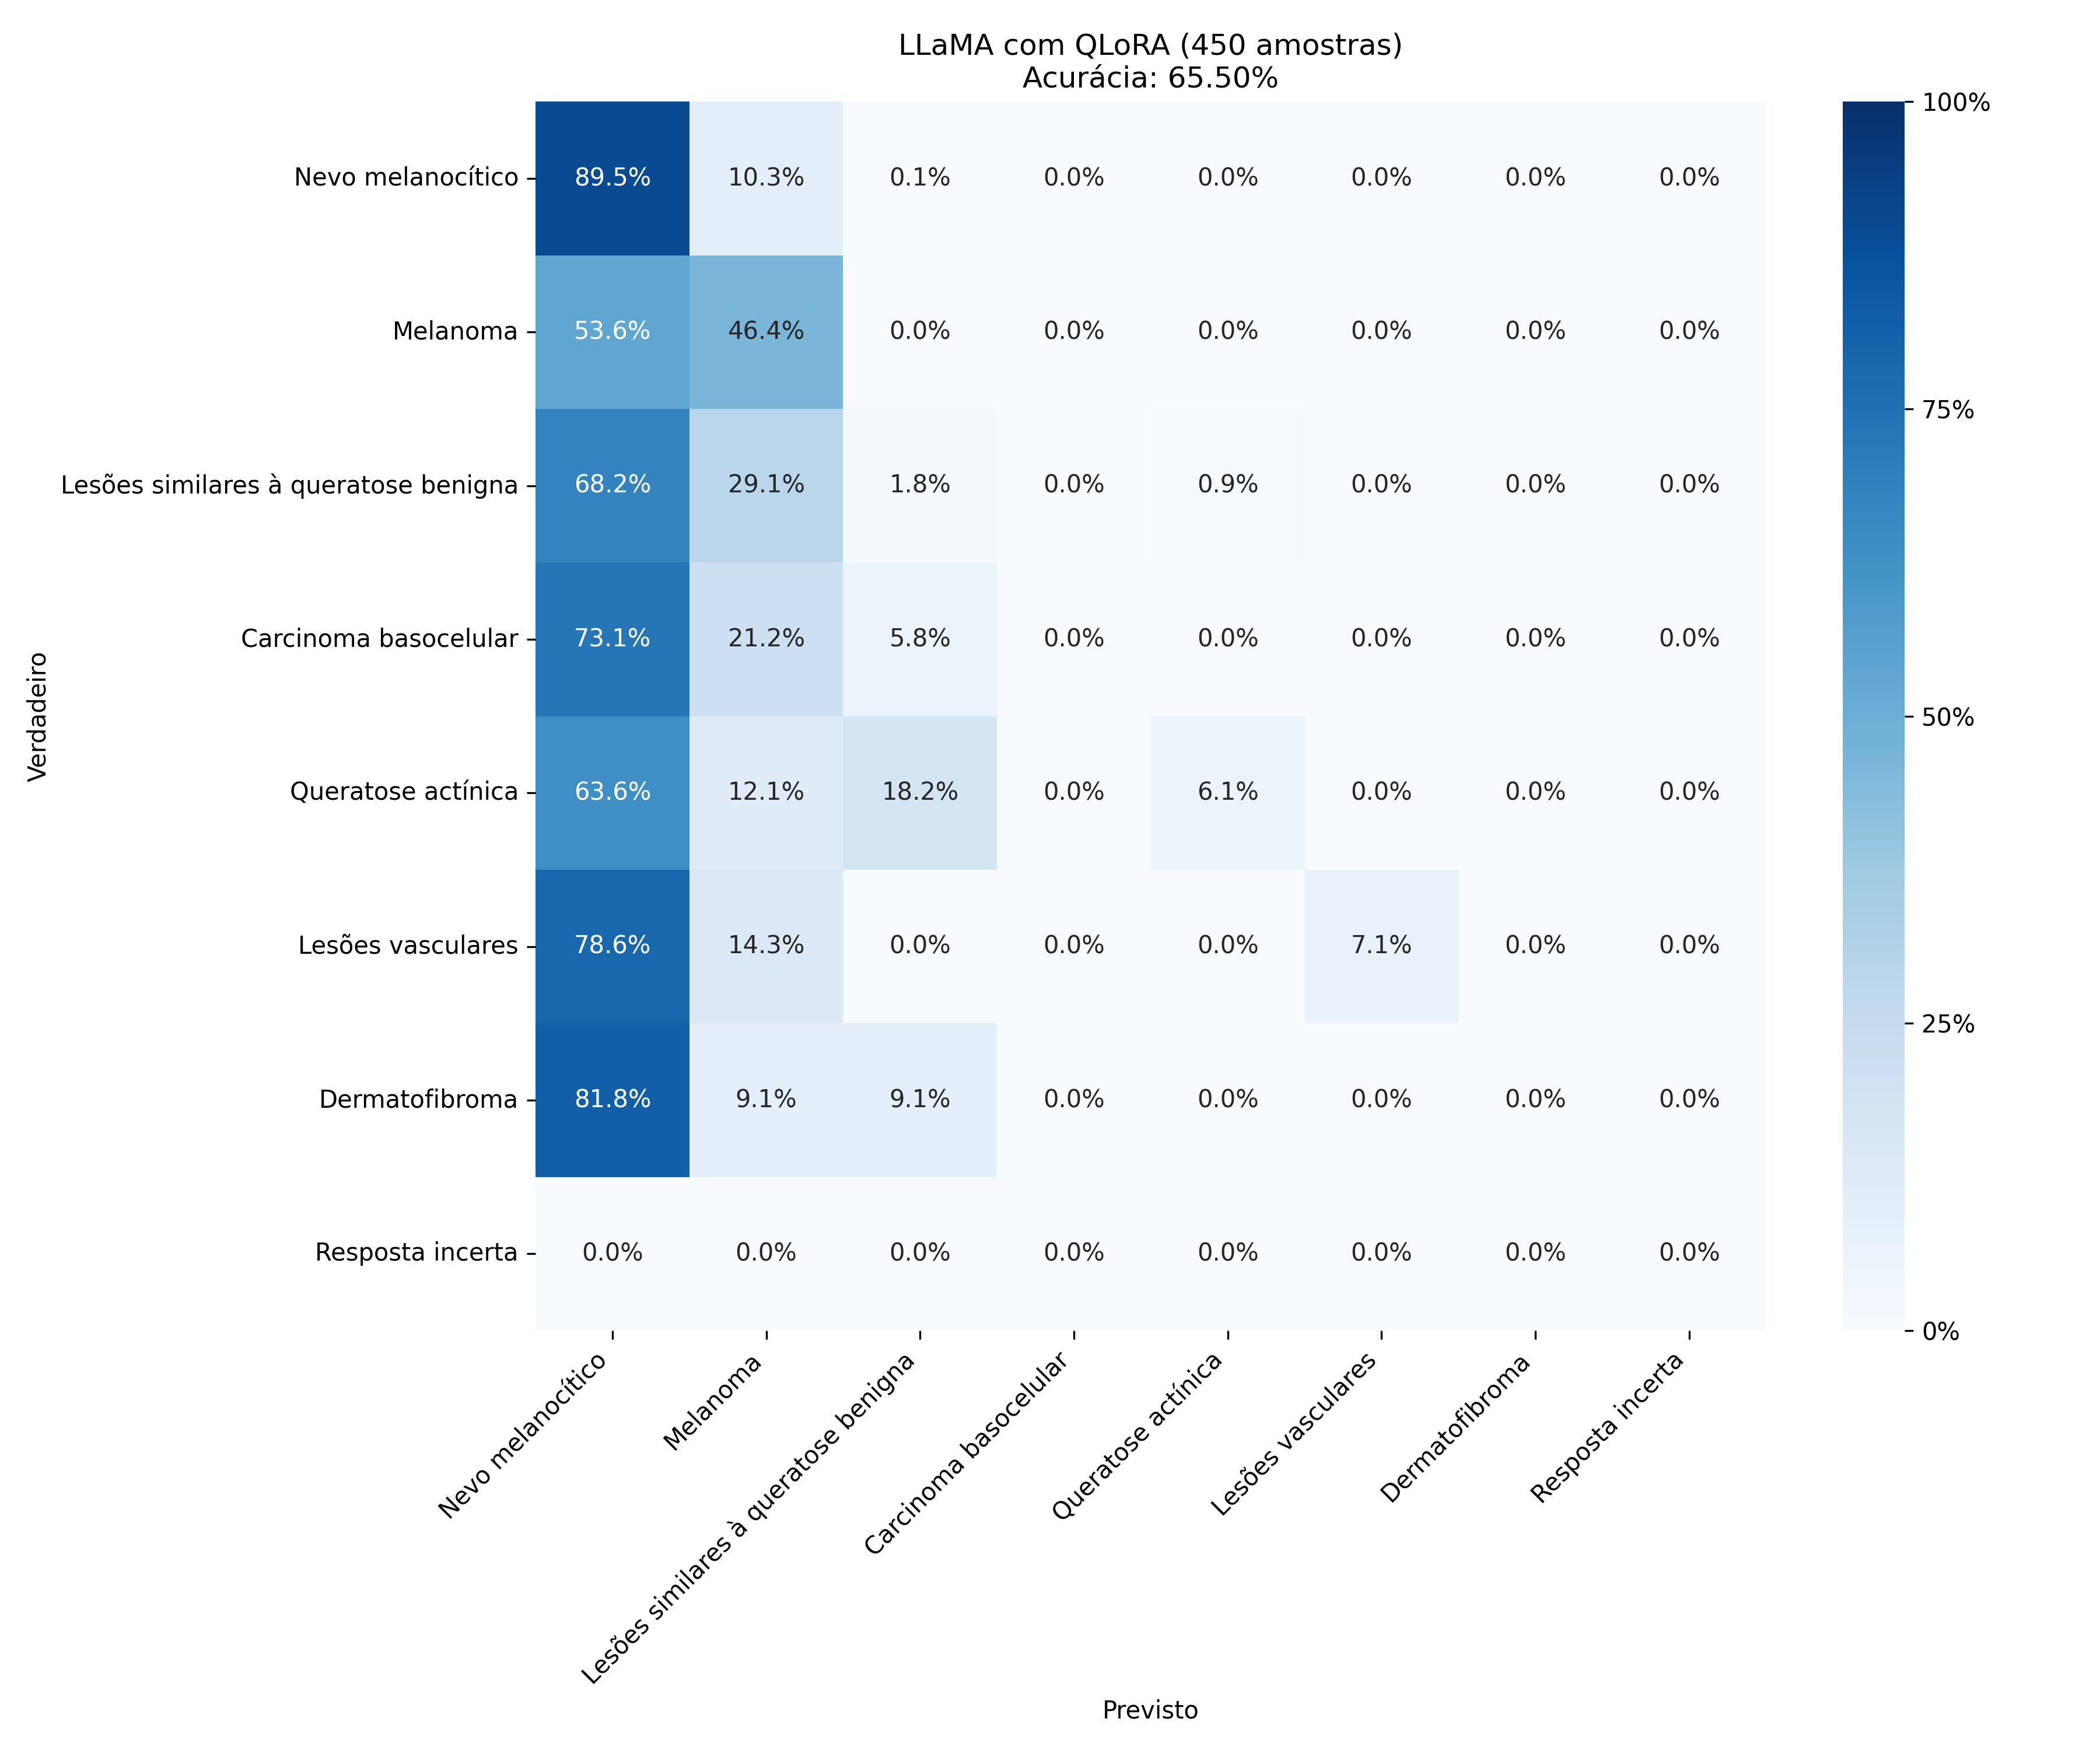
\includegraphics[width=1\columnwidth,keepaspectratio]{images/confusion_matrix_qlora_450.png}
    \label{fig:confusion_matrix_qlora_450}
    \fonte{Autoria própria.}
\end{figure}

\clearpage

\begin{figure}[ht]
    \centering
    \caption{\small Matriz de confusão para o \ac{LLaMA} treinado com \ac{LoRA} e 450 amostras.}
    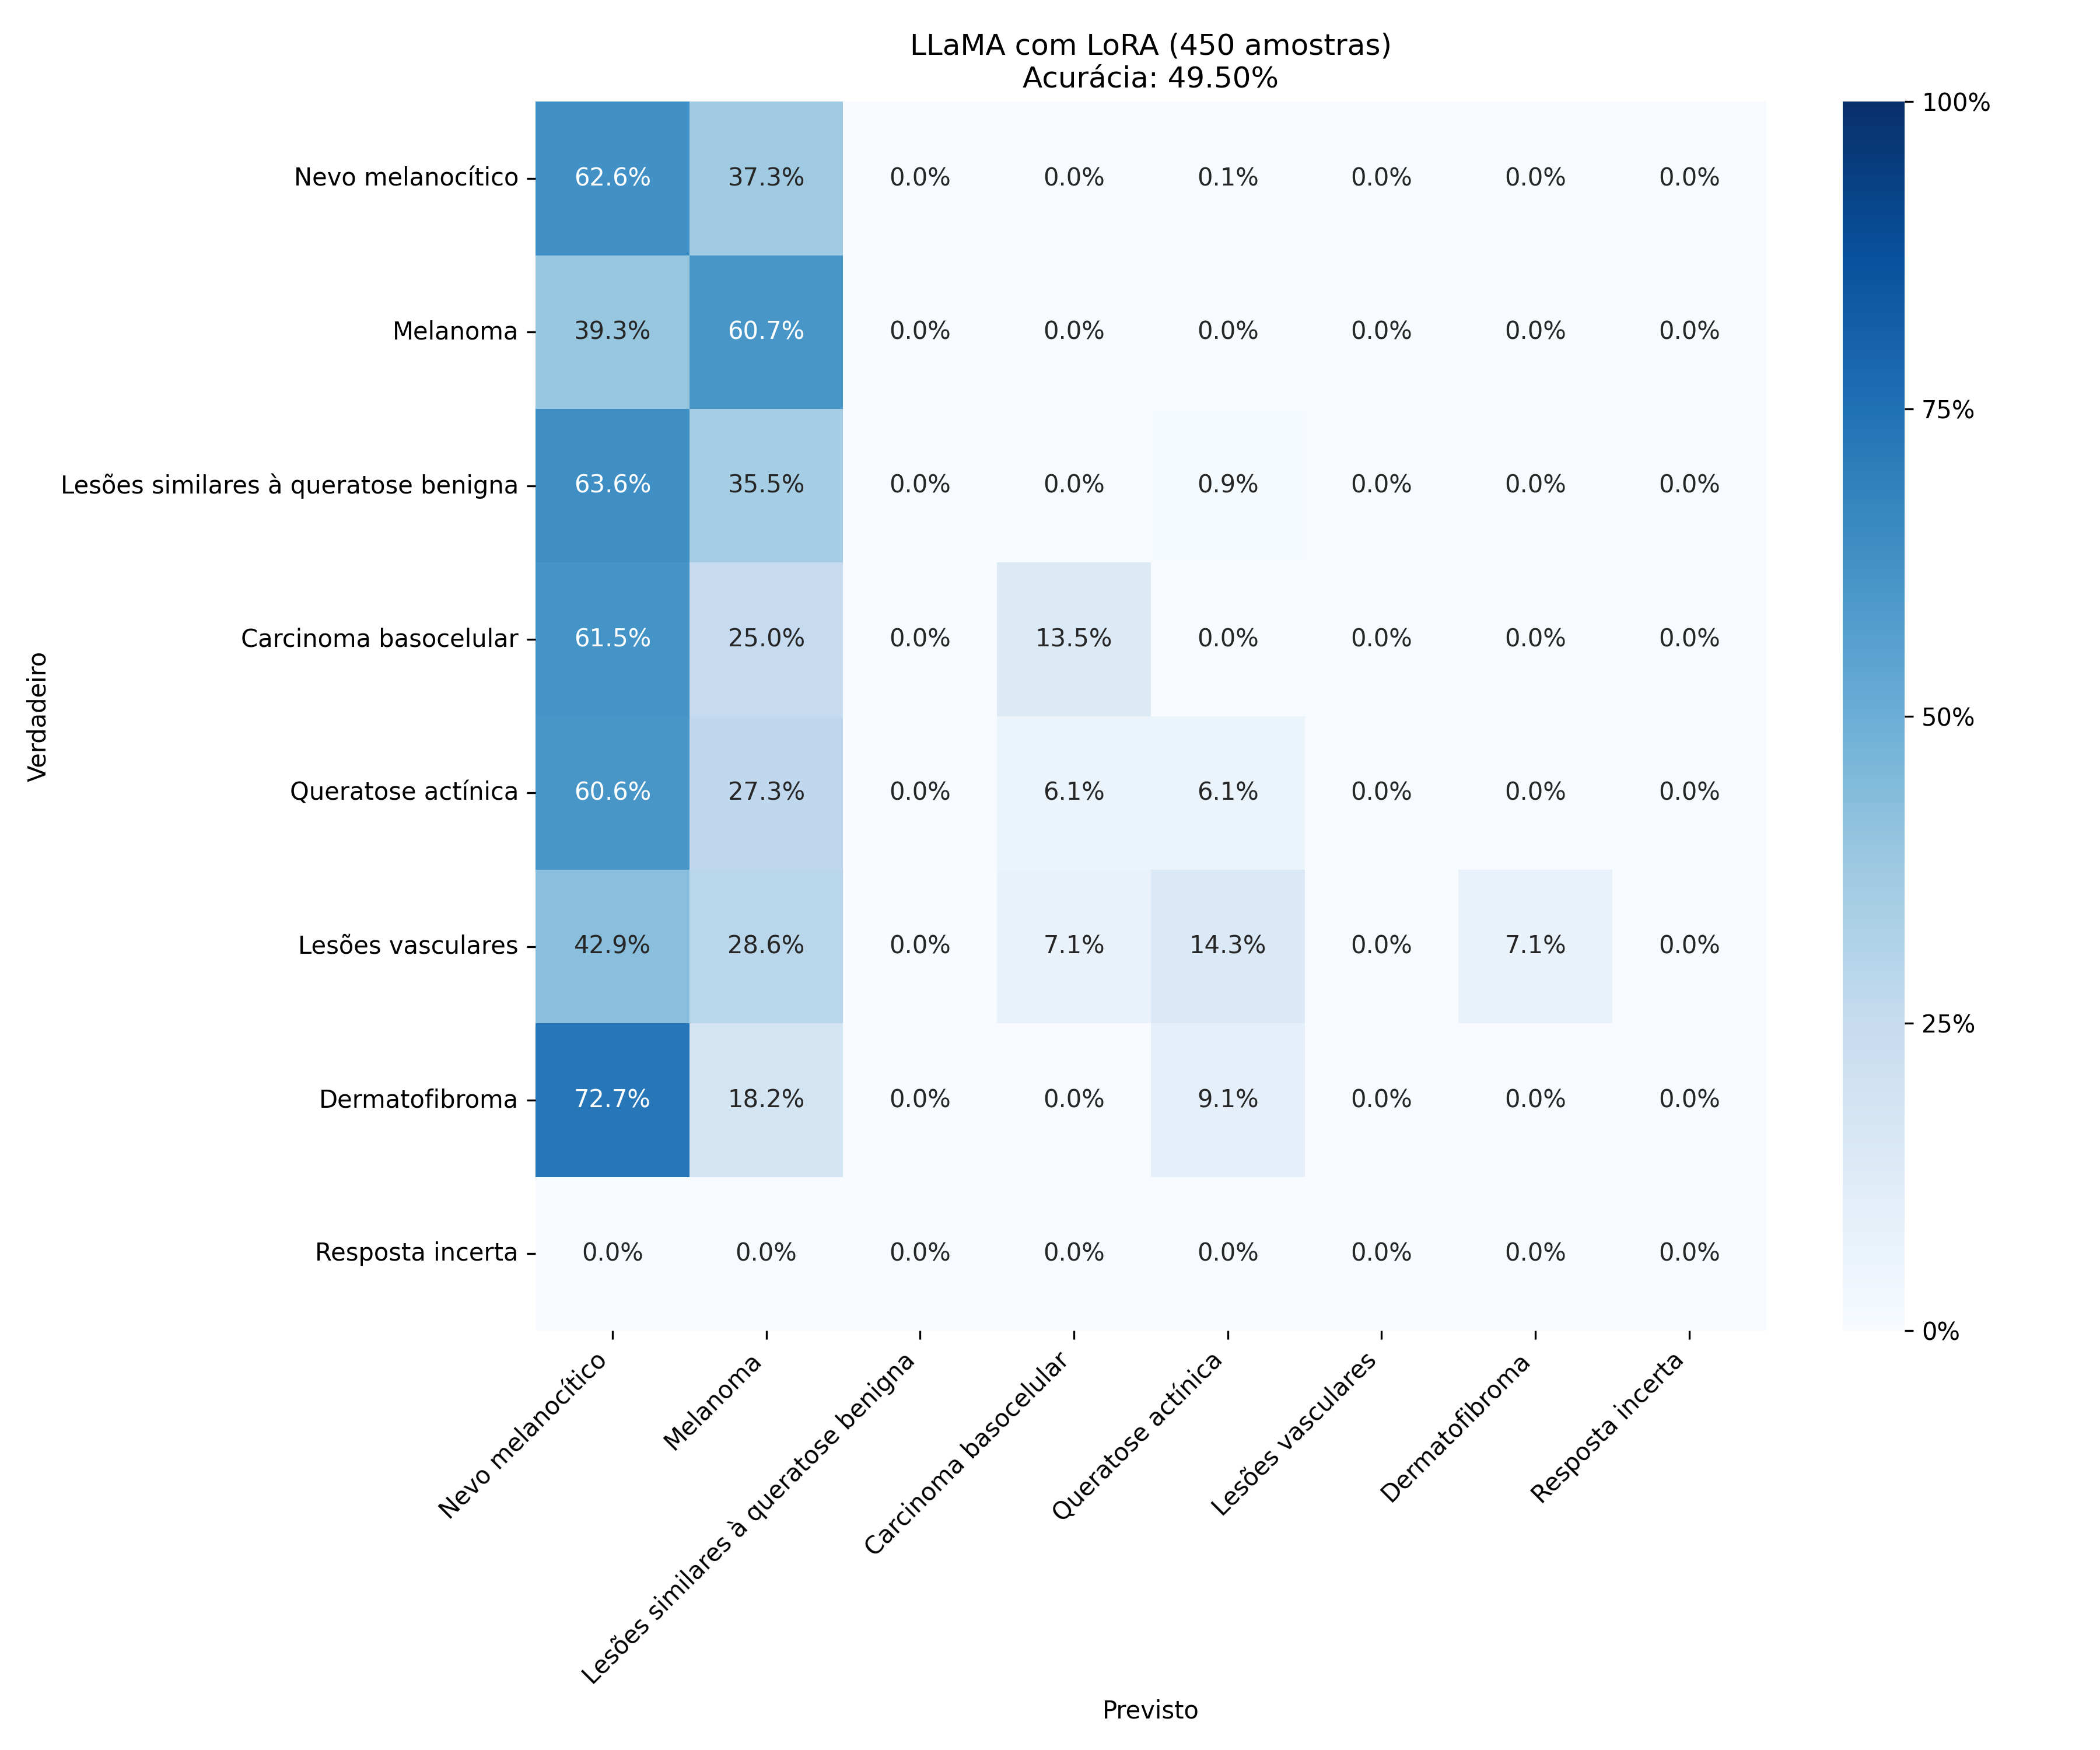
\includegraphics[width=1\columnwidth,keepaspectratio]{images/confusion_matrix_lora_450.png}
    \label{fig:confusion_matrix_lora_450}
    \fonte{Autoria própria.}
\end{figure}

A acurácia decaiu levemente no \textit{fine-tuning} com 900 amostas, conforme apresentado na \autoref{fig:confusion_matrix_qlora_900} e
\autoref{fig:confusion_matrix_lora_900}, ficando em 65.2\% para o \ac{LLaMA} treinado com \ac{QLoRA} e 42\% para o treinado com \ac{LoRA}. Porém, o modelo treinado com
\ac{QLoRA} apresenta um padrão melhor de classificação, reconhecendo melhor as lesões de nevos melanocíticos e de queratoses actínicas.

\clearpage

\begin{figure}[ht]
    \centering
    \caption{\small Matriz de confusão para o \ac{LLaMA} treinado com \ac{QLoRA} e 900 amostras.}
    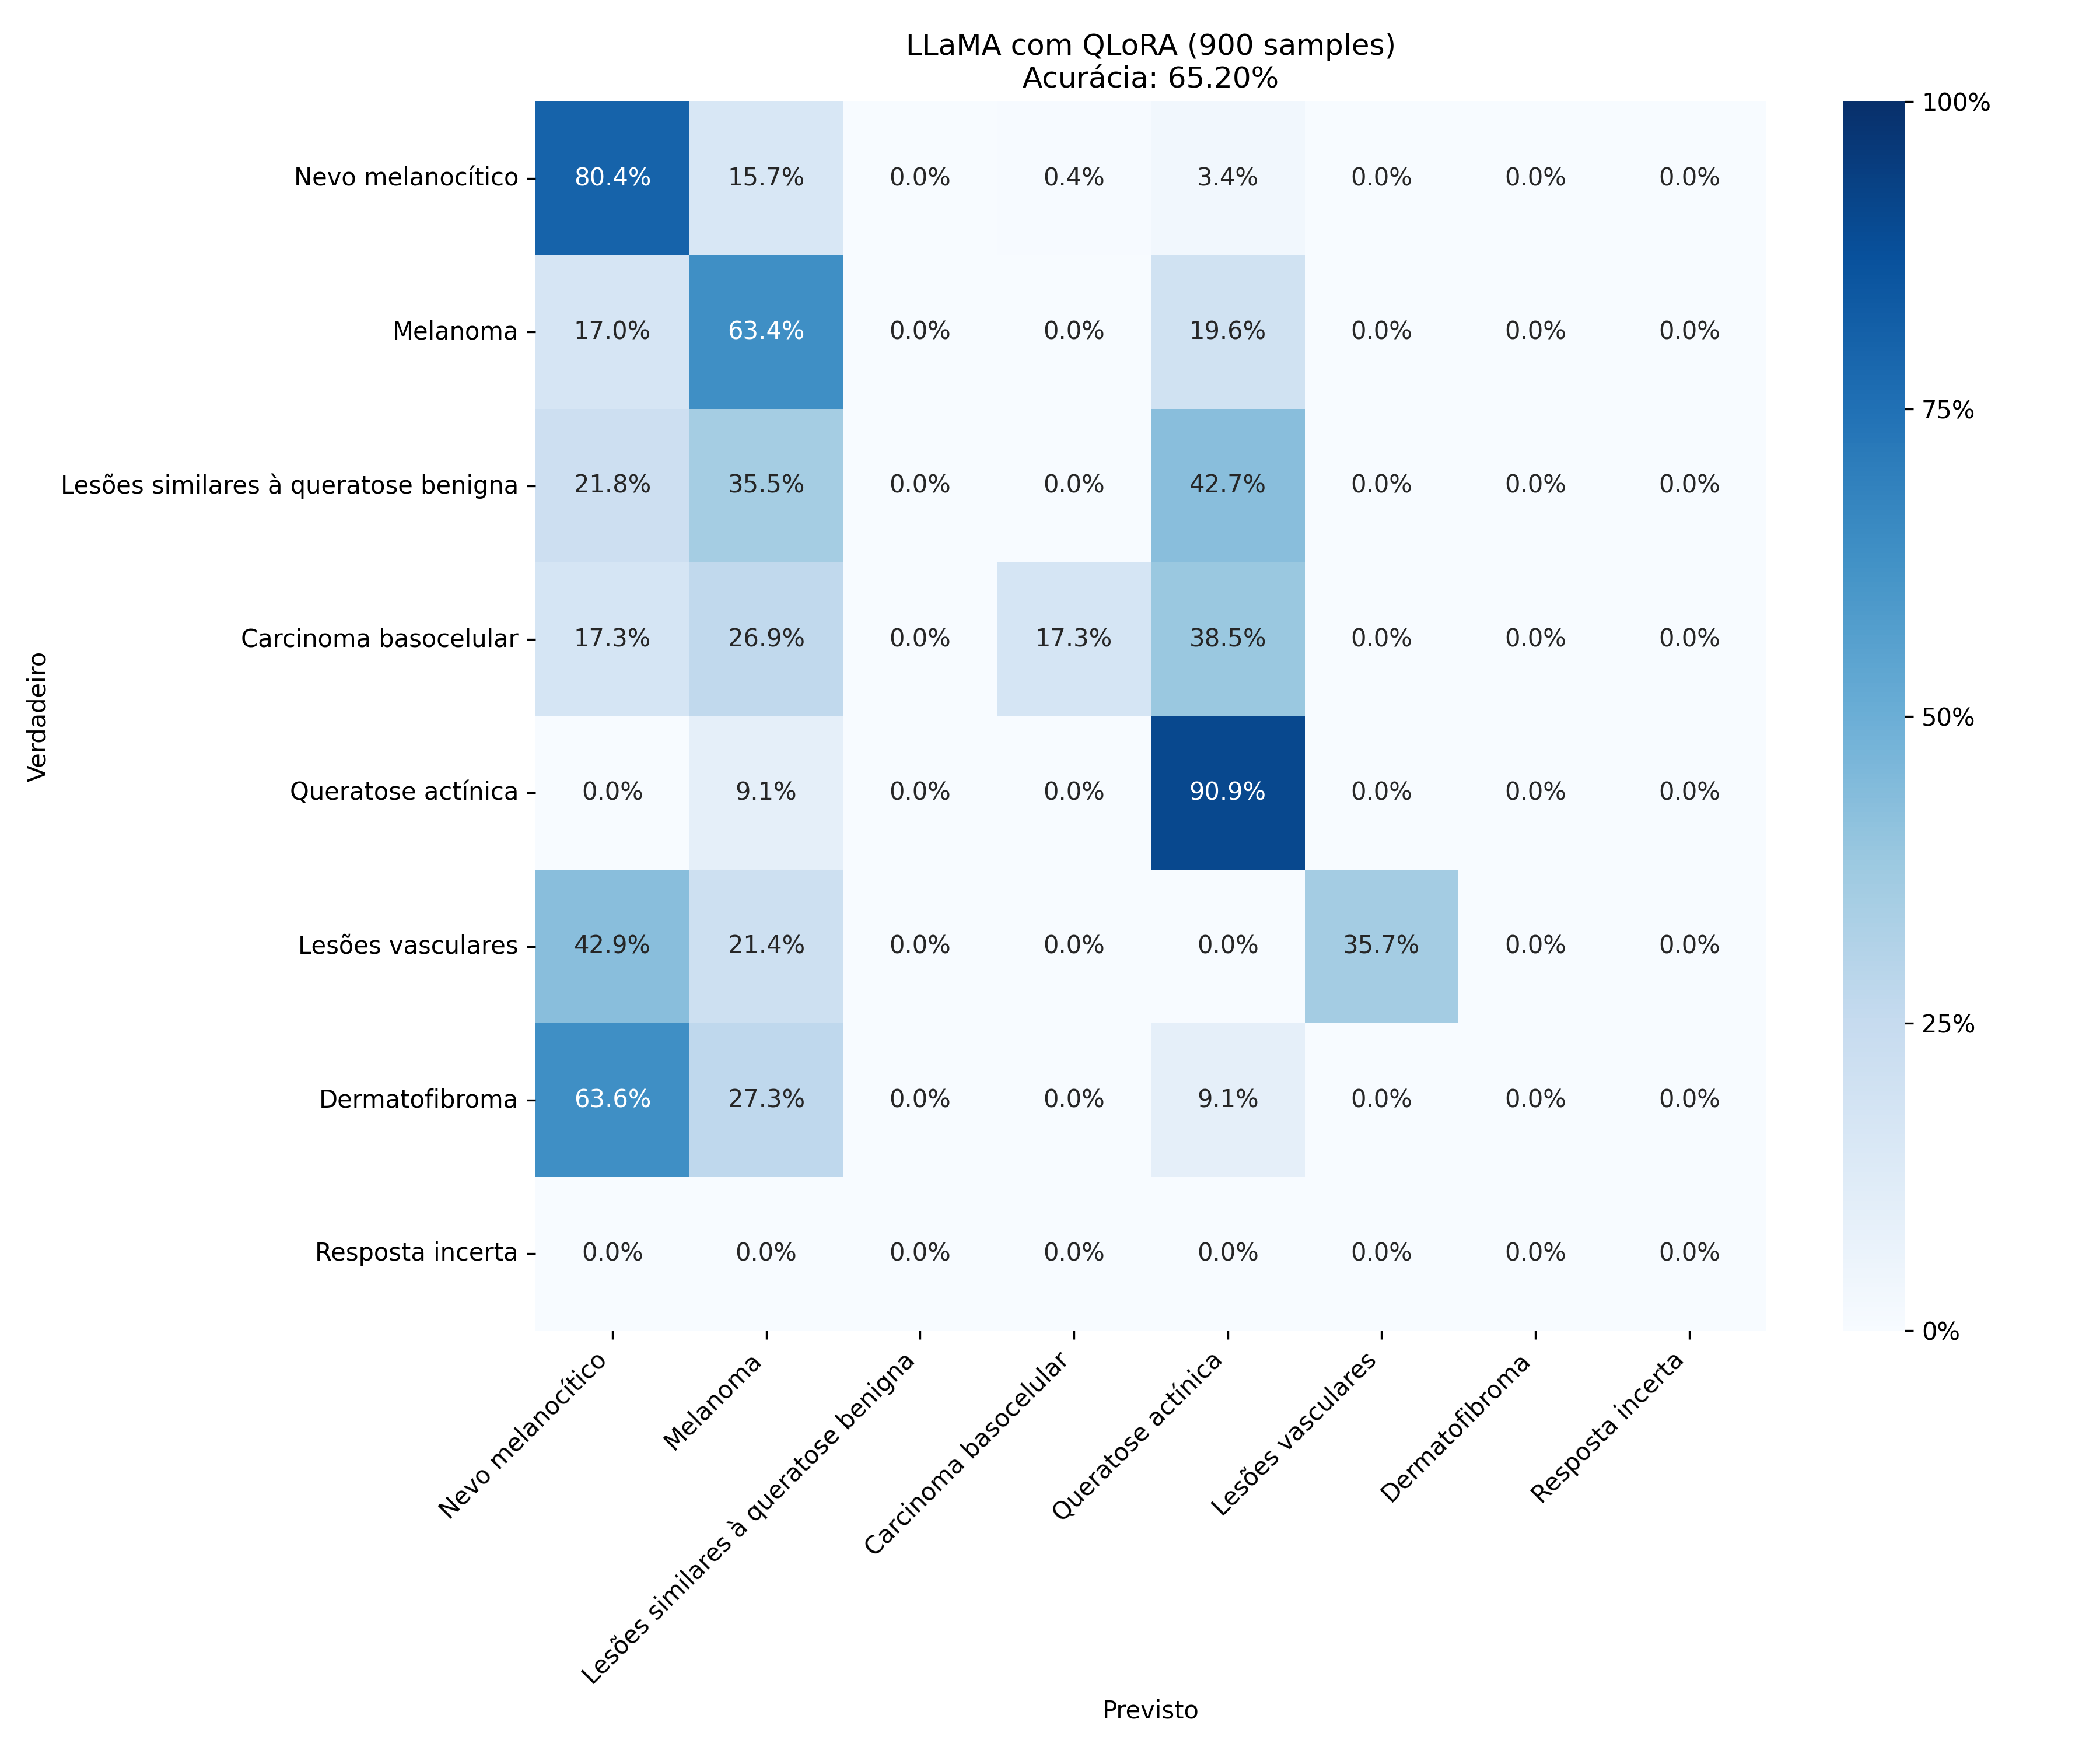
\includegraphics[width=1\columnwidth,keepaspectratio]{images/confusion_matrix_qlora_900.png}
    \label{fig:confusion_matrix_qlora_900}
    \fonte{Autoria própria.}
\end{figure}

\clearpage

\begin{figure}[ht]
    \centering
    \caption{\small Matriz de confusão para o \ac{LLaMA} treinado com \ac{LoRA} e 900 amostras.}
    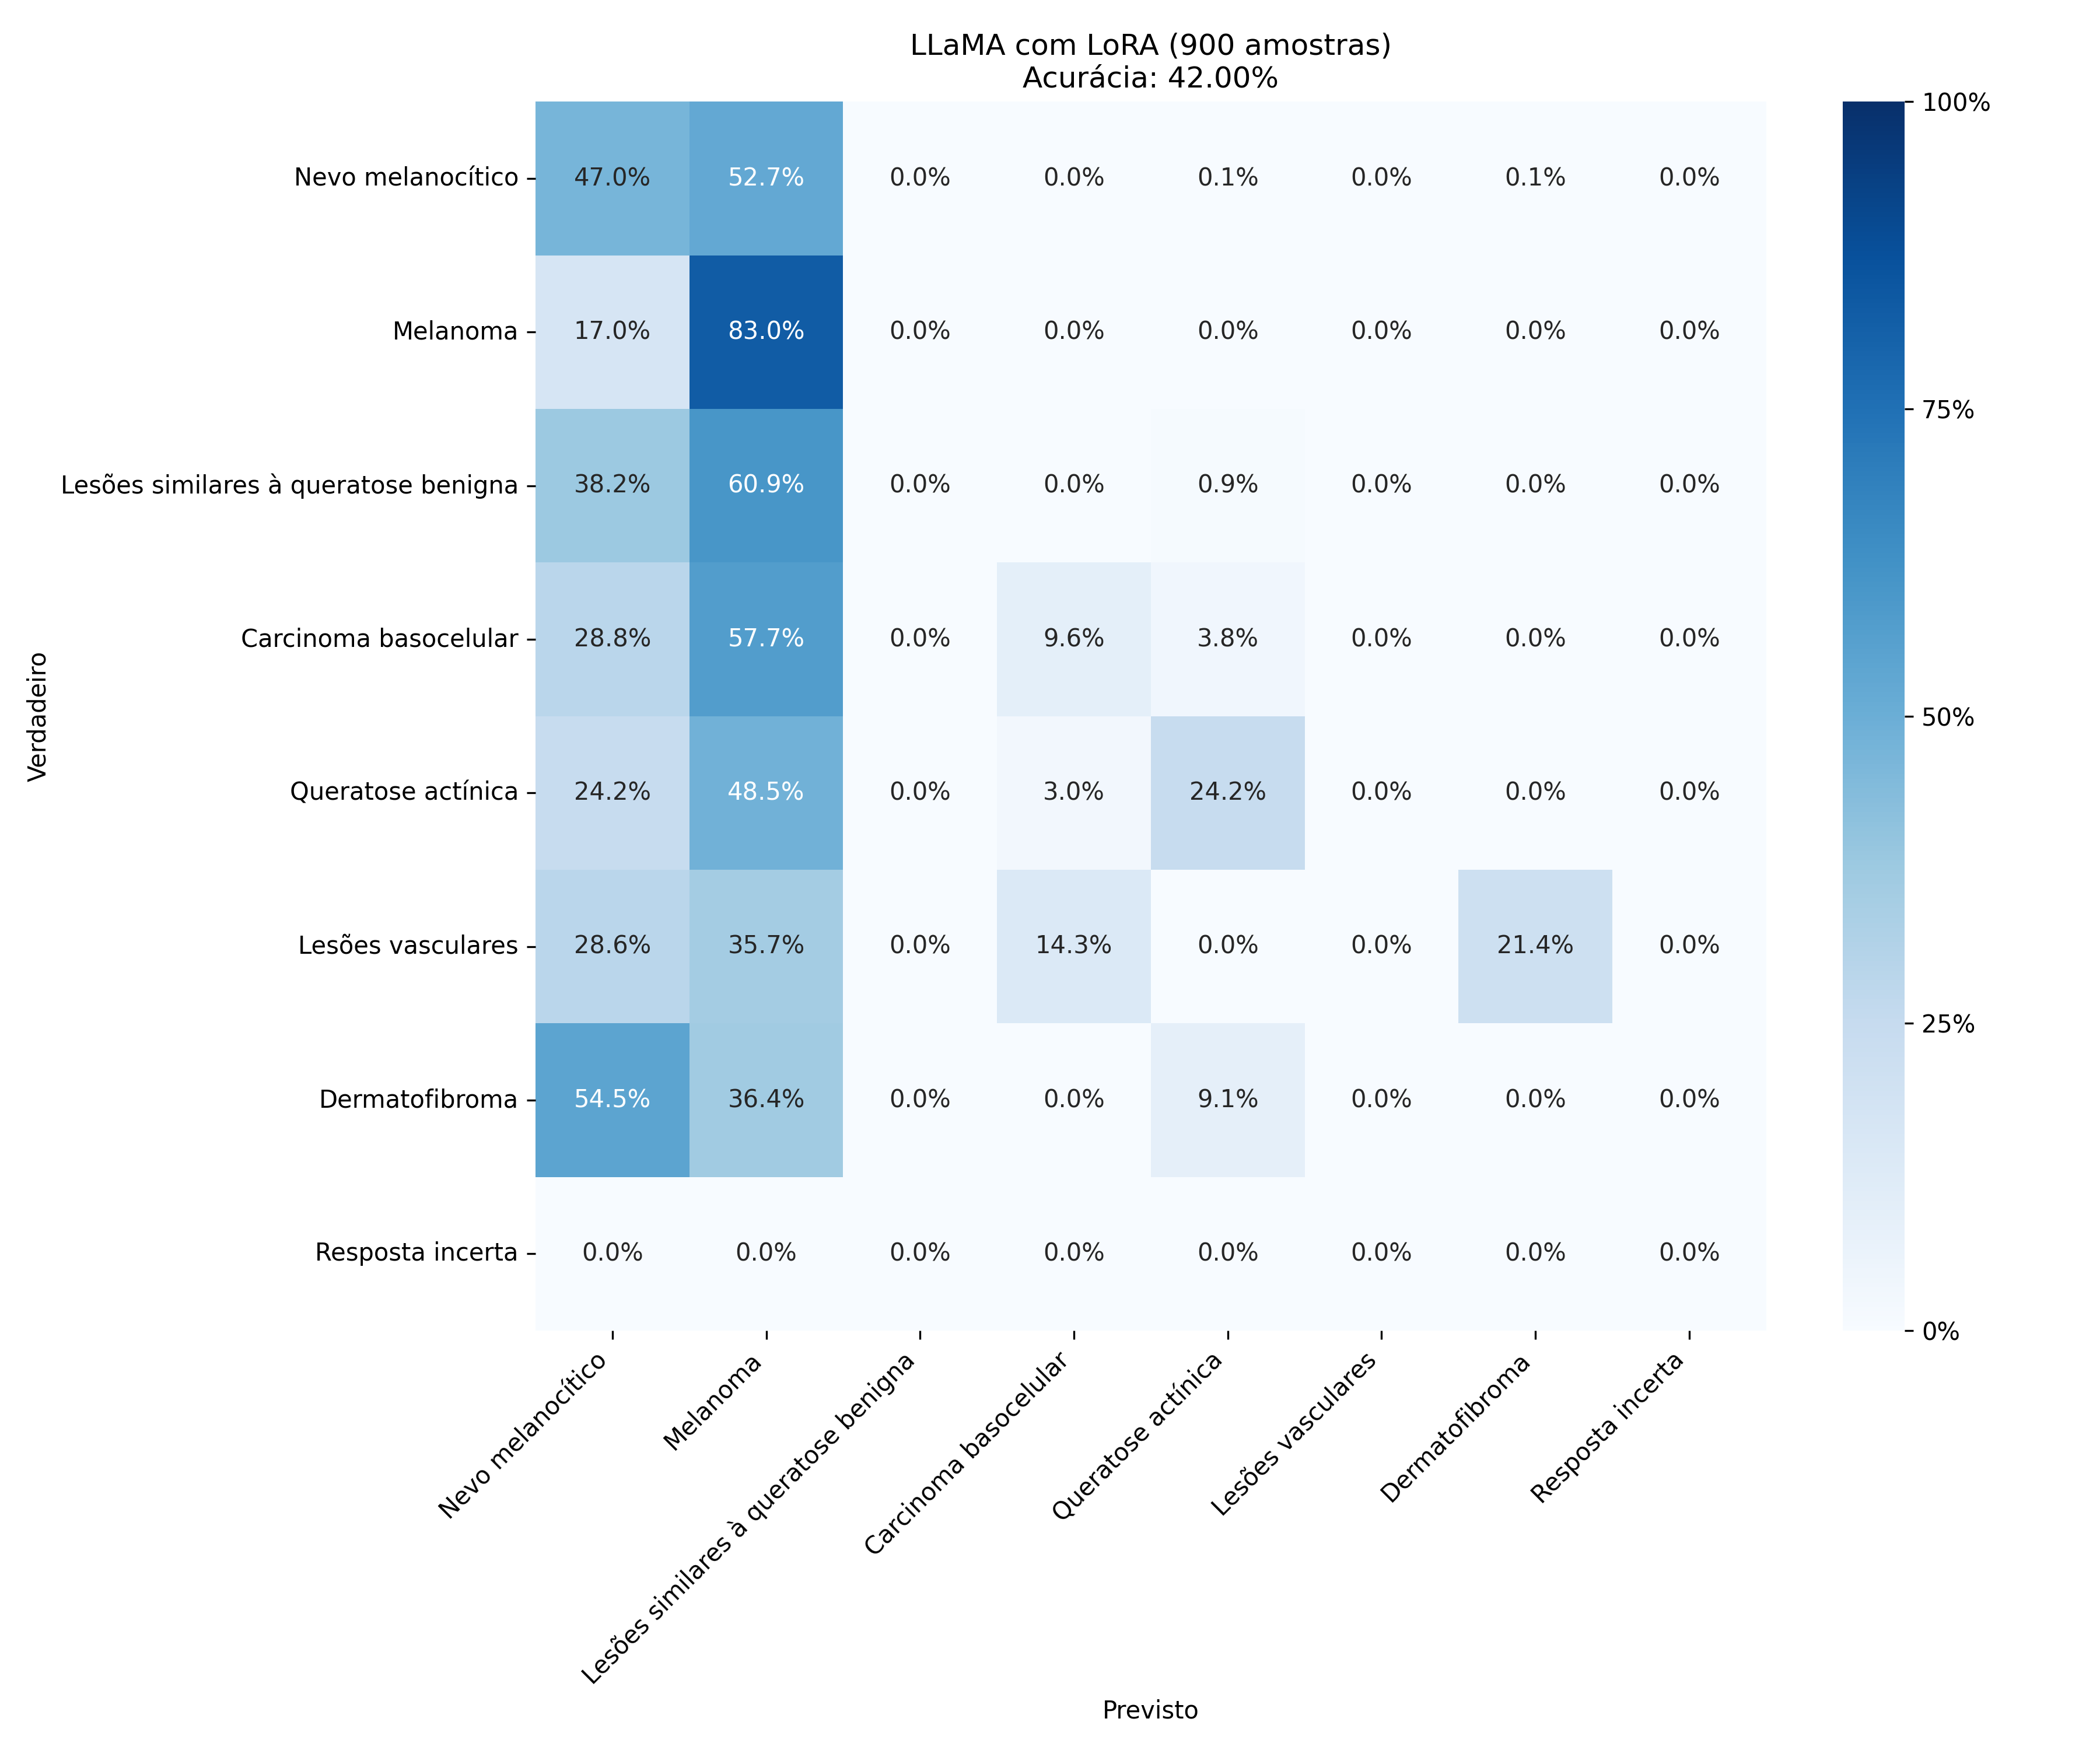
\includegraphics[width=1\columnwidth,keepaspectratio]{images/confusion_matrix_lora_900.png}
    \label{fig:confusion_matrix_lora_900}
    \fonte{Autoria própria.}
\end{figure}

O modelo treinado com \ac{QLoRA} e 1800 amostras teve um ganho de acurácia, atingindo 71,1\% e apresentando um padrão de reconhecimento melhor do que os modelos
anteriores. A matriz de confusão pode ser vista na \autoref{fig:confusion_matrix_qlora_1800}.

\clearpage

\begin{figure}[ht]
    \centering
    \caption{\small Matriz de confusão para o \ac{LLaMA} treinado com \ac{QLoRA} e 1800 amostras.}
    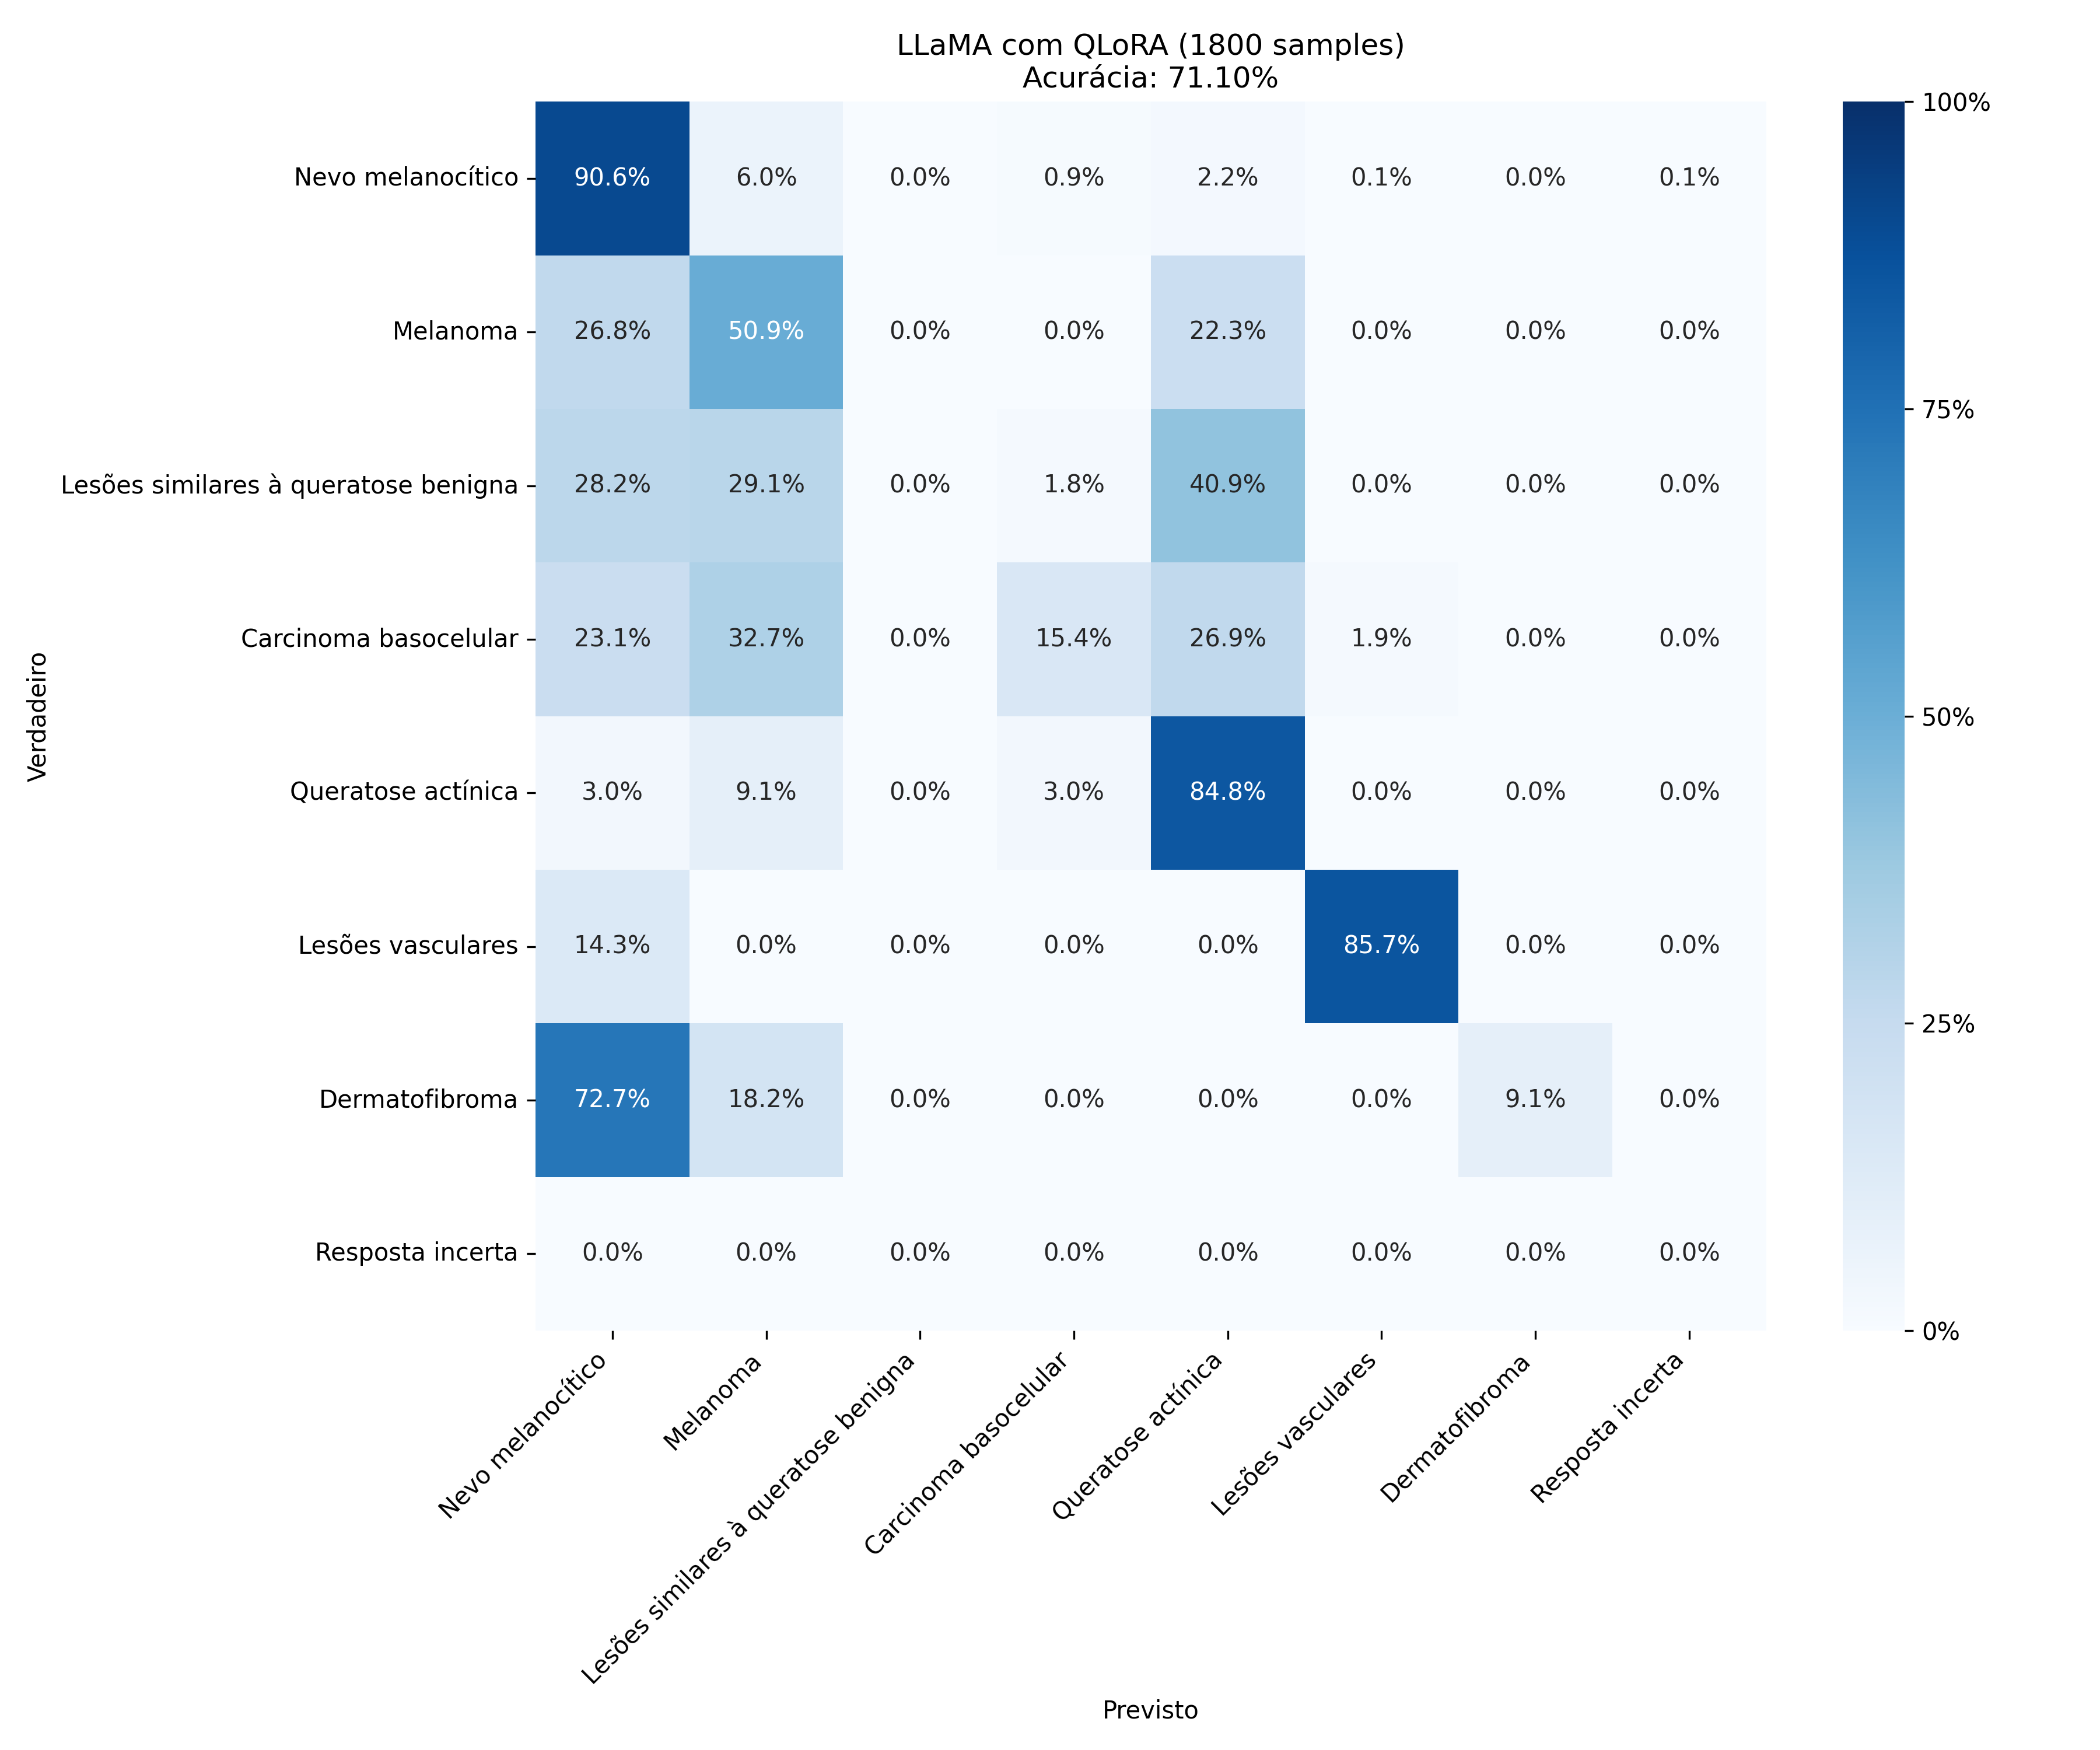
\includegraphics[width=1\columnwidth,keepaspectratio]{images/confusion_matrix_qlora_1800.png}
    \label{fig:confusion_matrix_qlora_1800}
    \fonte{Autoria própria.}
\end{figure}

Com 5000 amostras, ambos os modelos treinados com \ac{QLoRA} e \ac{LoRA} apresentaram resultados melhores, com 85,4\% e 86,2\% de acurácia, respectivamente. Deve-se
observar que as configurações de treinamento foram modificadas, sendo que os dois métodos utilizam hiperparâmetros similares. O \textit{fine-tuning} com \ac{LoRA} se
mostrou levemente melhor dessa vez, demonstrando que o baixo desempenho do \ac{LoRA} nos outros treinamentos foi por conta de uma escolha não ideal de hiperparâmetros.
A \autoref{fig:confusion_matrix_qlora_5000} e a \autoref{fig:confusion_matrix_lora_5000} apresentam esses resultados.

\clearpage

\begin{figure}[ht]
    \centering
    \caption{\small Matriz de confusão do \ac{LLaMA} treinado com \ac{QLoRA} e 5000 amostras.}
    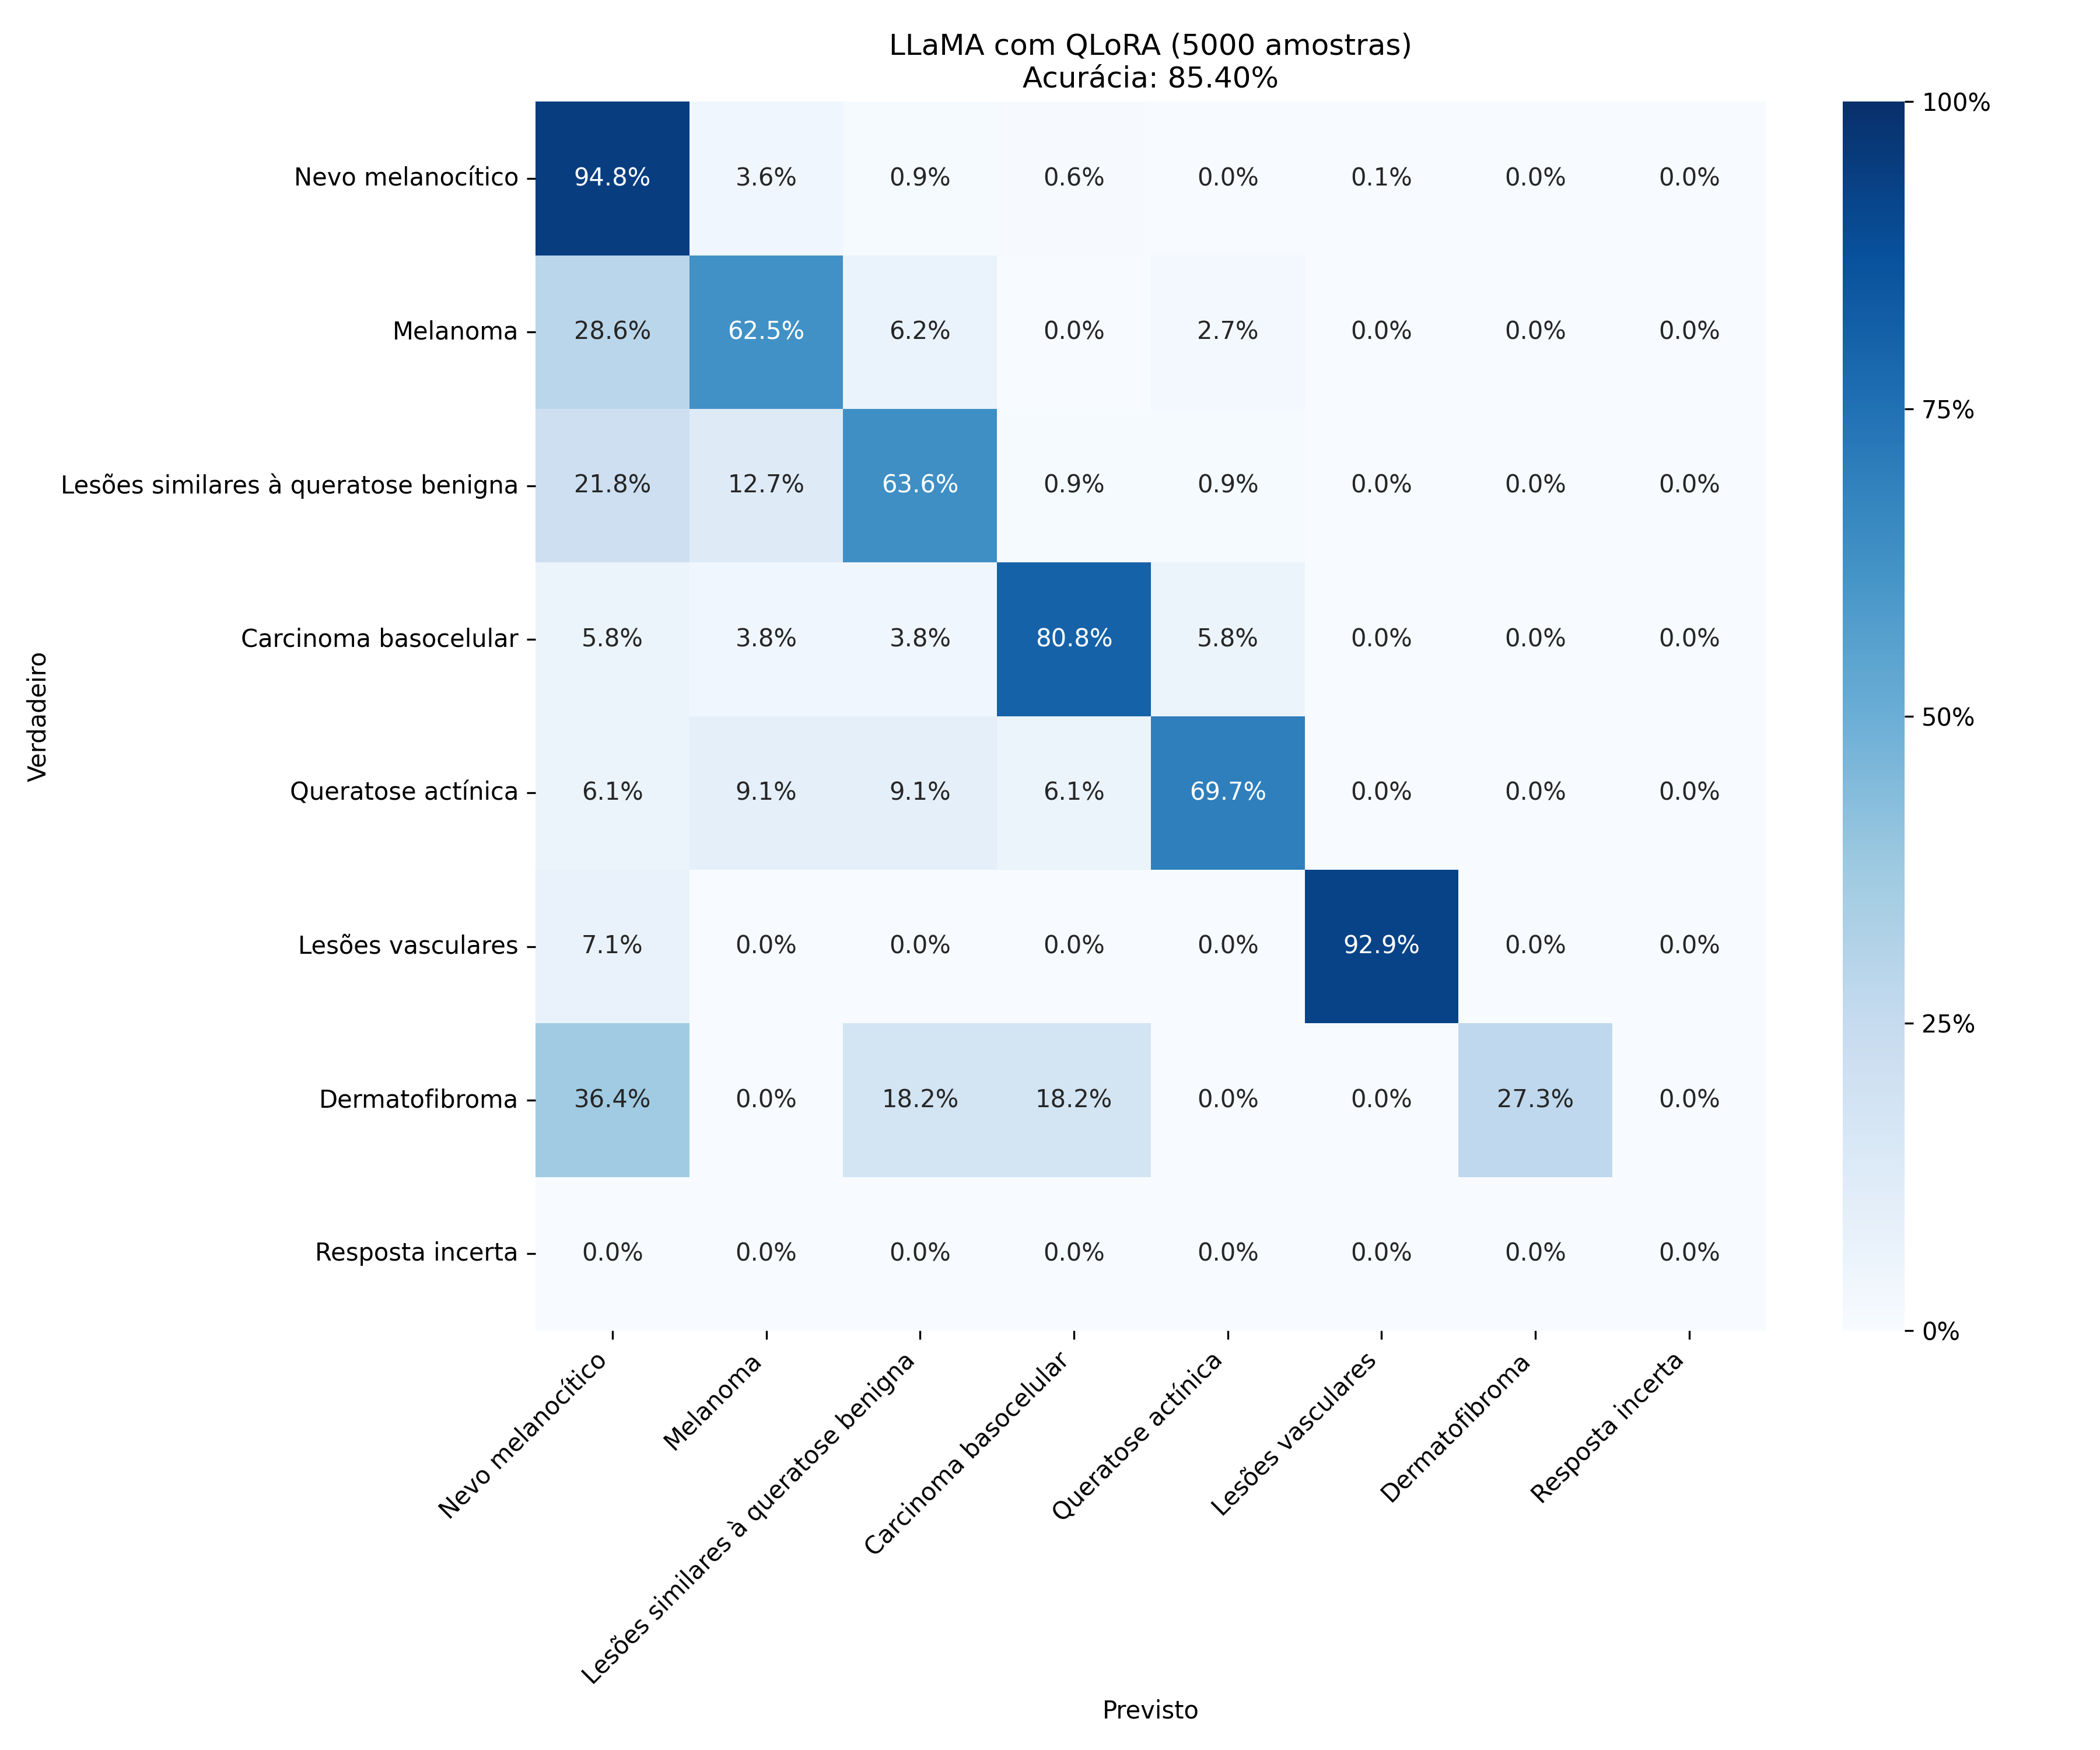
\includegraphics[width=1\columnwidth,keepaspectratio]{images/confusion_matrix_qlora_5000.png}
    \label{fig:confusion_matrix_qlora_5000}
    \fonte{Autoria própria.}
\end{figure}

\clearpage

\begin{figure}[ht]
    \centering
    \caption{\small Matriz de confusão para o \ac{LLaMA} treinado com \ac{LoRA} e 5000 amostras.}
    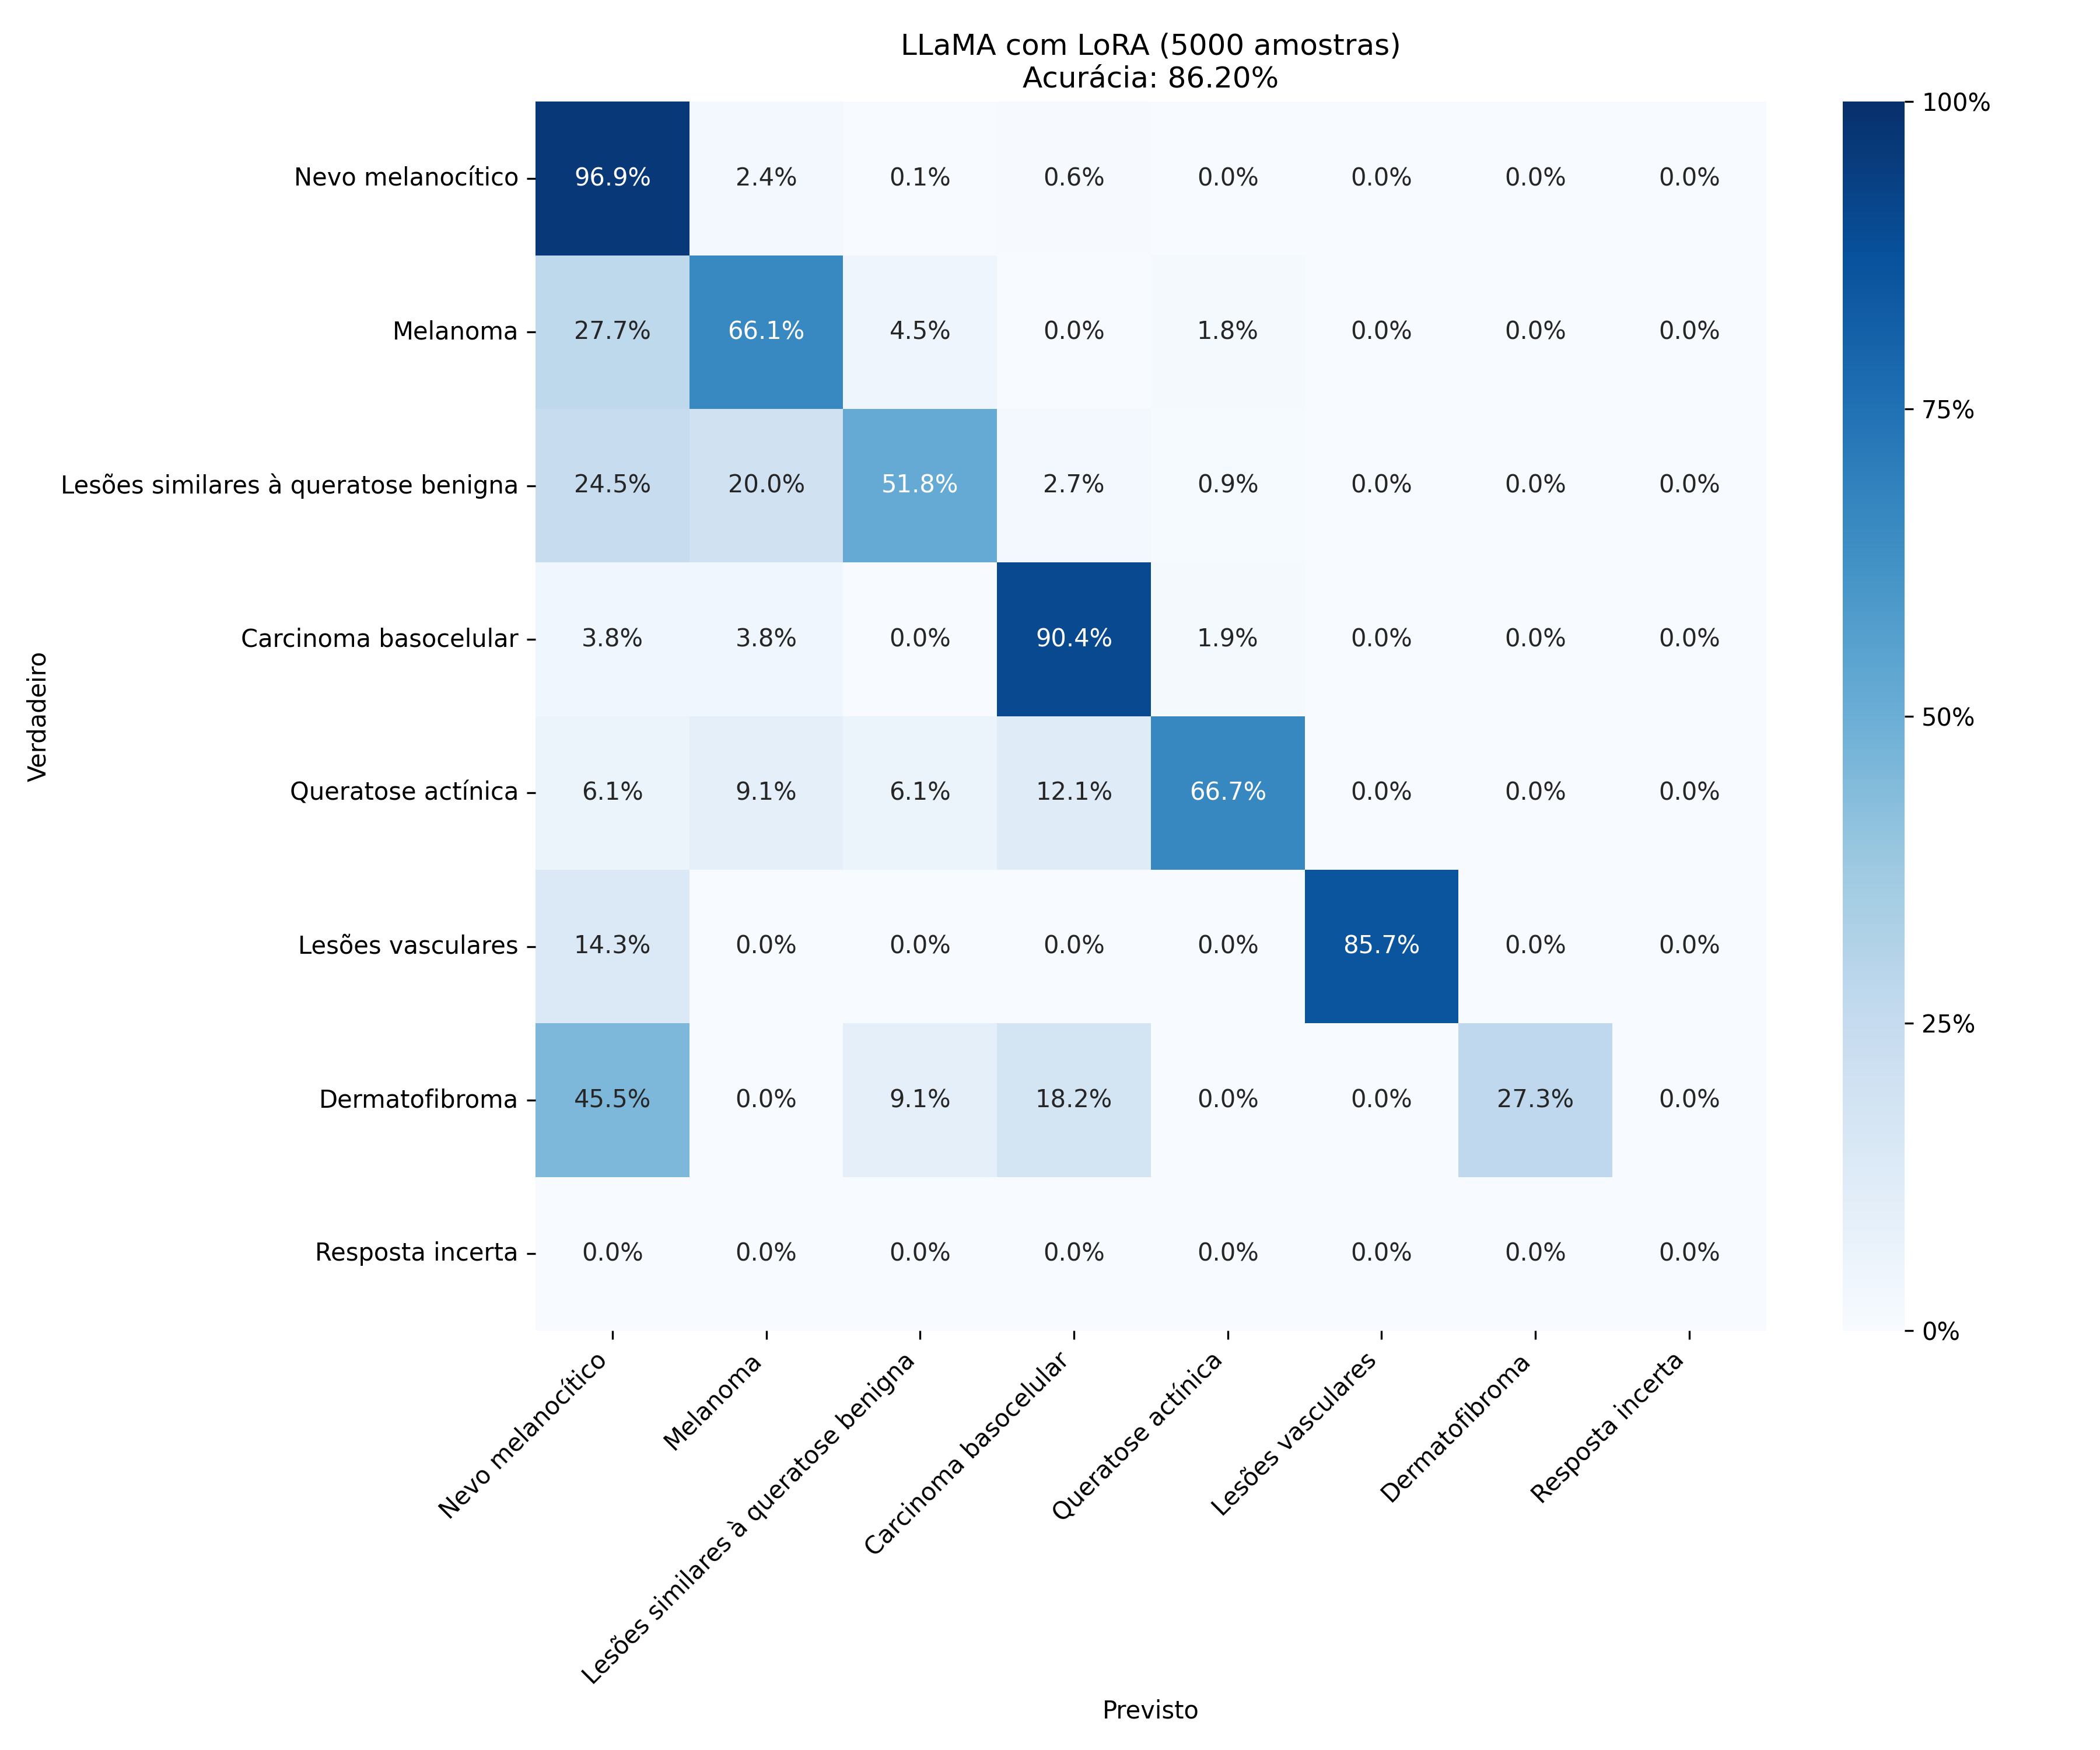
\includegraphics[width=1\columnwidth,keepaspectratio]{images/confusion_matrix_lora_5000.png}
    \label{fig:confusion_matrix_lora_5000}
    \fonte{Autoria própria.}
\end{figure}

Por último, o \ac{LLaMA} treinado com \ac{QLoRA} e 9500 amostras apresentou os melhores resultados, com uma acurácia de 87,4\%. A matriz de confusão pode ser vista na
\autoref{fig:confusion_matrix_qlora_9500}.

A \autoref{tab:training_accuracies} apresenta as acurácias de forma resumida.

\begin{figure}[ht]
    \centering
    \caption{\small Matriz de confusão para o \ac{LLaMA} treinado com \ac{QLoRA} e 9500 amostras.}
    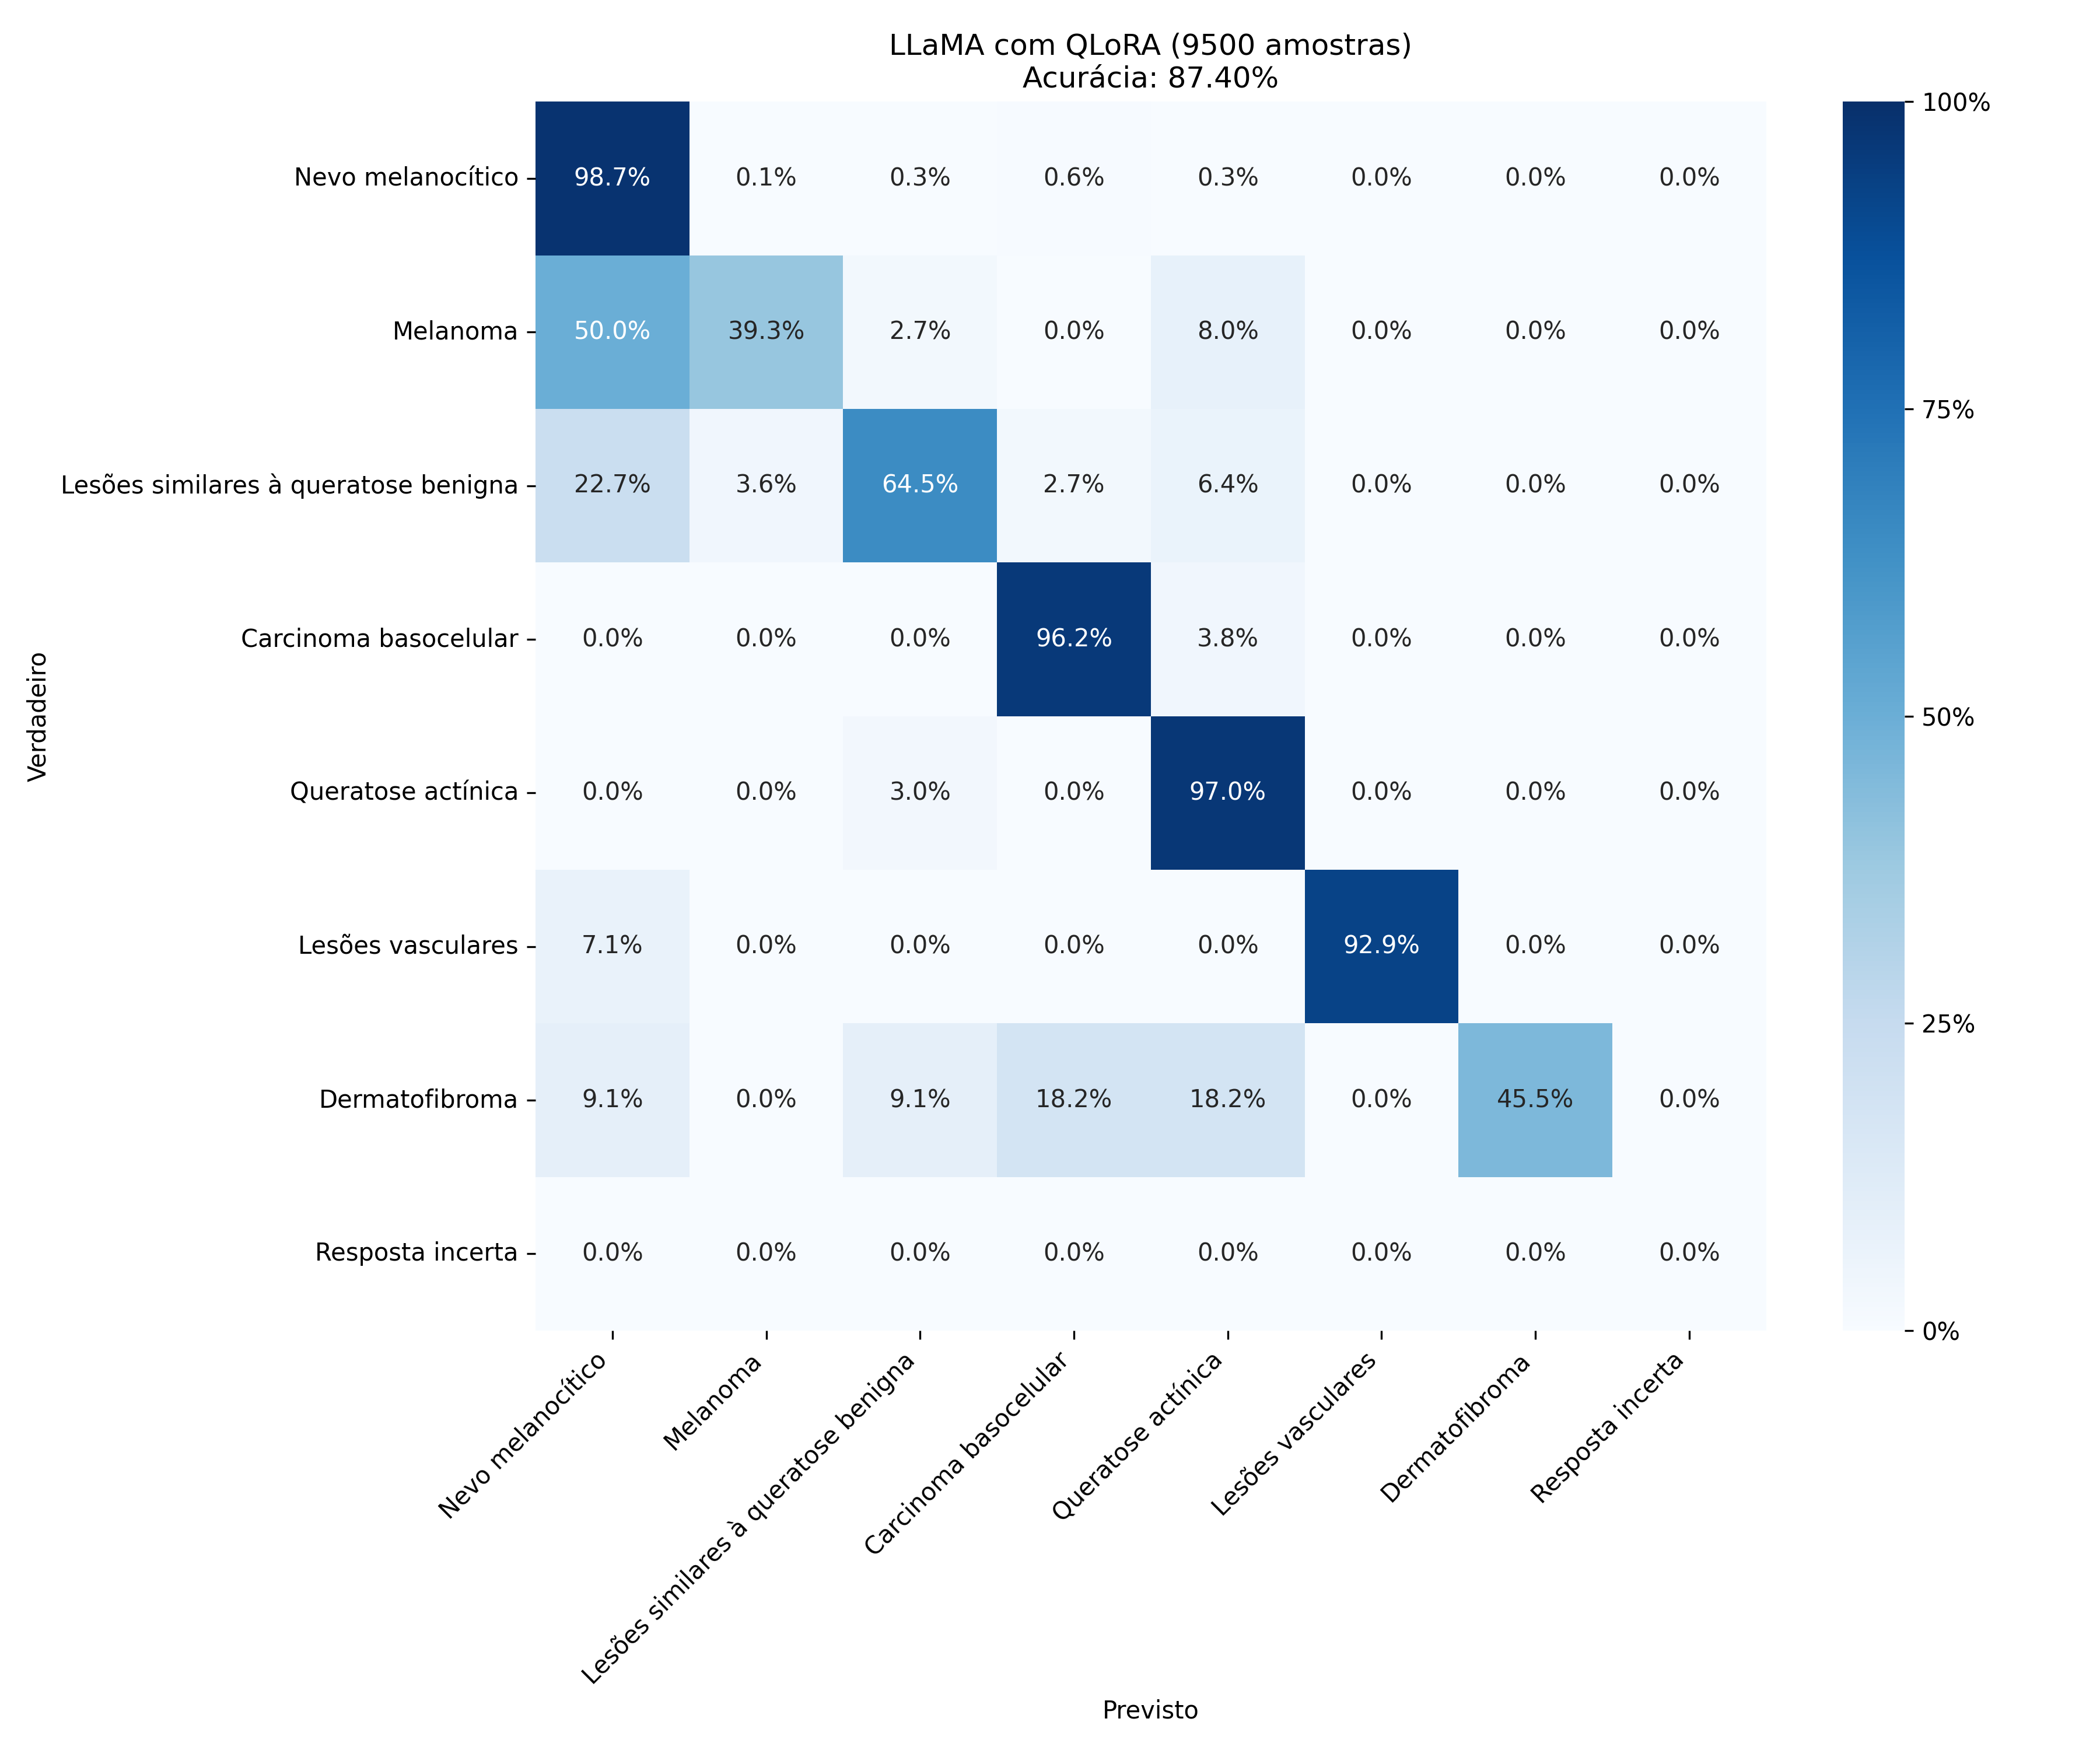
\includegraphics[width=1\columnwidth,keepaspectratio]{images/confusion_matrix_qlora_9500.png}
    \label{fig:confusion_matrix_qlora_9500}
    \fonte{Autoria própria.}
\end{figure}

\begin{table}[ht]
    \caption{\small Acurácia de cada modelo treinado.}
    \centering
    \begin{tabular}{l|c|c}
        \hline
        Método                      & Quantidade de amostras & Acurácia (\%) \\ \hline
        \multirow{5}{*}{\ac{QLoRA}} & 450                    & 65,5          \\
                                    & 900                    & 65,2          \\
                                    & 1800                   & 71,1          \\
                                    & 5000                   & 85,4          \\
                                    & 9500                   & 87,4          \\ \hline
        \multirow{3}{*}{\ac{LoRA}}  & 450                    & 49,5          \\
                                    & 900                    & 42,0          \\
                                    & 5000                   & 86,2          \\ \hline
    \end{tabular}
    \label{tab:training_accuracies}
    \fonte{Autoria própria}
\end{table}
